\chapter{有限元无网格混合离散方案}

本章针对体积不可压问题建立有限元无网格混合离散分析方法,调整体积约束比以达到最优约束比。
首先介绍了再生核近似无网格法,详细说明了无网格形函数的构造过程.
其次,结合对LBB稳定系数的分析,提出满足LBB稳定性条件的免体积自锁混合离散方案。
最后,通过典型弹性力学算例验证所提混合离散方案的稳定性与正确性。
\section{再生核近似}
为达到最优体积约束比,采用如图\ref{ch_4:fig:meshfree}所示的有限元无网格混合离散方案离散位移和压力节点。
将伽辽金弱形式\eqref{ch_2:eq:weak_mix}中的位移$\boldsymbol{u}$和压力$p$采用不同的离散方式进行近似。
位移$\boldsymbol{u}$仍采用有限元形函数\eqref{ch_2:eq:u_h_mix}进行近似,而压力$p$通过再生核无网格形函数进行近似。
再生核无网格近似将求解域$\Omega$及其边界$\Gamma$由$n_p$个无网格节点离散$\{\boldsymbol x_K\}_{K=1}^{n_p}$。每个无网格节点$\boldsymbol x_K$对应的形函数为$\Psi_K(\boldsymbol{x})$,形函数影响域为$supp(\boldsymbol{x}_K)$。近似的压力$p_h$可表示为:
\begin{equation}
    p_h(\boldsymbol x) = \sum_{K=1}^{n_p} \Psi_K(\boldsymbol x) p_K
\end{equation}
其中$p_K$为与无网格节点$x_K$对应的节点系数。
\begin{figure}[H]
    \centering 
        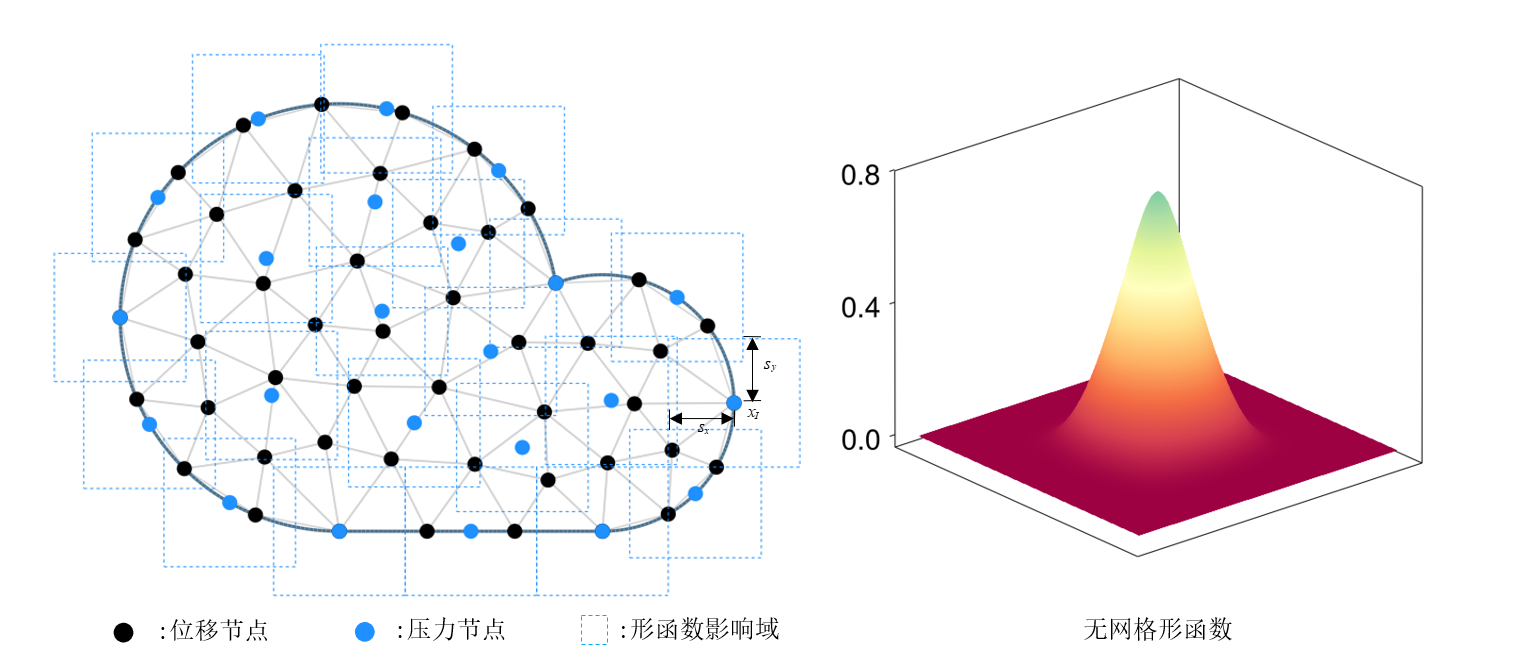
\includegraphics[scale=0.5]{figures/meshfree.png}
        \caption{有限元无网格混合离散示意图}\label{ch_4:fig:meshfree}
\end{figure}

根据再生核近似理论\cite{liu1995},无网格形函数可以假设为如下形式:
\begin{equation}\label{ch_4:eq:rkshape}
    \Psi_K(\boldsymbol x) = \boldsymbol c(\boldsymbol x_K-\boldsymbol x) \boldsymbol p^{[n]}(\boldsymbol x_K-\boldsymbol x) \phi(\boldsymbol x_K - \boldsymbol x)
\end{equation}
其中$\boldsymbol p$为$n$阶基函数向量,其表达式为:
\begin{equation}
    \boldsymbol p^{[n]}(\boldsymbol x) = \{ 1, x, y, x^2, xy, y^2,...,y^n\}^\mathrm{T}
\end{equation}
对于弹性力学问题,无网格基函数一般选择二阶或者三阶多项式基函数,本文选择二阶多项式基函数:
\begin{equation}
    \boldsymbol p(\boldsymbol x) = \{ 1, x, y, x^2, xy, y^2\}^\mathrm{T}
\end{equation}
而$\phi$为核函数,其影响域的大小由影响域尺寸$s$决定,核函数及其影响域的大小共同决定了无网格形函数的局部紧支性和光滑性。在二维情况下,核函数的影响域通常为圆形或者矩形。本文的影响域形状为矩形,矩形影响域的核函数可由下列公式计算得到:
\begin{equation}
    \phi(\boldsymbol x_K-\boldsymbol x) = \phi(r_x) \phi(r_y), \quad r_x = \frac{|x_K - x|}{s_{x}},r_y = \frac{| y_K -  y|}{s_{y}}
\end{equation}
其中, $s_x$ 和 $s_y$ 分别为 $x$ 和 $y$ 方向上的影响域尺寸,若节点均匀布置,一般使两个方向上的影响域大小相等,即$s_x = s_y = s$。
为保证形函数的紧支性和光滑性,$\phi$ 通常取为阶次大于 $n$ 的紧支函数。因此,本文核函数 $\phi(\boldsymbol x_K-\boldsymbol x)$ 取为三次样条函数:
\begin{equation}
    \phi(s) =\frac{1}{3!} \begin{cases}
        (2-2s)^3 - 4(1-2s)^3 & s\le\frac{1}{2} \\
        (2-2s)^3 &\frac{1}{2}<s<1 \\
        0 & s> 1
    \end{cases}
\end{equation}
$\boldsymbol c$为待定系数向量,可以通过满足下列一致性条件确定:
\begin{equation}\label{ch_4:eq:cc1}
    \sum_{I=1}^{n_p}\Psi_K(\boldsymbol x) \boldsymbol p(\boldsymbol x_K) = \boldsymbol p (\boldsymbol x)
\end{equation}
或等效的转换形式:
\begin{equation}\label{ch_4:eq:cc2}
    \sum_{I=1}^{n_p}\Psi_K(\boldsymbol x) \boldsymbol p(\boldsymbol x_K-\boldsymbol x) = \boldsymbol p(\boldsymbol 0)
\end{equation}
将式\eqref{ch_4:eq:rkshape}代入式\eqref{ch_4:eq:cc2}中即可得到待定系数向量$\boldsymbol c$的具体表达式:
\begin{equation}\label{ch_4:eq:correction}
    \boldsymbol c(\boldsymbol x_K-\boldsymbol x) = \boldsymbol A^{-1}(\boldsymbol x_K-\boldsymbol x)\boldsymbol p(\boldsymbol 0)
\end{equation}
式中$\boldsymbol A$为矩量矩阵:
\begin{equation}
    \boldsymbol A(\boldsymbol x_K-\boldsymbol x) = \sum_{I=1}^{n_p}\boldsymbol p(\boldsymbol x_K-\boldsymbol x) \boldsymbol p^{\mathrm{T}}(\boldsymbol x_K-\boldsymbol x)\phi(\boldsymbol x_K-\boldsymbol x)
\end{equation}

将式\eqref{ch_4:eq:correction}代入式\eqref{ch_4:eq:rkshape}可得最终的再生核无网格形函数表达式:
\begin{equation}\label{ch_4:eq:mfshapefunction}
    \Psi_K(\boldsymbol x) = \boldsymbol p^{\mathrm{T}}(\boldsymbol 0) \boldsymbol A^{-1}(\boldsymbol x_K-\boldsymbol x)p(\boldsymbol x_K-\boldsymbol x)\phi(\boldsymbol x_K-\boldsymbol x)
\end{equation}

\section{满足LBB稳定性条件的混合离散方案}
基于考虑约束比的LBB稳定系数估计式\eqref{ch_3:eq:r3}和最优体积约束比取值范围\eqref{ch_3:eq:best},结合有限元无网格混合离散分析方法,对有限元离散单元在不同约束比例下的LBB稳定系数进行了系统性测试。
为探究单元类型和网格密度对计算结果的影响,测试选取了四种典型有限元离散单元:Tri3(三角形3节点单元)、Tri6(三角形6节点单元)、Quad4(四边形4节点单元)、Quad8(四边形八节点单元)和四个不同数量的位移节点($n_u=$25、81、289、1089)进行对比分析,旨在寻找出最优的免体积自锁有限元无网格混合离散方案。
所得测试结果如图\ref{ch_4:fig:infsup_convergence}所示。

以Tri3单元为例,图\eqref{ch_3:eq:best}(a)中的红色曲线反映了在位移节点数$n_u$固定的情况下,压力节点数$n_p$的变化对LBB稳定系数$\beta$的影响。
$\beta$值越接近于1表示该约束比例下的混合方案稳定性越好,(即满足LBB稳定性条件)。
图中四个竖向虚线分别表示四个不同位移节点数$n_u$对应的最优体积约束比下压力节点数$n_p$。
测试结果表明:当压力节点数$n_p$小于最优值(位于虚线左侧)时,离散方案趋于稳定,满足LBB稳定性条件;
而当$n_p$大于最优值(位于虚线右侧)时,离散方案则表现出不稳定性,无法满足LBB稳定性条件。
值得注意的是,传统有限元混合离散方案中采用的最优约束比($r=2$)对应的$\beta$值均位于虚线右侧,这表明传统有限元混合离散方案不满足LBB稳定性条件。

如图\ref{ch_4:fig:infsup_convergence}(b)、(c)、(d)所示,Tri6单元、Quad4单元和Quad8单元的测试结果与Tri3单元的基本一致。为保证混合离散方案在满足LBB稳定性条件的同时,避免使用两套网格进行离散而增加计算量,本研究基于上述测试结果,提出了如图\ref{ch_4:fig:mix_scheme}所示的免体积自锁有限元无网格混合离散方案。该方案的压力节点选取直接基于位移节点,从而实现了方案的简易性与稳定性。
图\ref{ch_4:fig:infsup_convergence}中实线折现展示了相应方案下的$\beta$取值,初步验证了该方案的可行性。

\begin{figure}[H]
    \centering
    \begin{subcaptiongroup}
    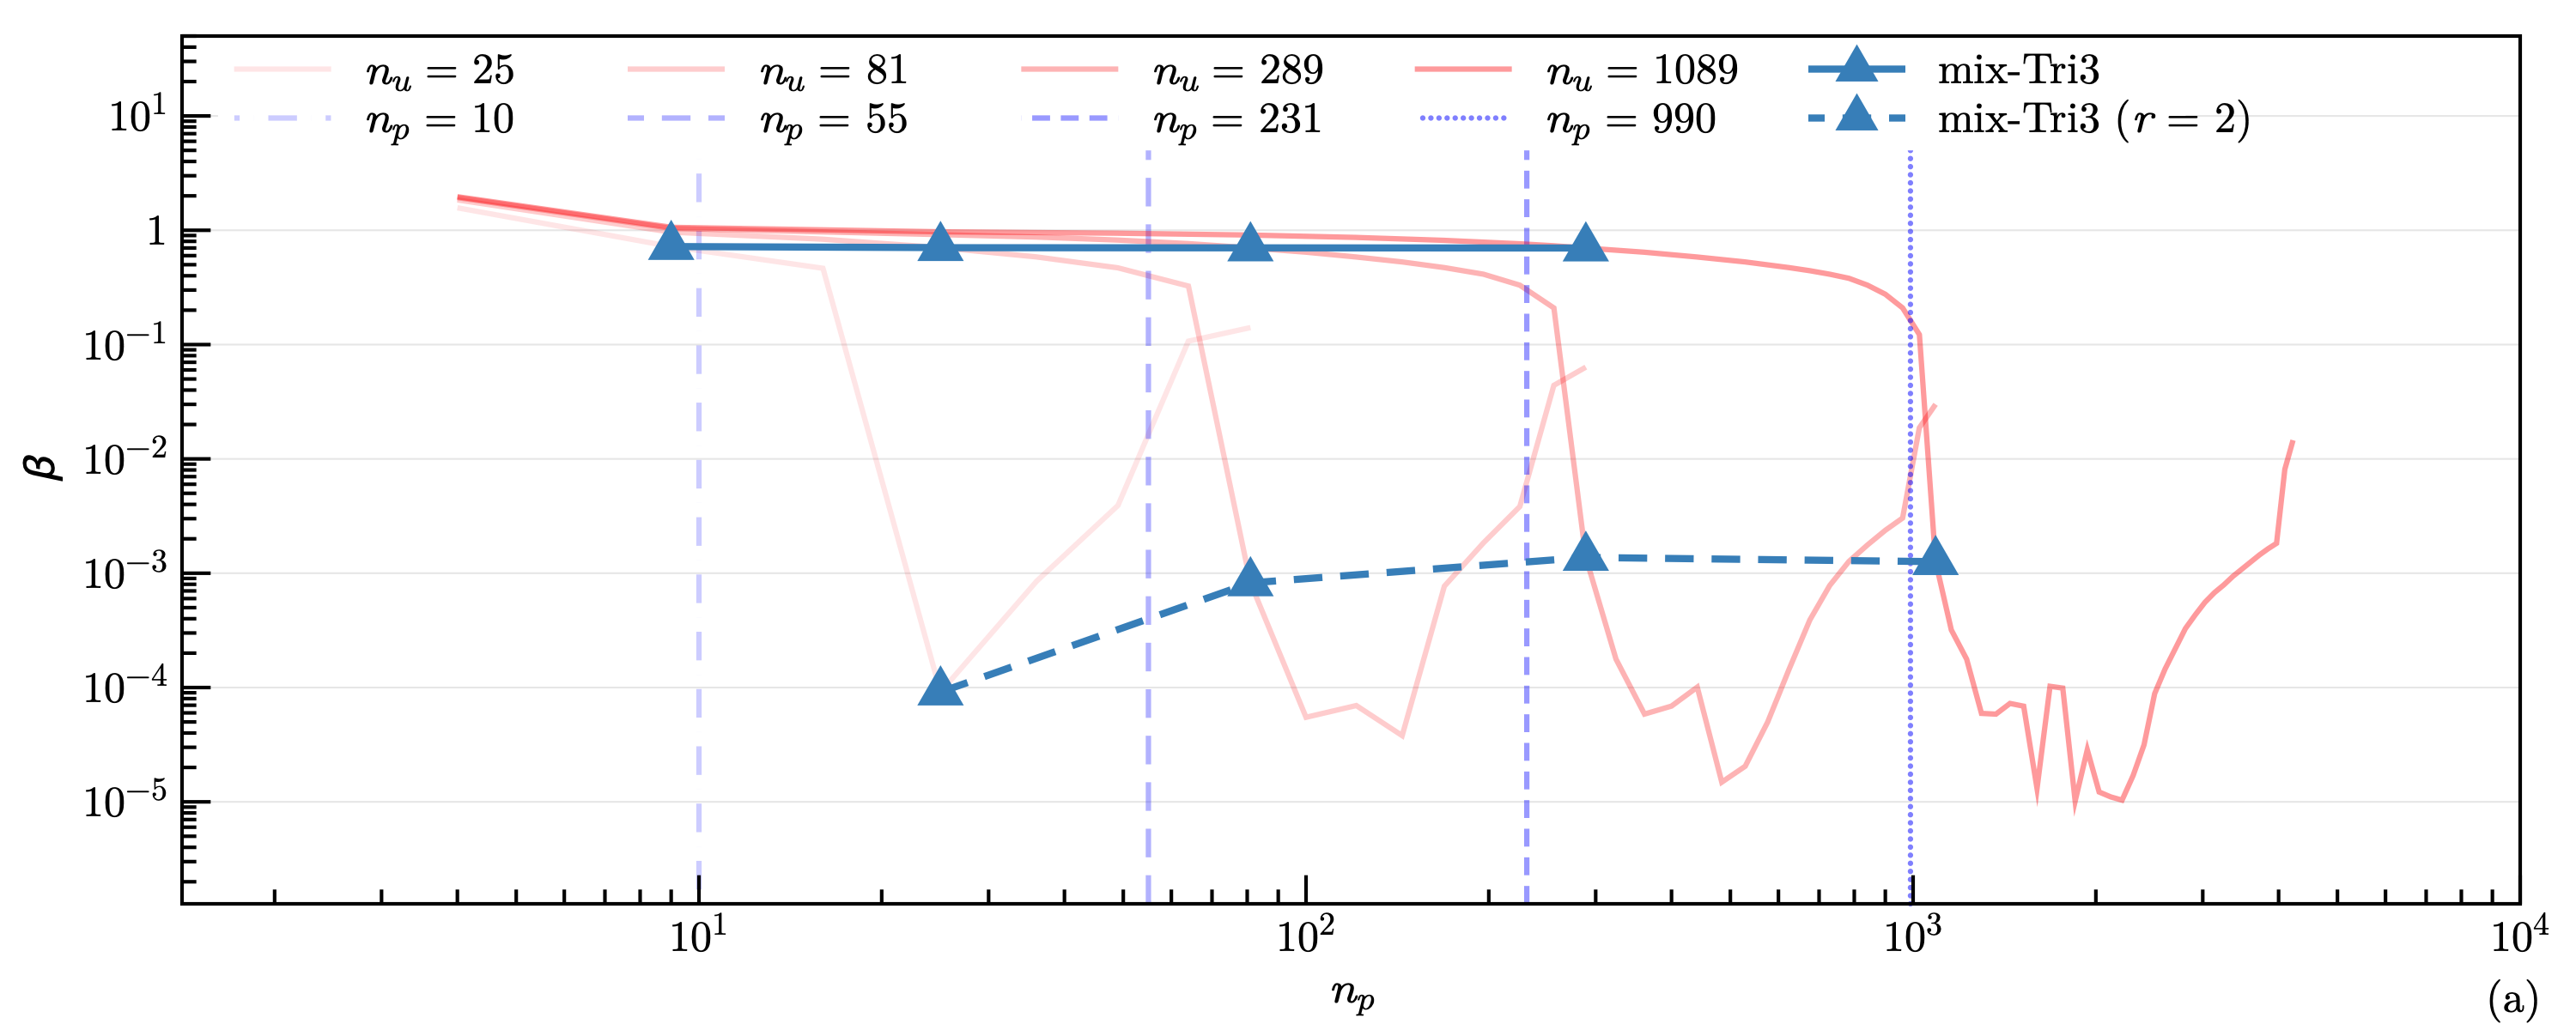
\includegraphics[width=0.9\textwidth]{figures/ch_4/infsup_tri3.png}\phantomcaption\label{a}
    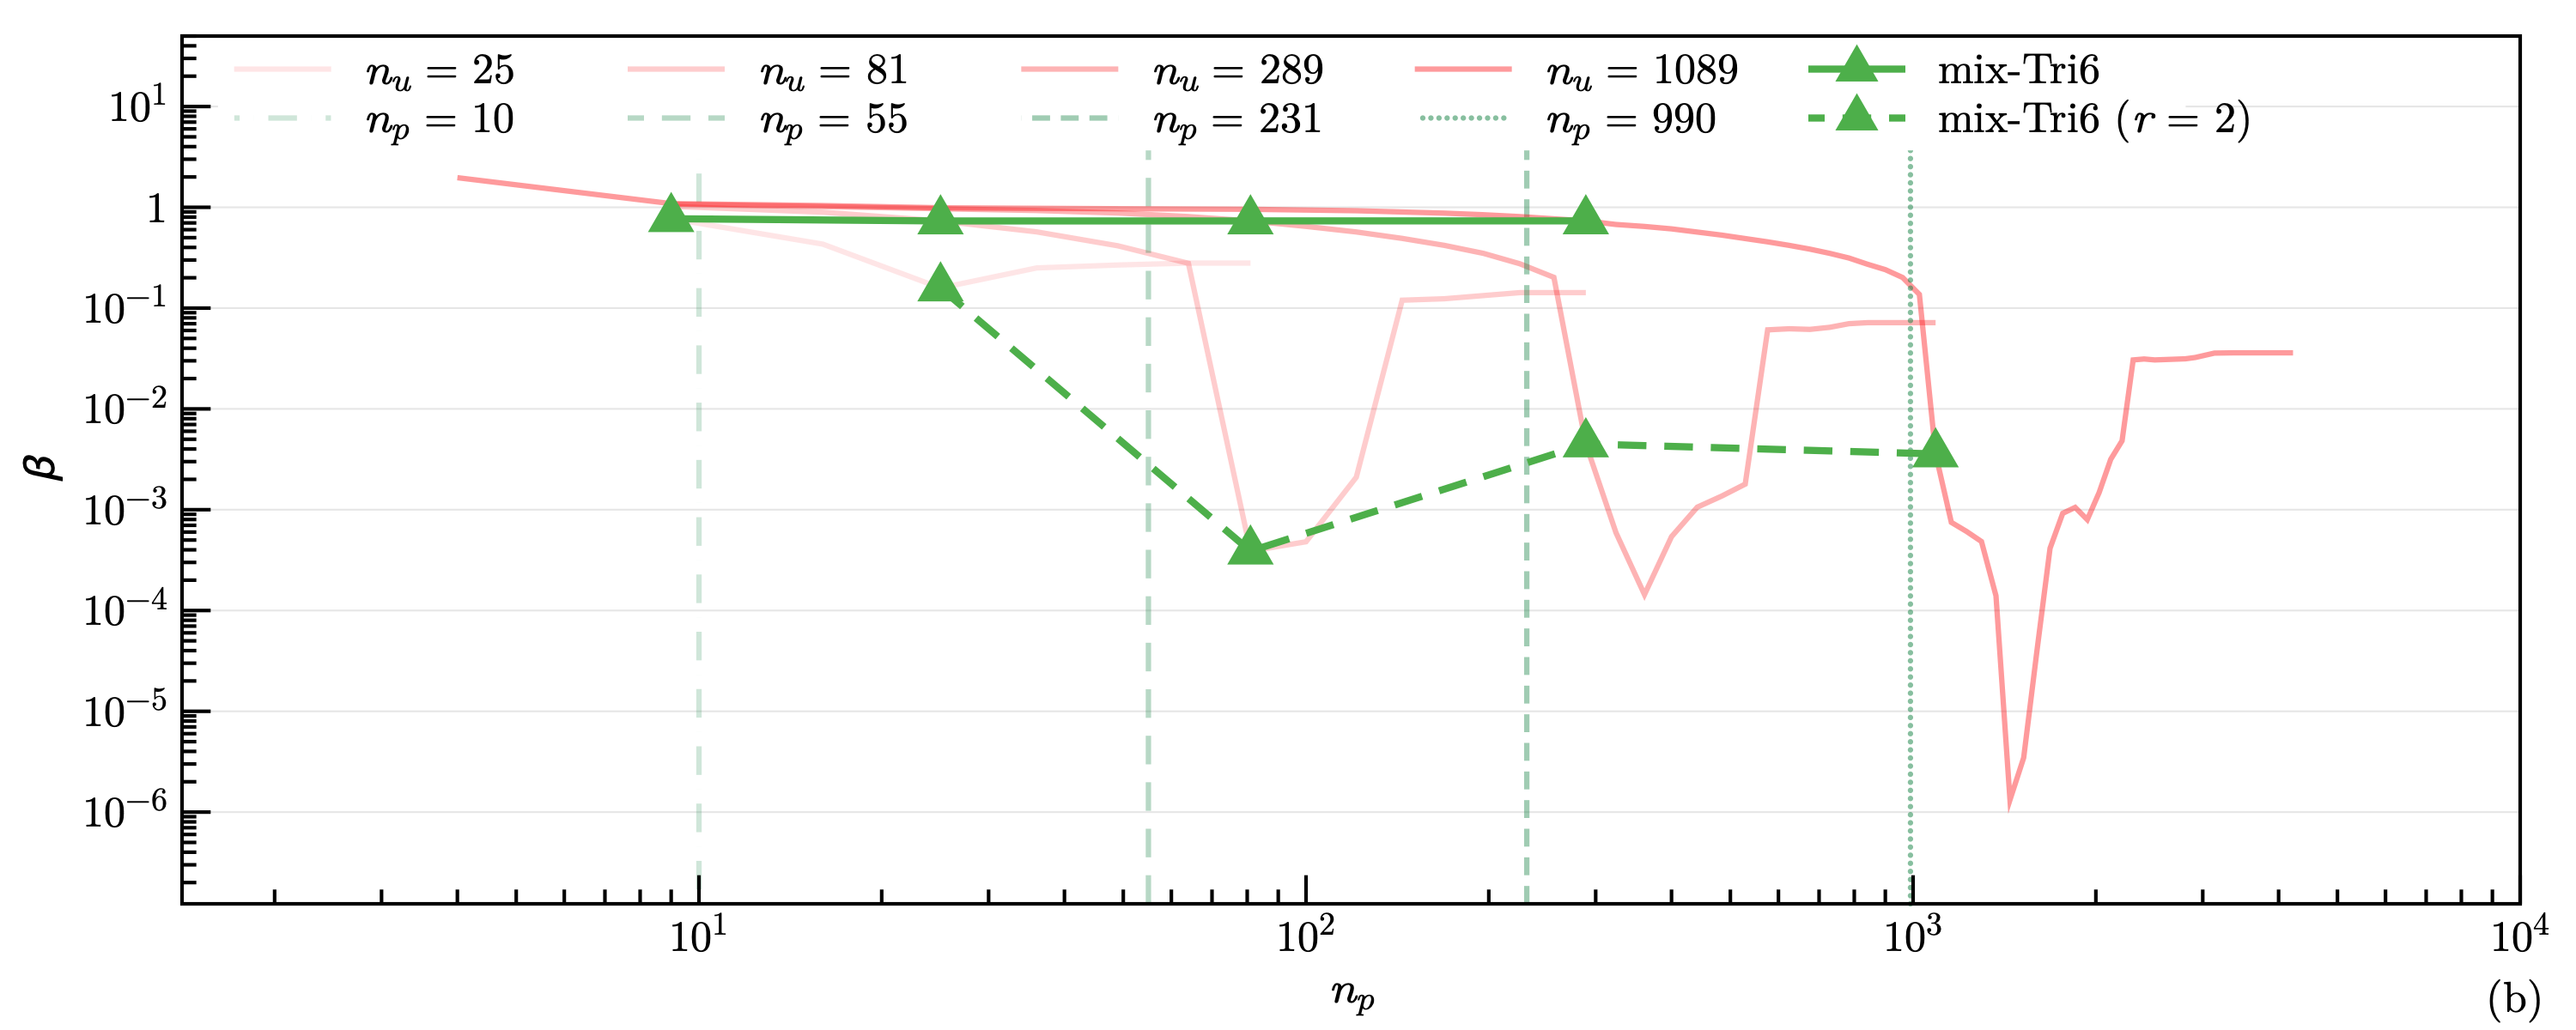
\includegraphics[width=0.9\textwidth]{figures/ch_4/infsup_tri6.png}\phantomcaption\label{b}
    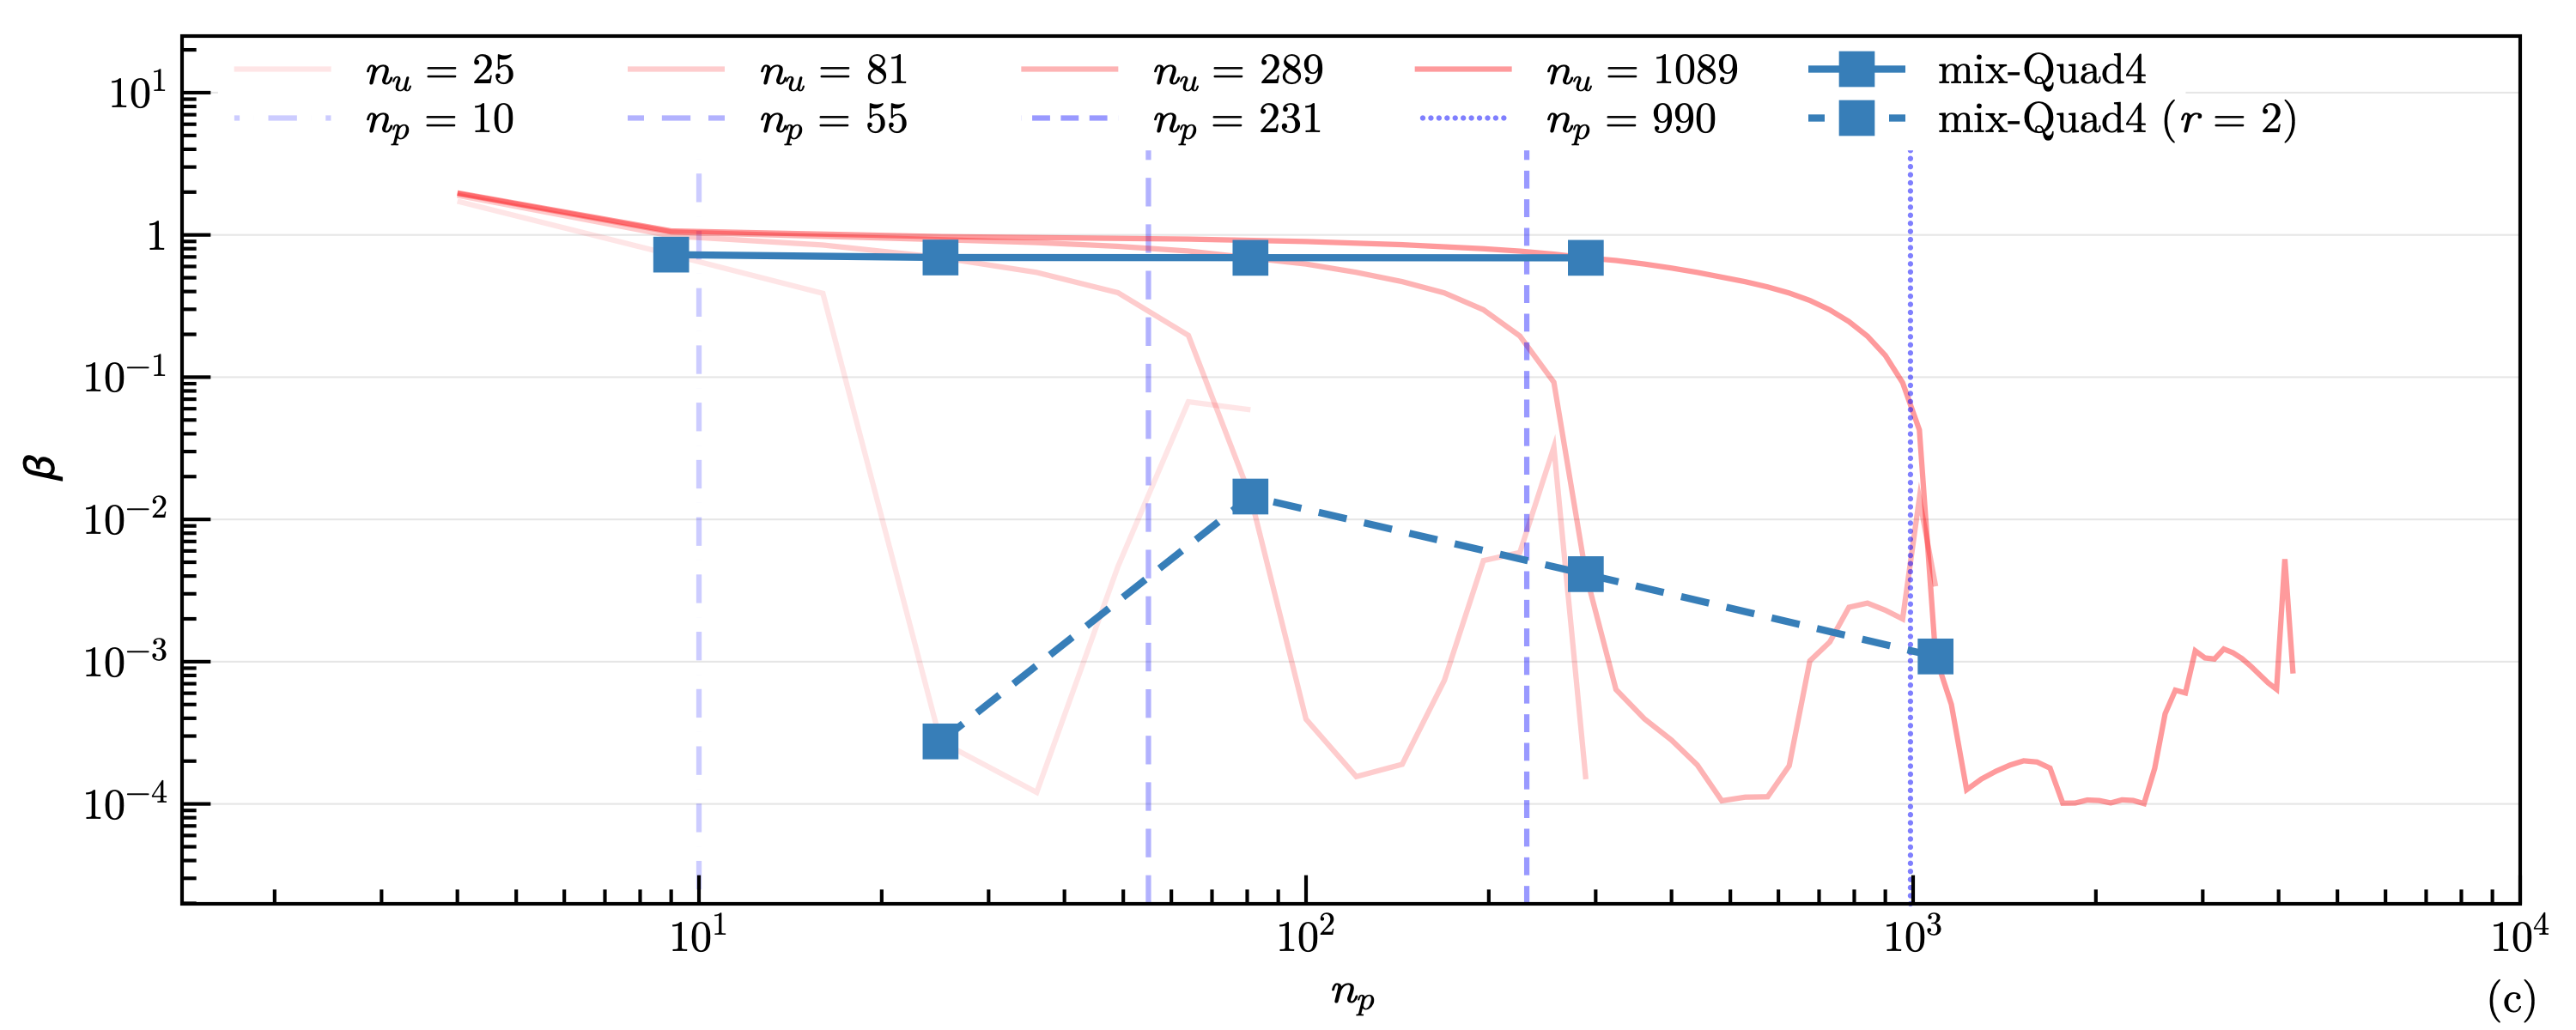
\includegraphics[width=0.9\textwidth]{figures/ch_4/infsup_quad.png}\phantomcaption\label{c}
    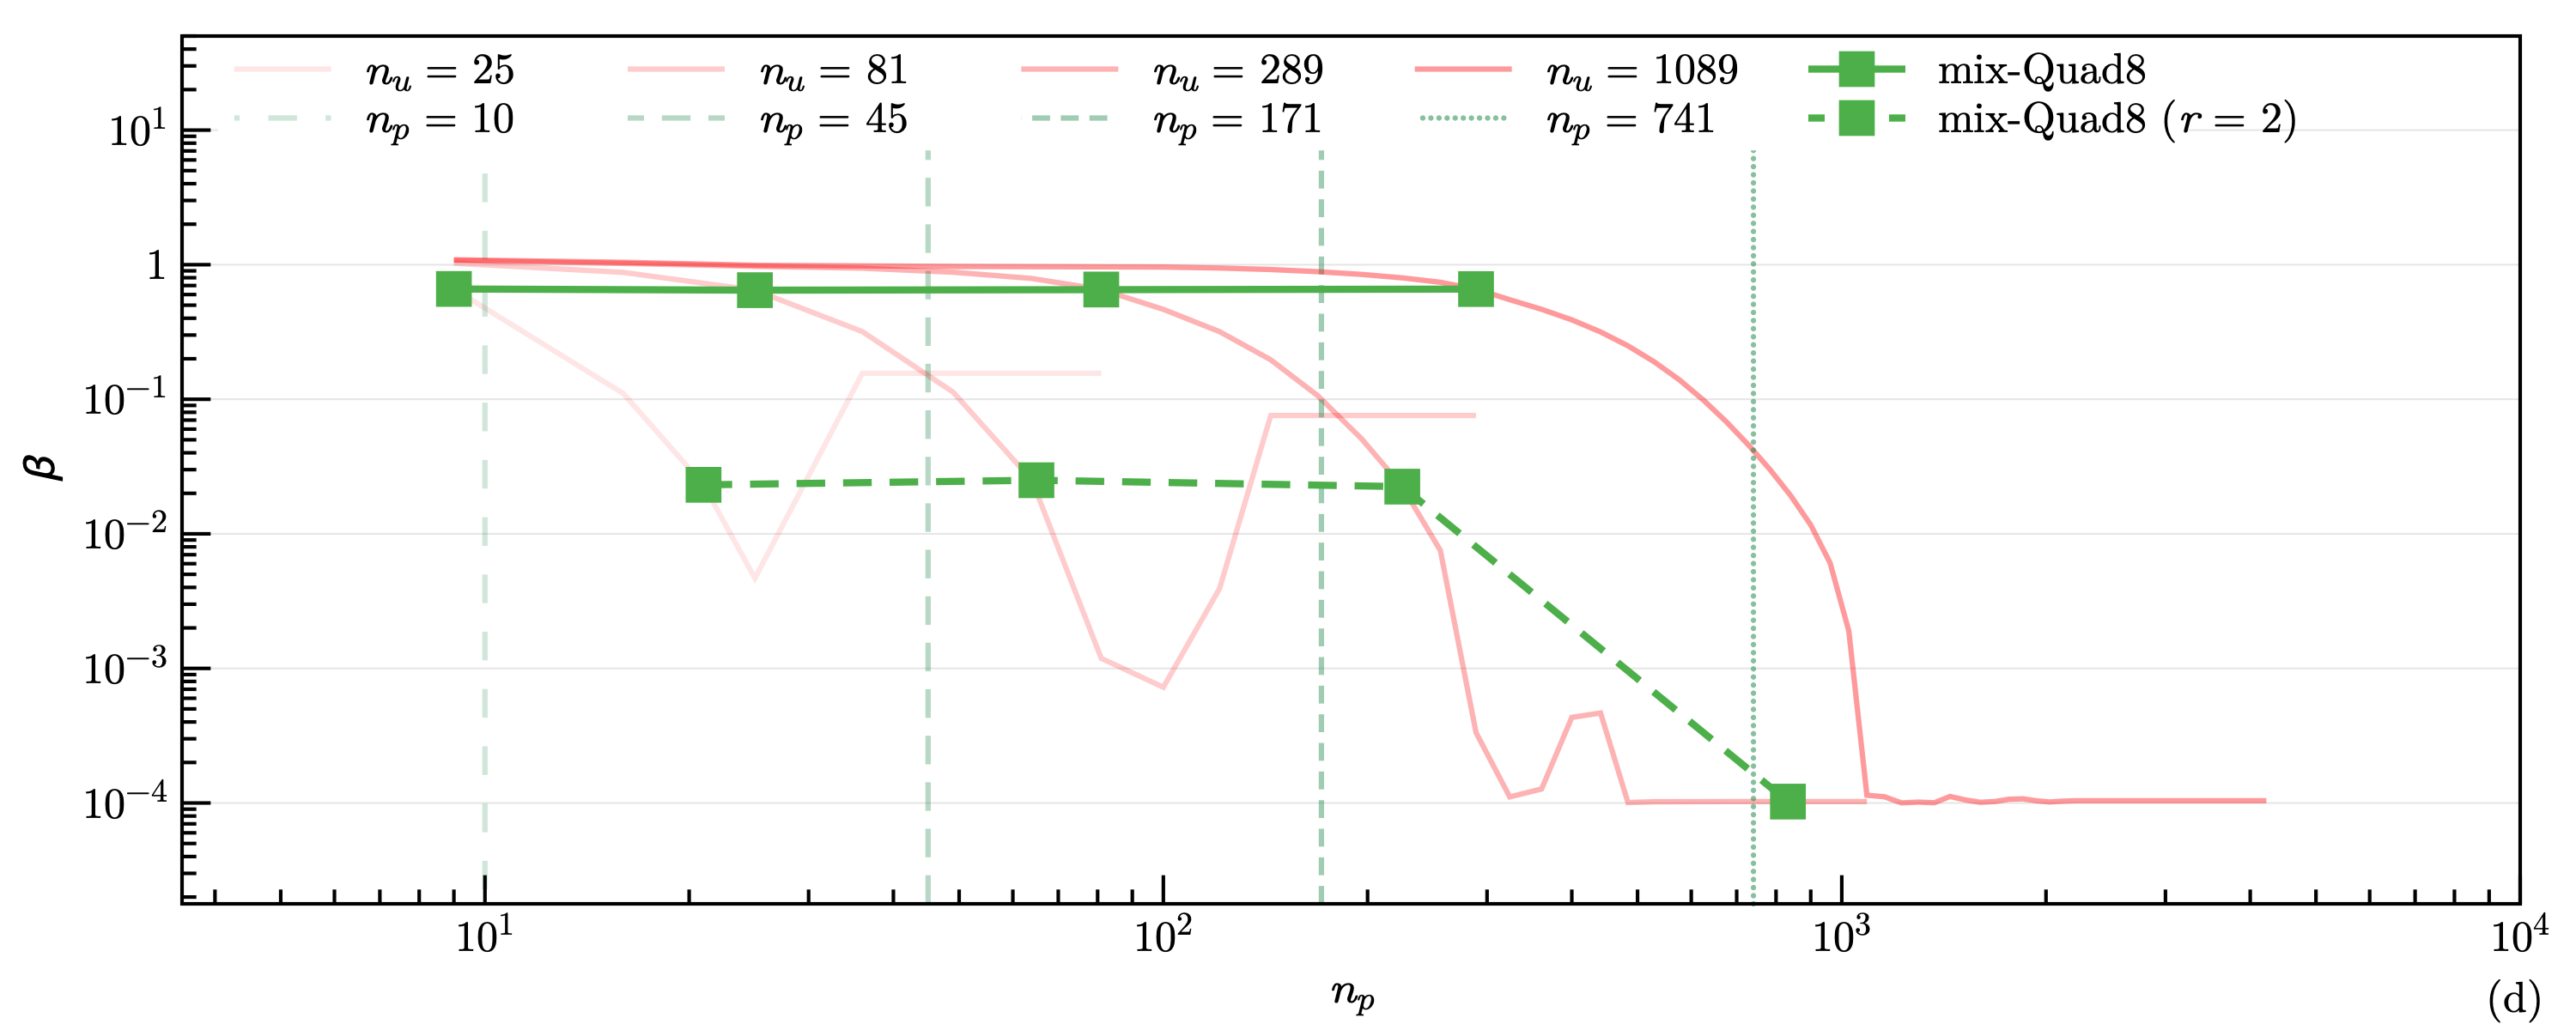
\includegraphics[width=0.9\textwidth]{figures/ch_4/infsup_quad8.png}\phantomcaption\label{d}
    \end{subcaptiongroup}
    \captionsetup{aboveskip=0pt}
    \caption{\centering 各种有限元方案的LBB稳定性条件测试 \\ \subref{a} mix-Tri3; \subref{b} mix-Tri6; \subref{c} mix-Quad4; \subref{d}mix-Quad8}\label{ch_4:fig:infsup_convergence}
\end{figure}

\begin{figure}[!ht]
    \centering
        \begin{tabular}{c@{\hspace{24pt}}c}
            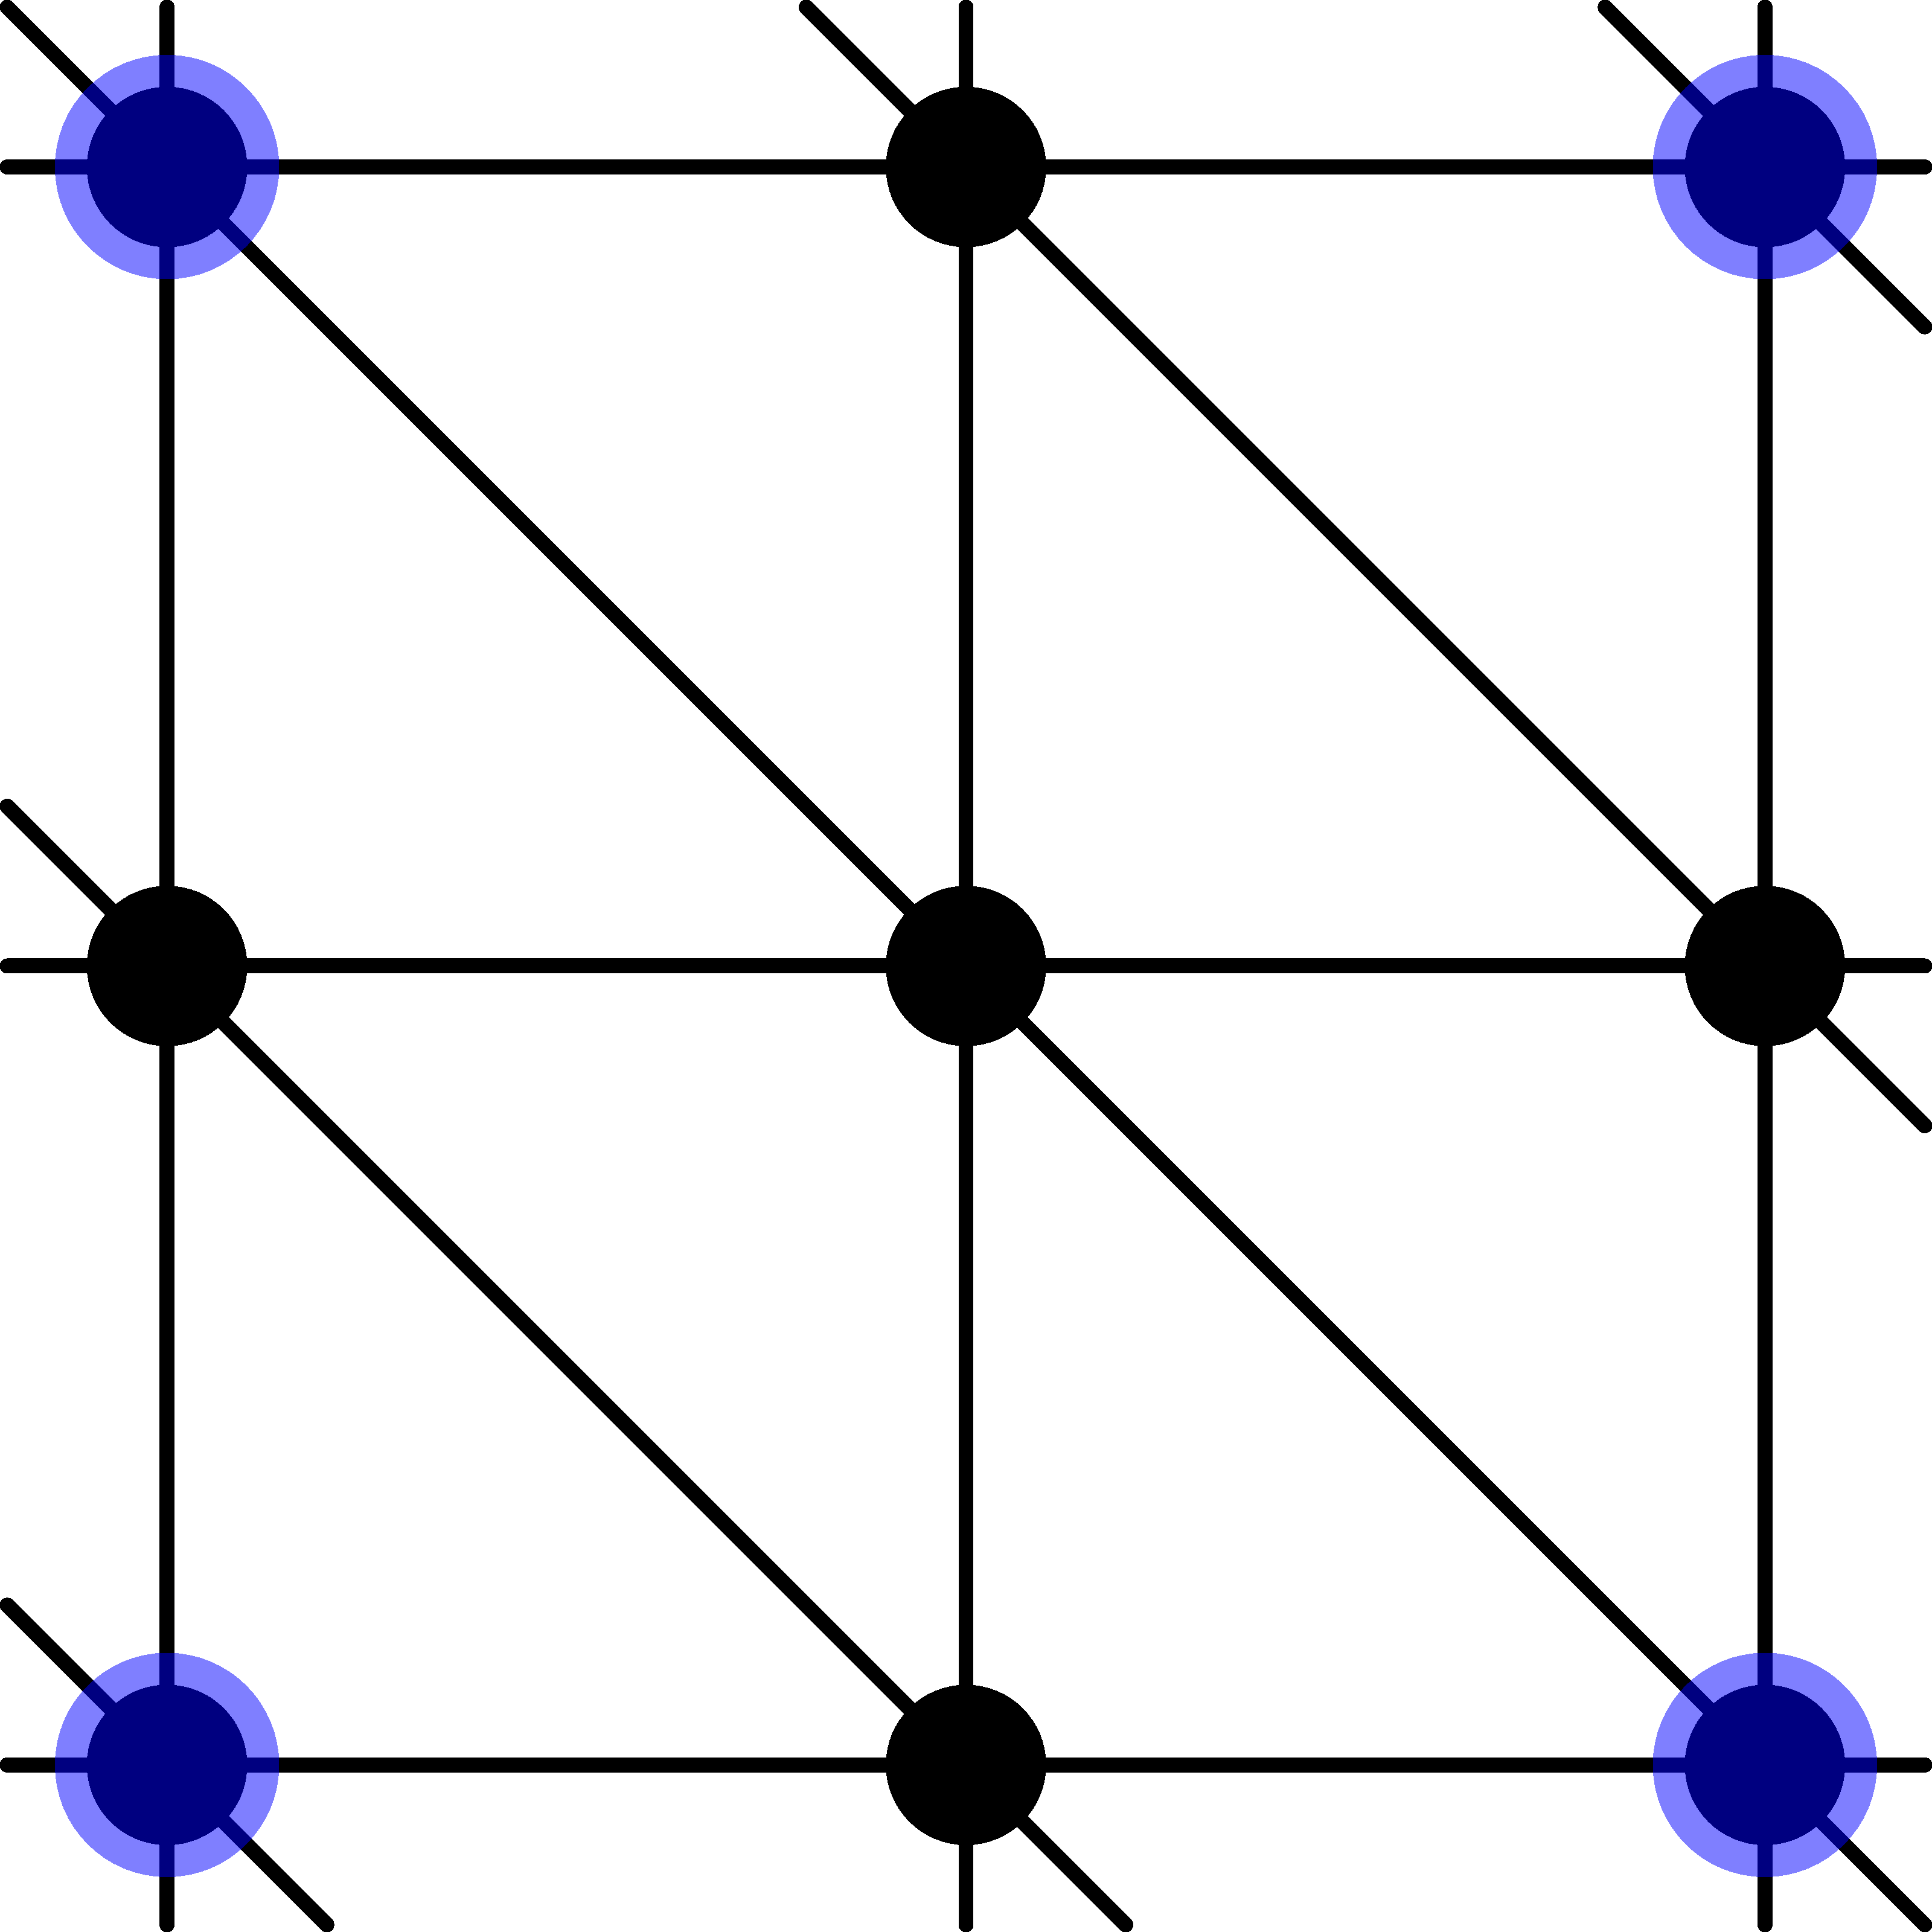
\includegraphics[width=0.3\textwidth]{figures/ch_4/mix_tri3.png} &
            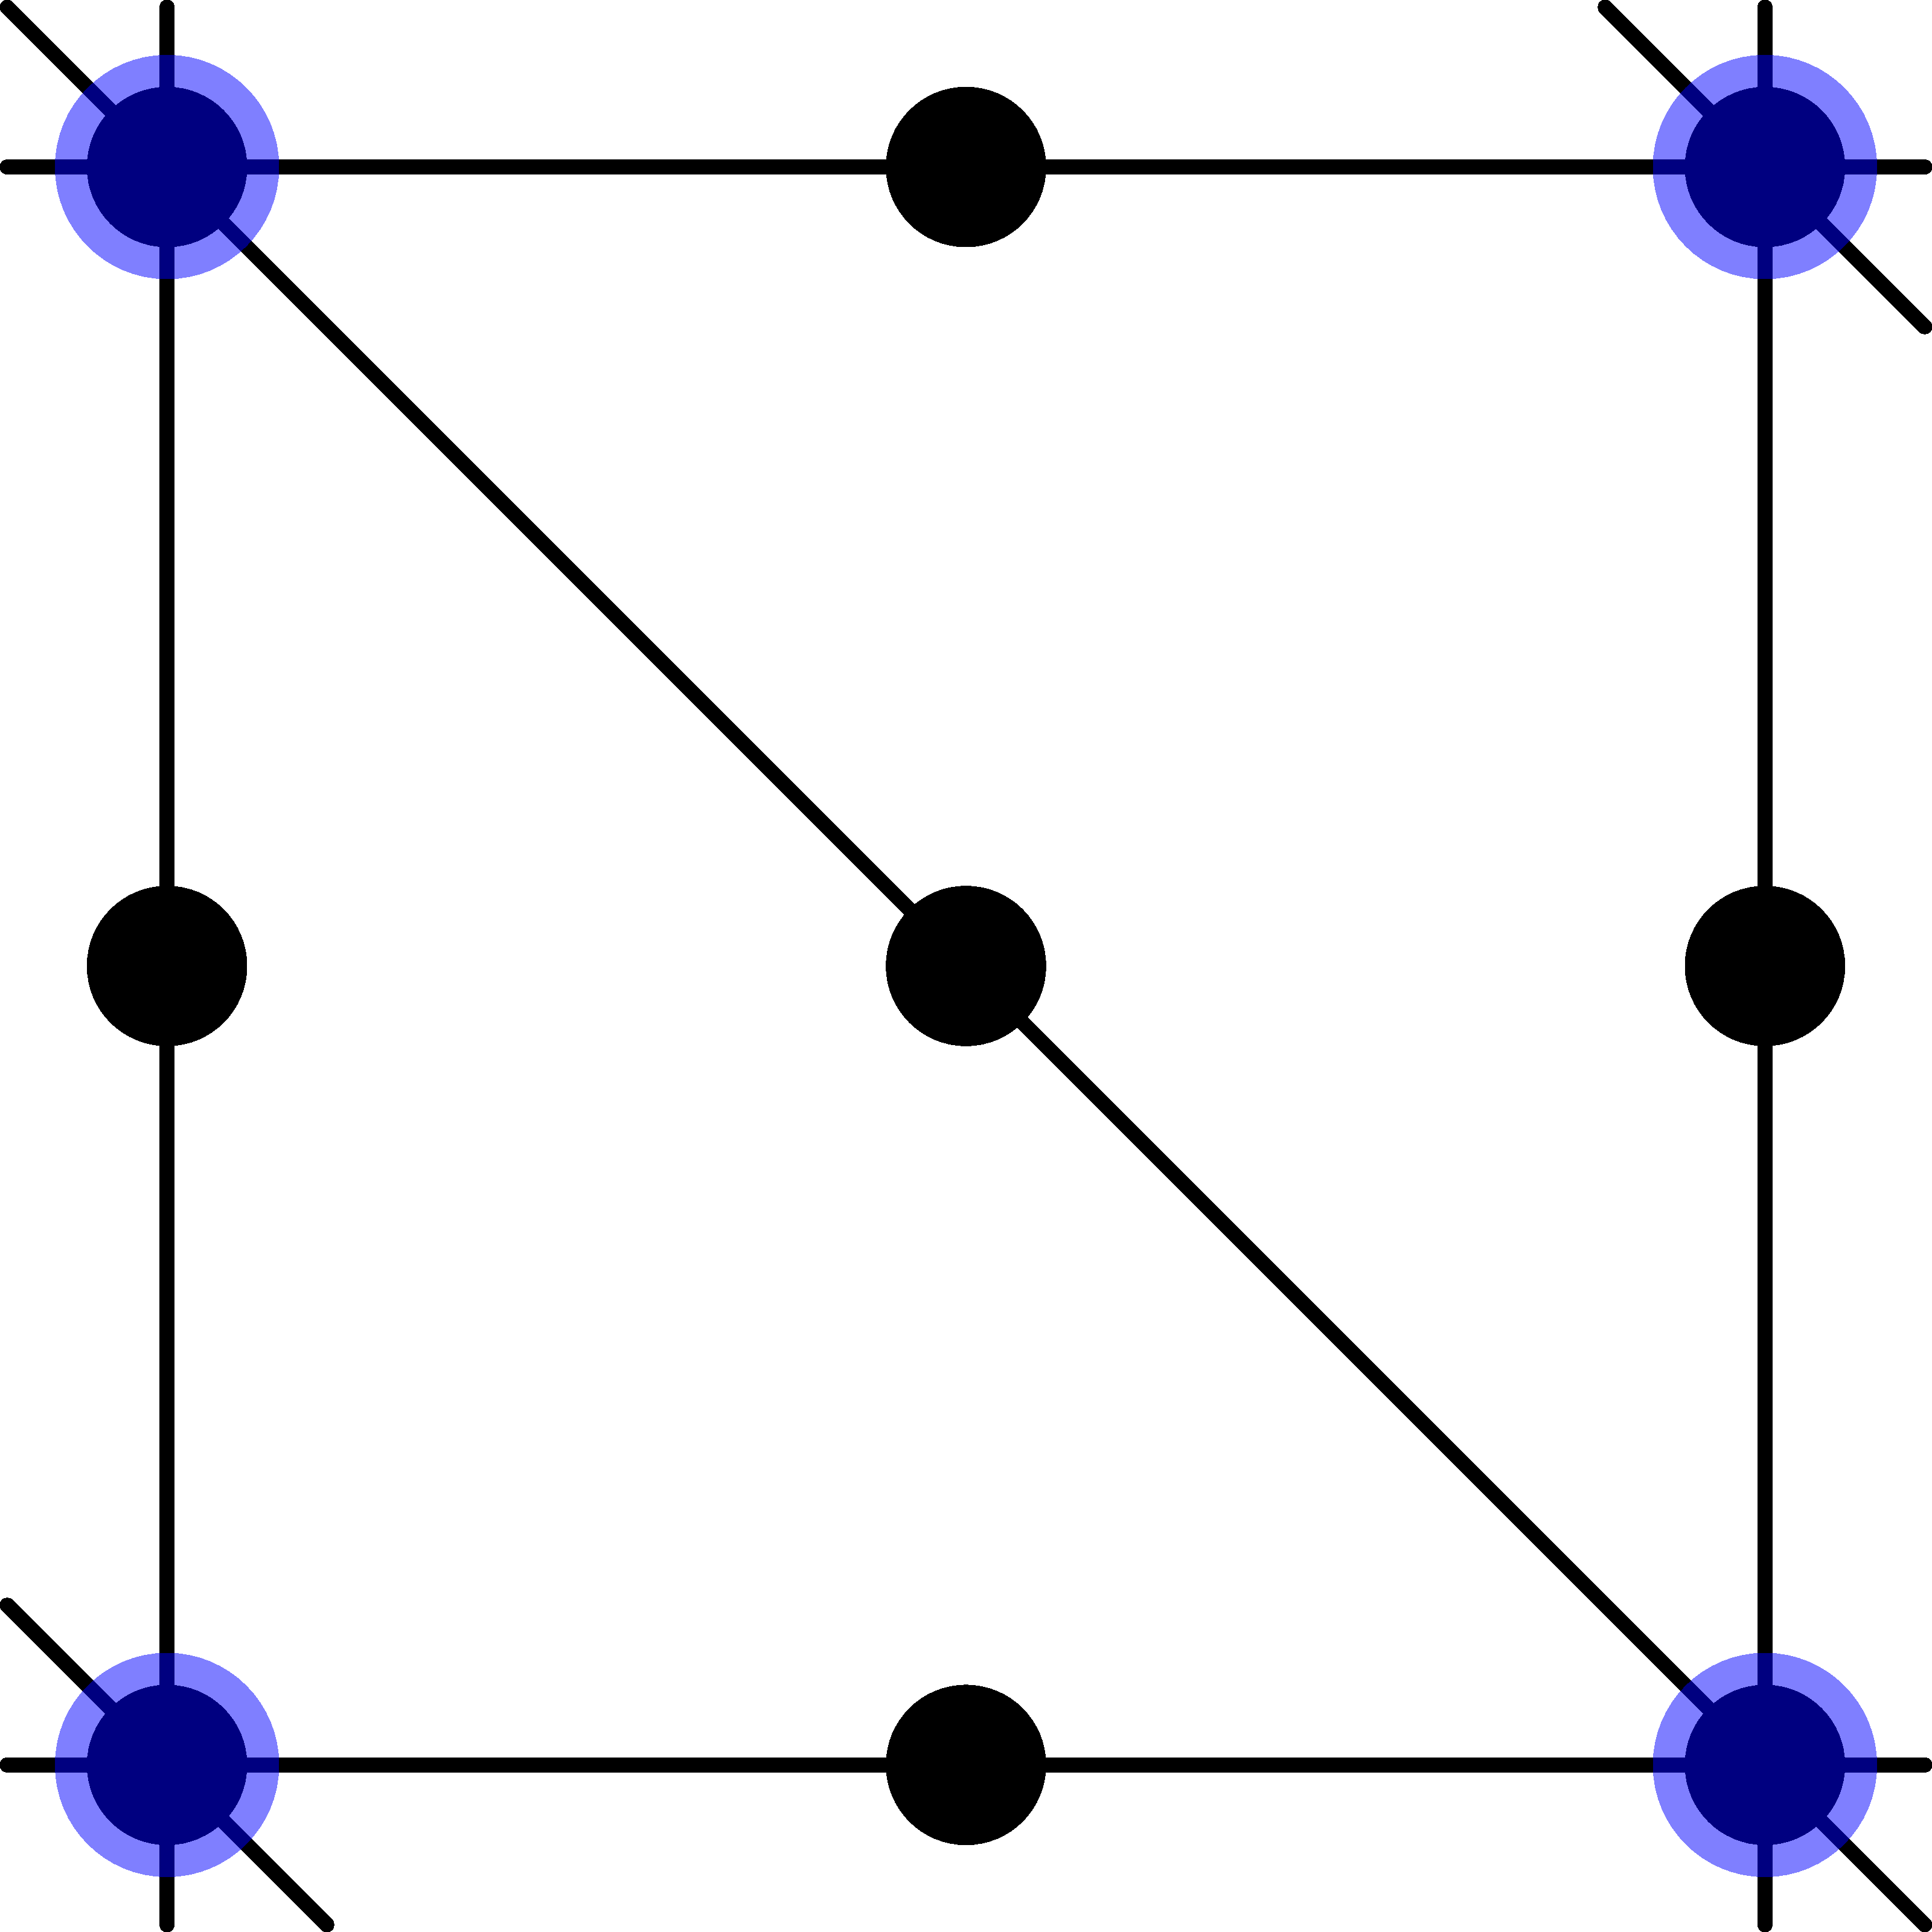
\includegraphics[width=0.3\textwidth]{figures/ch_4/mix_tri6.png} \\
            mix--Tri3 & mix--Tri6 \\
            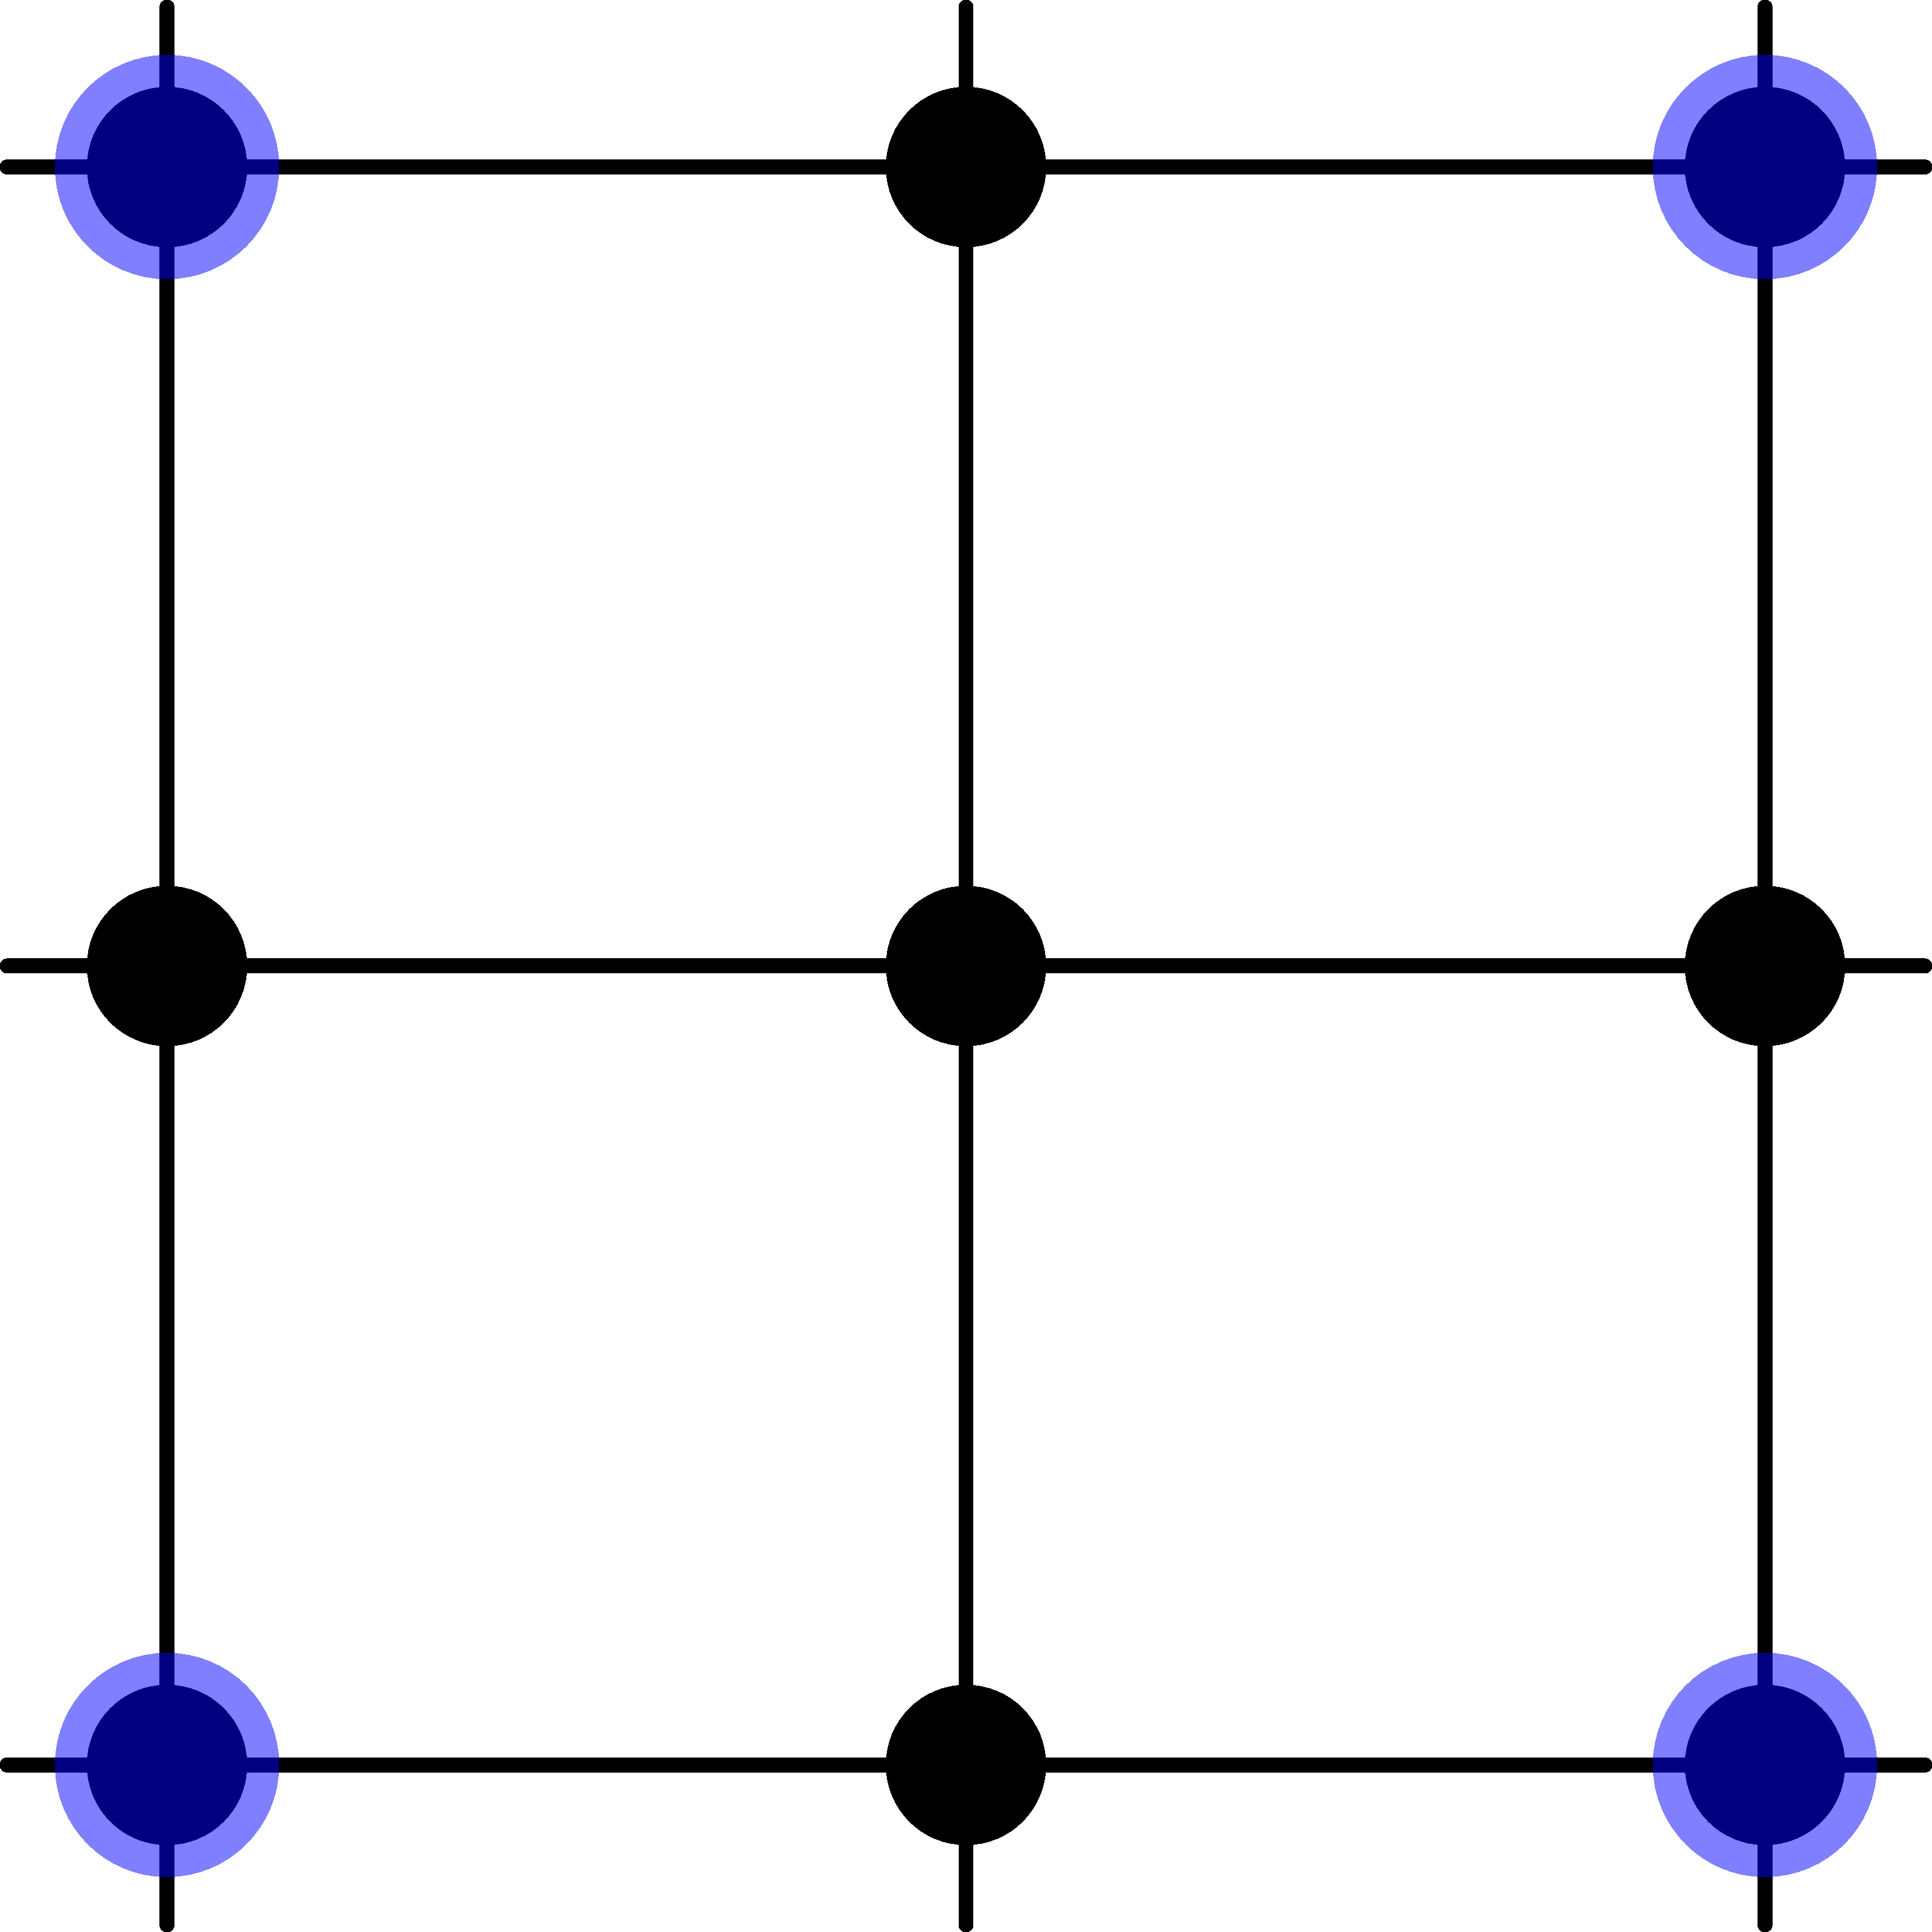
\includegraphics[width=0.3\textwidth]{figures/ch_4/mix_quad4.png} &
            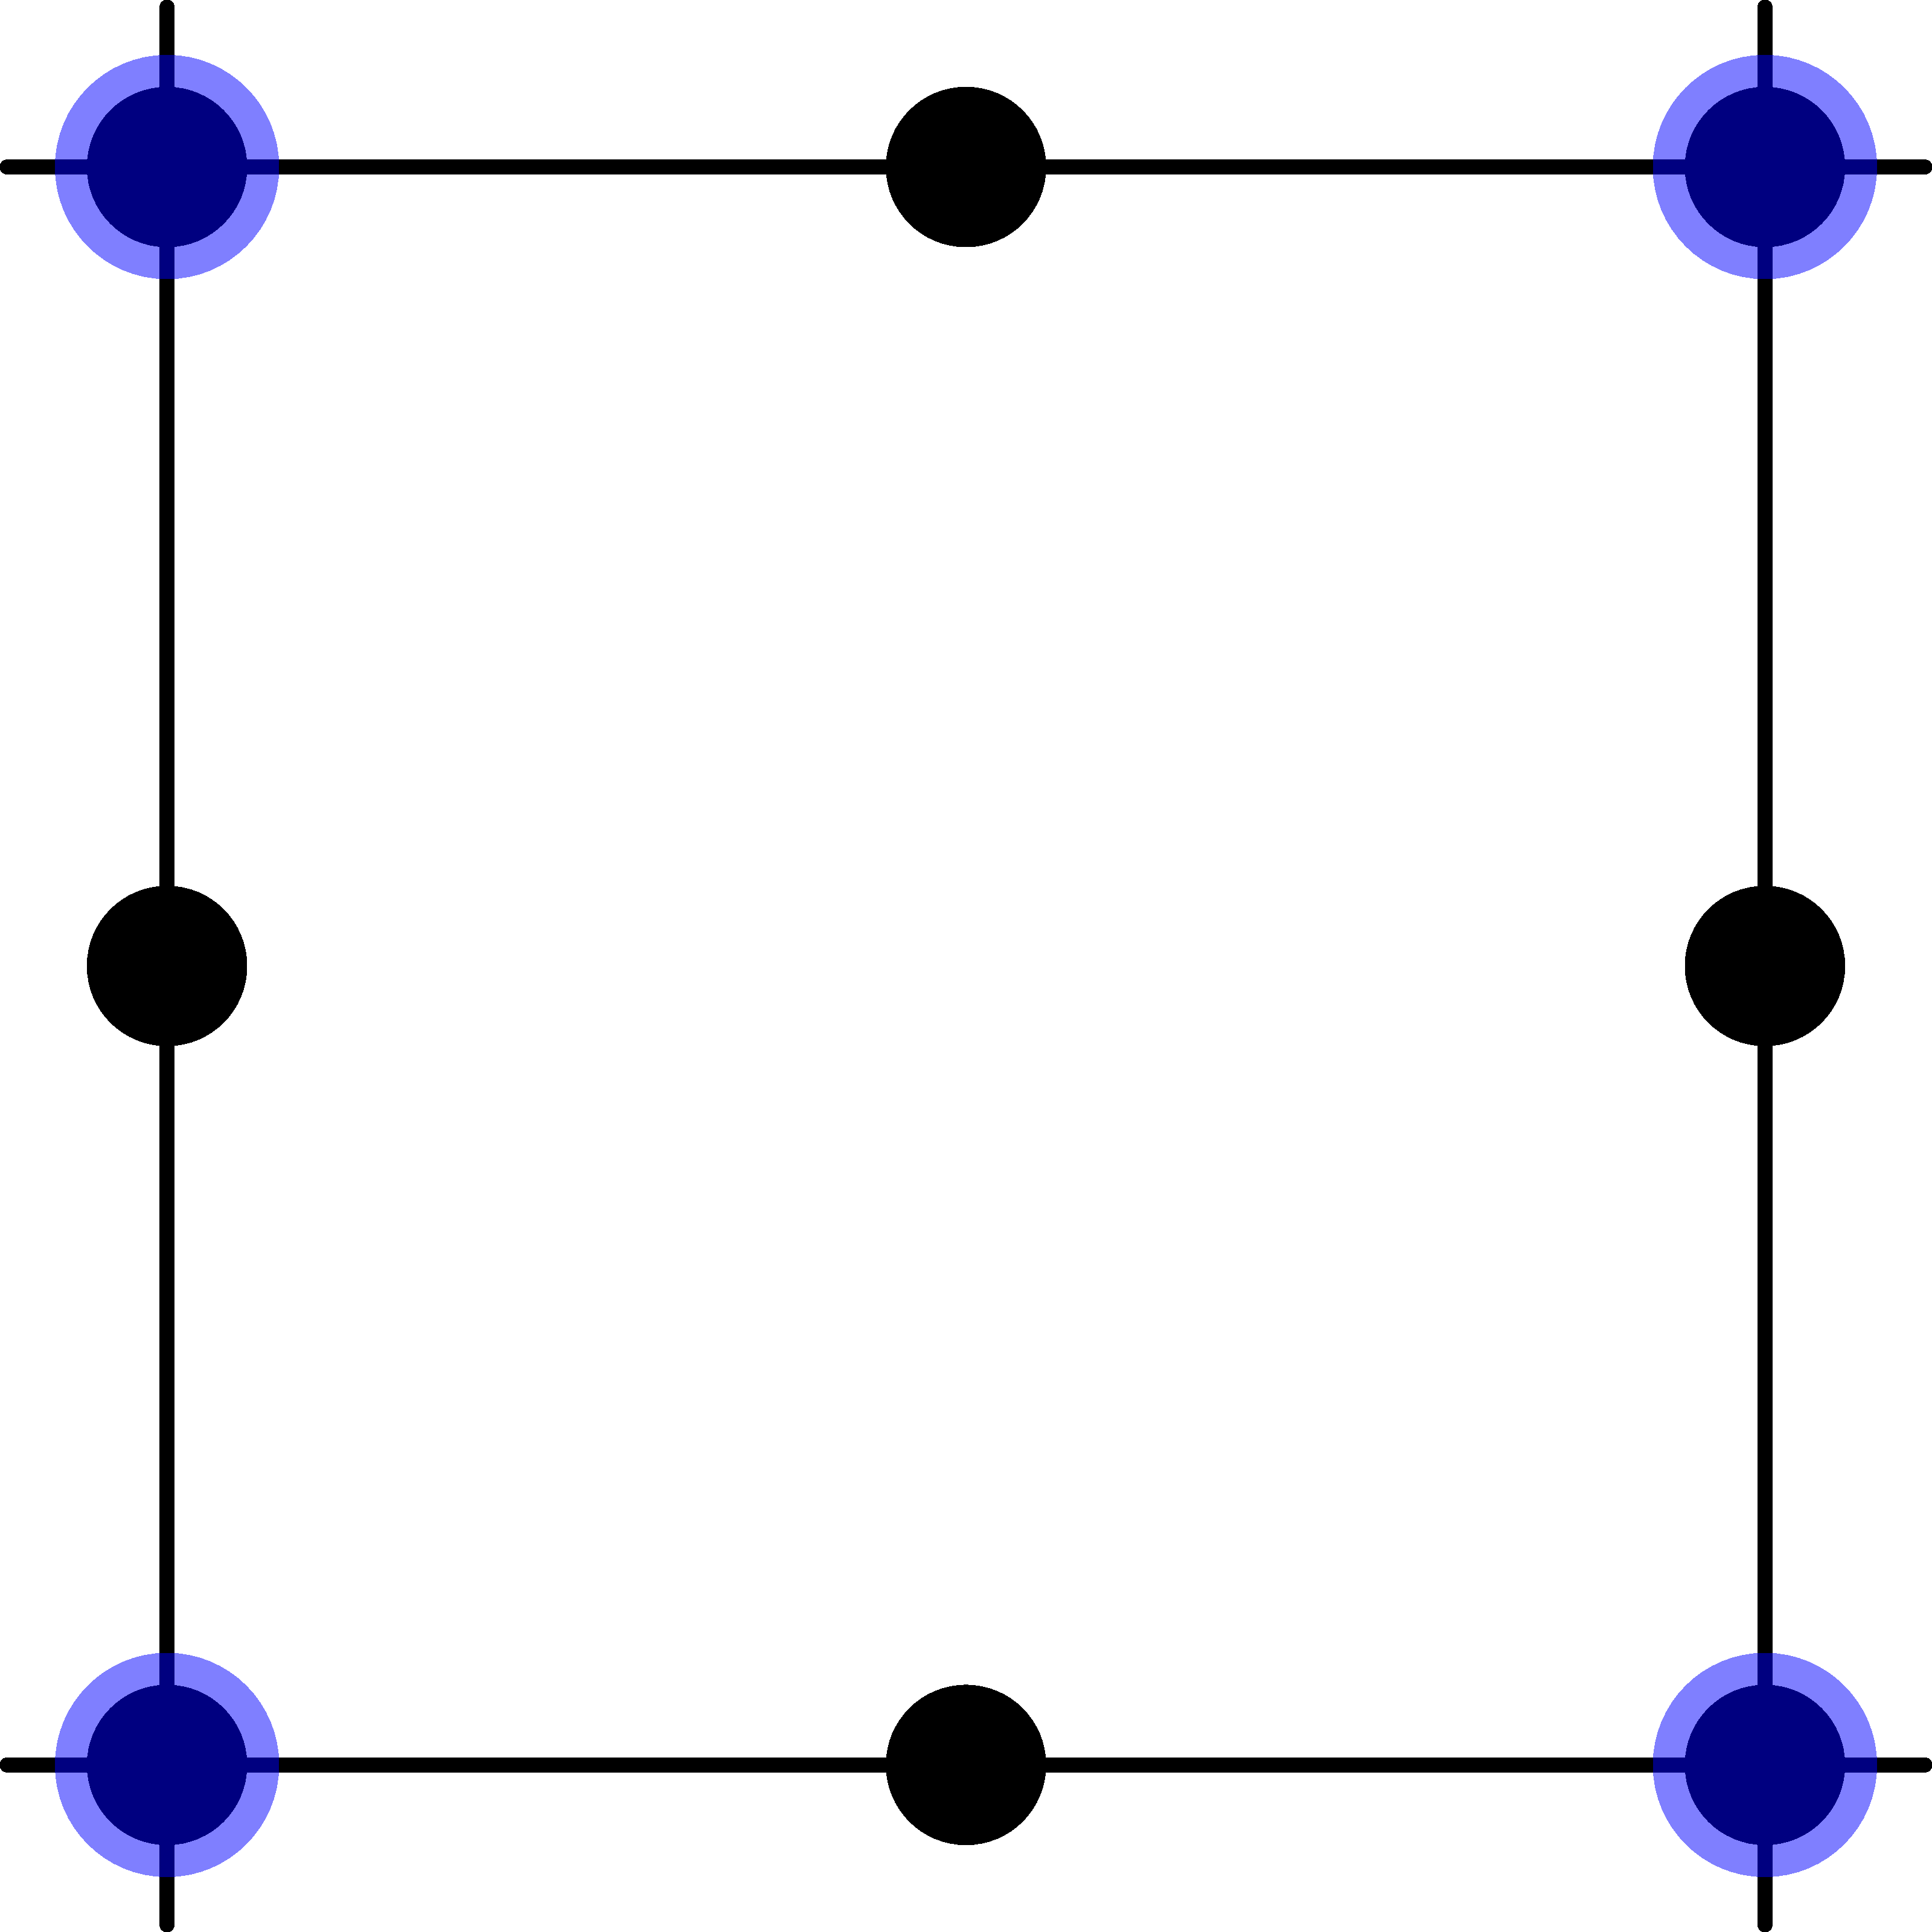
\includegraphics[width=0.3\textwidth]{figures/ch_4/mix_quad8.png} \\
            mix--Quad4 & mix--Quad8 \\
            \raisebox{-0.3\height}{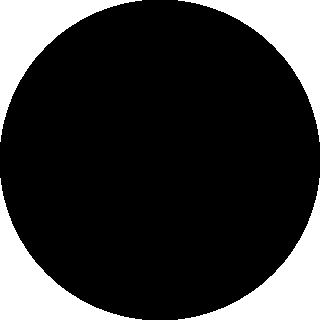
\includegraphics[width=14pt]{figures/legend_u.png}} :位移节点 &
            \raisebox{-0.3\height}{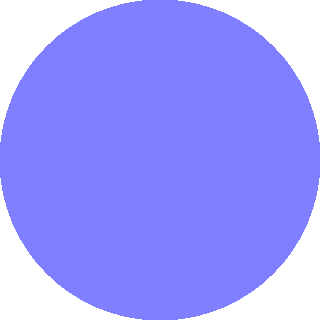
\includegraphics[width=14pt]{figures/legend_p.png}} :压力节点 
        \end{tabular}
        \caption{有限元无网格混合离散方案}\label{ch_4:fig:mix_scheme}
\end{figure}

\section{数值算例}
\subsection{悬臂梁问题}

首先考虑经典弹性力学二维悬臂梁问题,如图\ref{ch_4:fig:cantilever}所示,悬臂梁的长和宽分别为$L=48$,$D=12$,同时悬臂梁的左端为固定支座,
右端沿着$y$轴正方向施加外部荷载$P=1000$。悬臂梁的材料系数为杨氏模量$E=3\times10^6$、泊松比$\nu=0.5-10^{-8}$。
\begin{figure}[!h]
    \centering 
        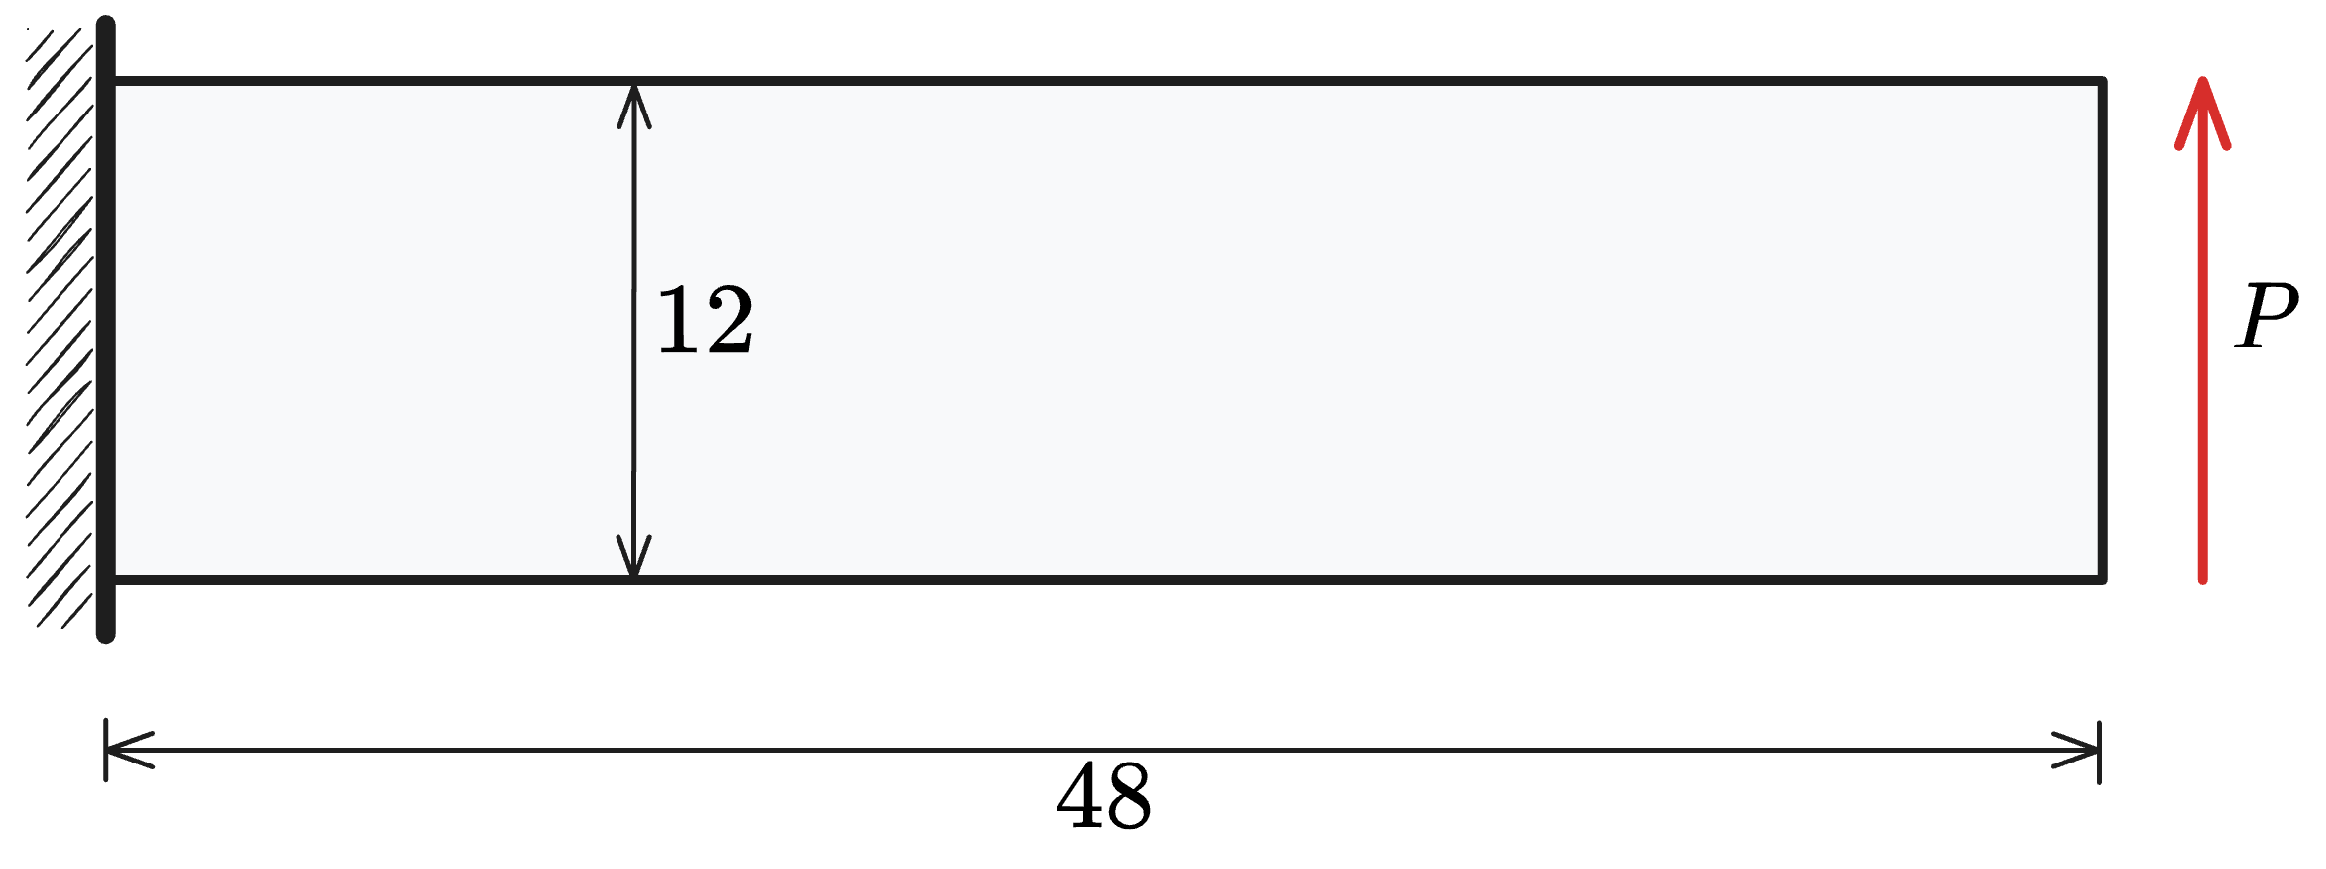
\includegraphics[scale=0.4]{figures/ch_4/cantilever.png}
        \caption{悬臂梁问题模型}\label{ch_4:fig:cantilever}
\end{figure}

根据圣维南原理和平面应力假设,悬臂梁问题的解析解为:
\begin{equation}
    \begin{split}
        u_1 &= -\frac{Py}{6EI}[(6L-3x)x + (2+\nu)(y^2 - \frac{D^2}{4})] \\
        u_2 &= \frac{P}{6EI}[3\nu y^2(L-x) + (4+5\nu)\frac{D^2x}{4} + (3L-x)x^2]
    \end{split}
\end{equation}
与之相对应的应力分量为:
\begin{equation}
       \sigma_{xx}=-\frac{P(L-x)y}{I},\,\sigma_{yy}=0,\,\sigma_{xy}=\frac{P}{2I}(\frac{D^2}{4}-y^2)
\end{equation}

选取Quad4和Quad8两种离散单元,分别四个不同数量的位移节点数$n_u$进行分析,以验证在$n_u$固定的情况下,压力节点数$n_p$与位移误差和压力误差的关系。图\ref{ch_4:fig:cantilever_2}展示了相应的分析结果,其中虚线表示LBB稳定系数估计的最优约束比下的压力节点数量。
从图中可以观察到以下规律:由于二次单元Quad8的高阶插值特性,其本身就具有一定缓解自锁的特性,压力节点数$n_p$的变化对位移误差的影响几乎可以忽略;而对于线性单元Quad4,随着$n_p$的逐渐减少,位移误差也呈现减小的趋势,并在达到最优$n_p$时位移误差也达到最小值。值得注意的是,当$n_p$小于最优值时,位移误差仍然保持在较低水平。类似的现象也体现在压力误差的分析中,且随着网格密度的增加,这一趋势更加明显密。
上述结果表明,当压力节点数$n_p$小于最优值时,离散方案能获得高精度的位移解和压力解。

图\ref{ch_4:fig:cantilever_P}为悬臂梁问题的压力云图。图(a),(b)为Quad4单元的压力云图,其中图(a)传统混合离散方案出现了明显的压力振荡现象,而图(b)本文提出的离散方案则没有出现压力振荡现象,表现出更好的数值稳定性。图(c),(d)为Quad8单元的压力云图,图(c)为LBB误差估计推出的最优约束比的离散方案,图中仍存在一定的压力振荡现象;相比之下,图(d)所提离散方案则完全没有压力振荡现象。这些结果进一步验证了本文所提离散方案能够获得高精度的压力解,同时有效消除了压力振荡现象。

图\ref{ch_4:fig:cantileve_l2}为悬臂梁问题Quad4和Quad8单元的位移误差和压力误差对比图。从图中可以明显看出:对于位移误差,Quad4单元的传统混合离散方案无法达到理论误差收敛率,而本文所提的离散方案可以达到理论误差收敛率;对于Quad8单元,两种离散方案均能达到理论误差收敛率。对于压力误差,无论是Quad4单元还是Quad8单元,传统混合离散方案均无法达到理论误差收敛率,而本文所提方案则能够达到理论误差收敛率。这些结果进一步验证了本文所提离散方案具有很好的数值精度和稳定性。
\begin{figure}[H]
    \centering
    \begin{subcaptiongroup}
        \begin{tabular}{c@{\hspace{0pt}}c@{\hspace{0pt}}c}
          $\Vert \boldsymbol u - \boldsymbol u_h \Vert_V$ & $\Vert p - p_h \Vert_Q$ &$n_u$ \\
          \raisebox{-0.8\height}{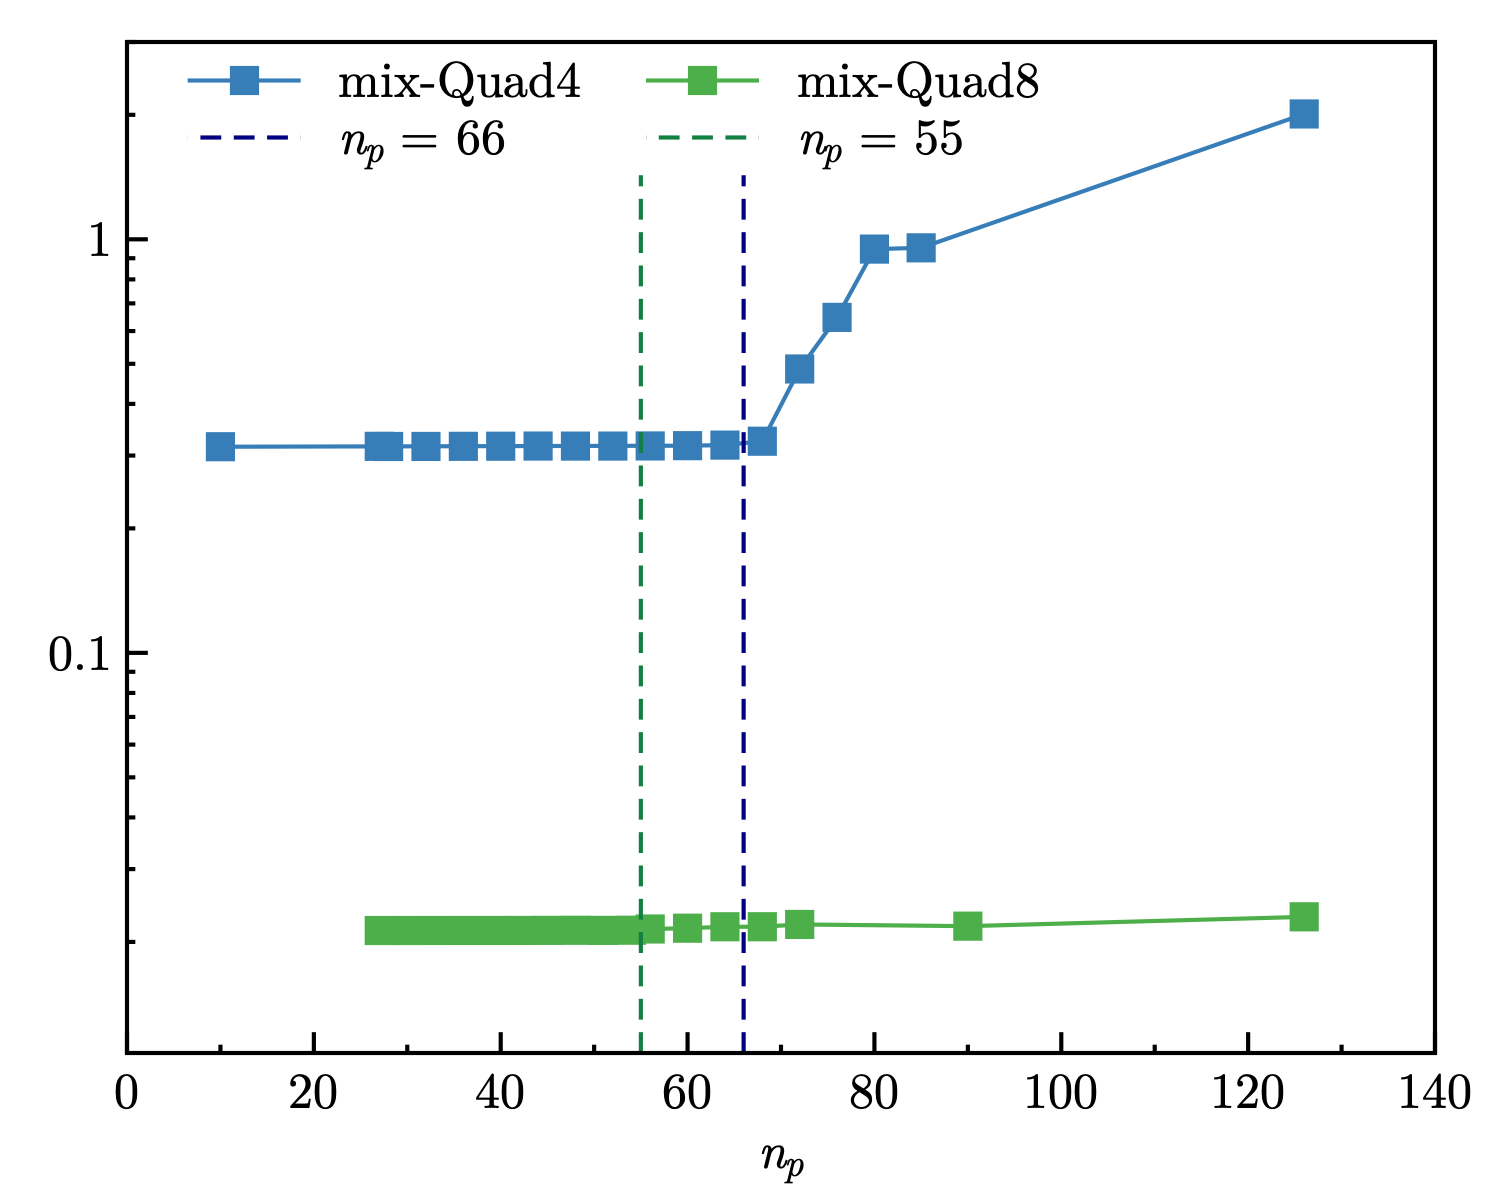
\includegraphics[width=0.45\textwidth]{figures/ch_4/cantilever_Hdev_4.png}}
        & \raisebox{-0.8\height}{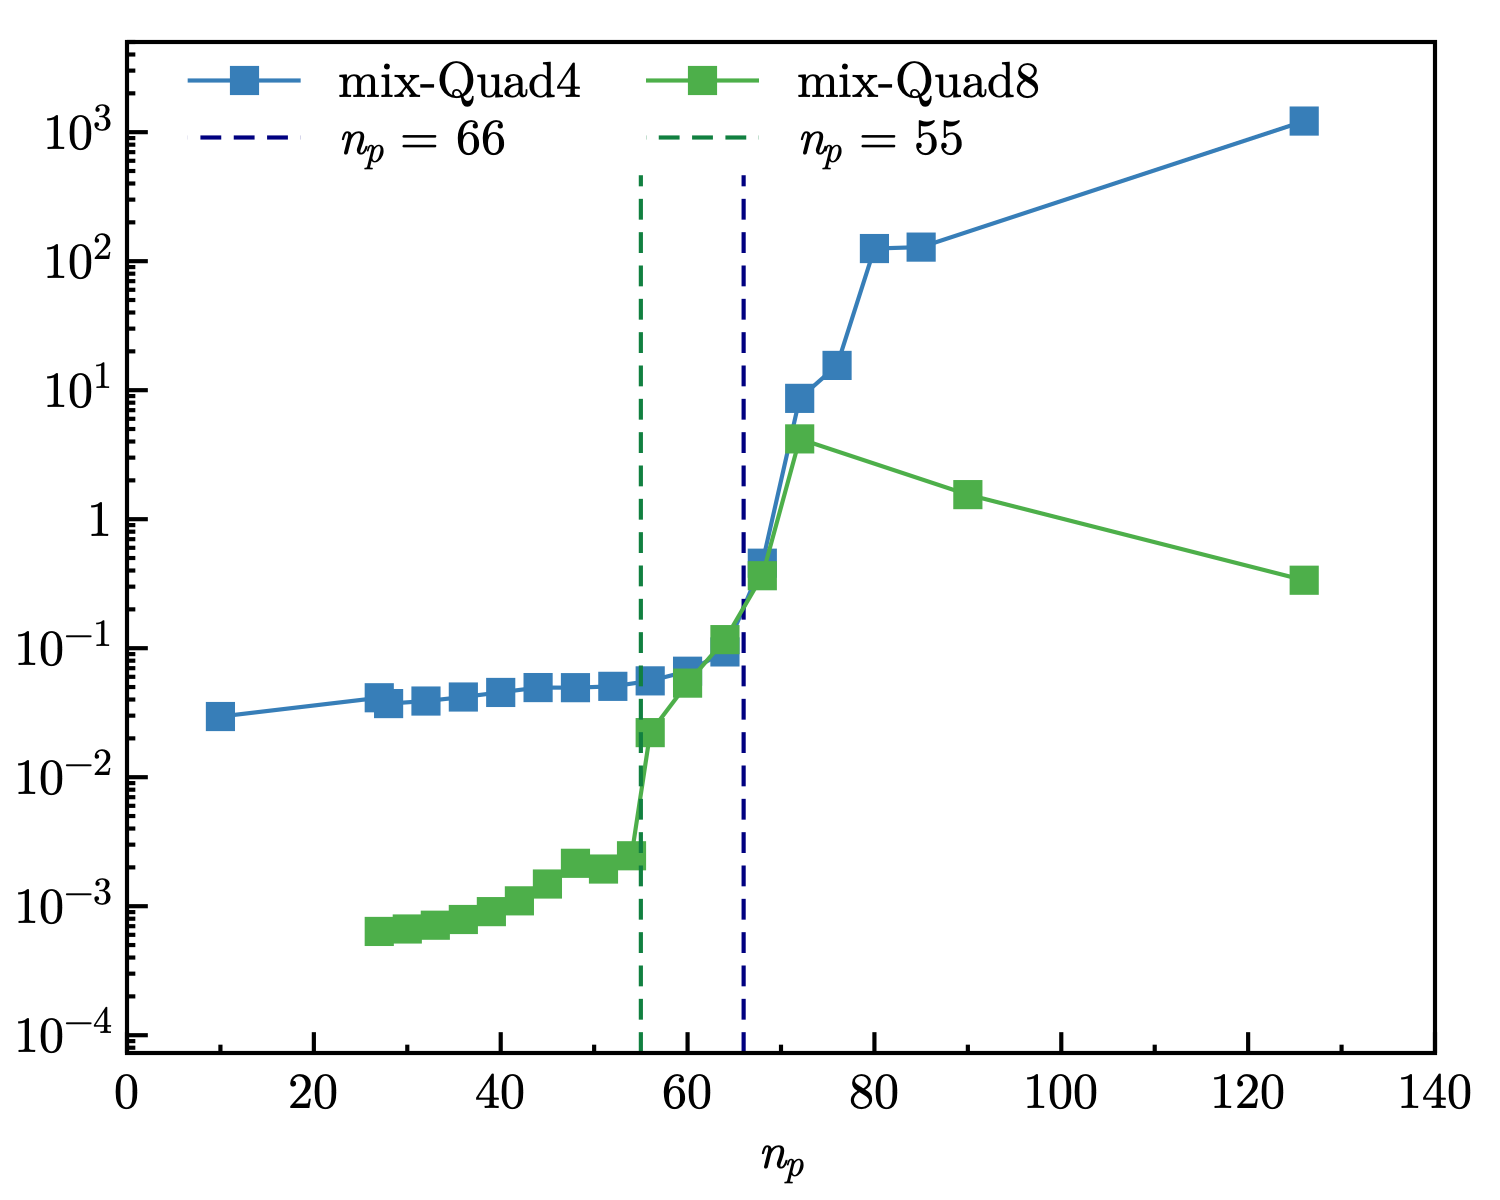
\includegraphics[width=0.45\textwidth]{figures/ch_4/cantilever_L2_p_4.png}}
        & \rotatebox{-90}{\parbox[b]{4cm}{Quad4: 85 nodes \\ Quad8: 80 nodes}} \\
          \raisebox{-0.85\height}{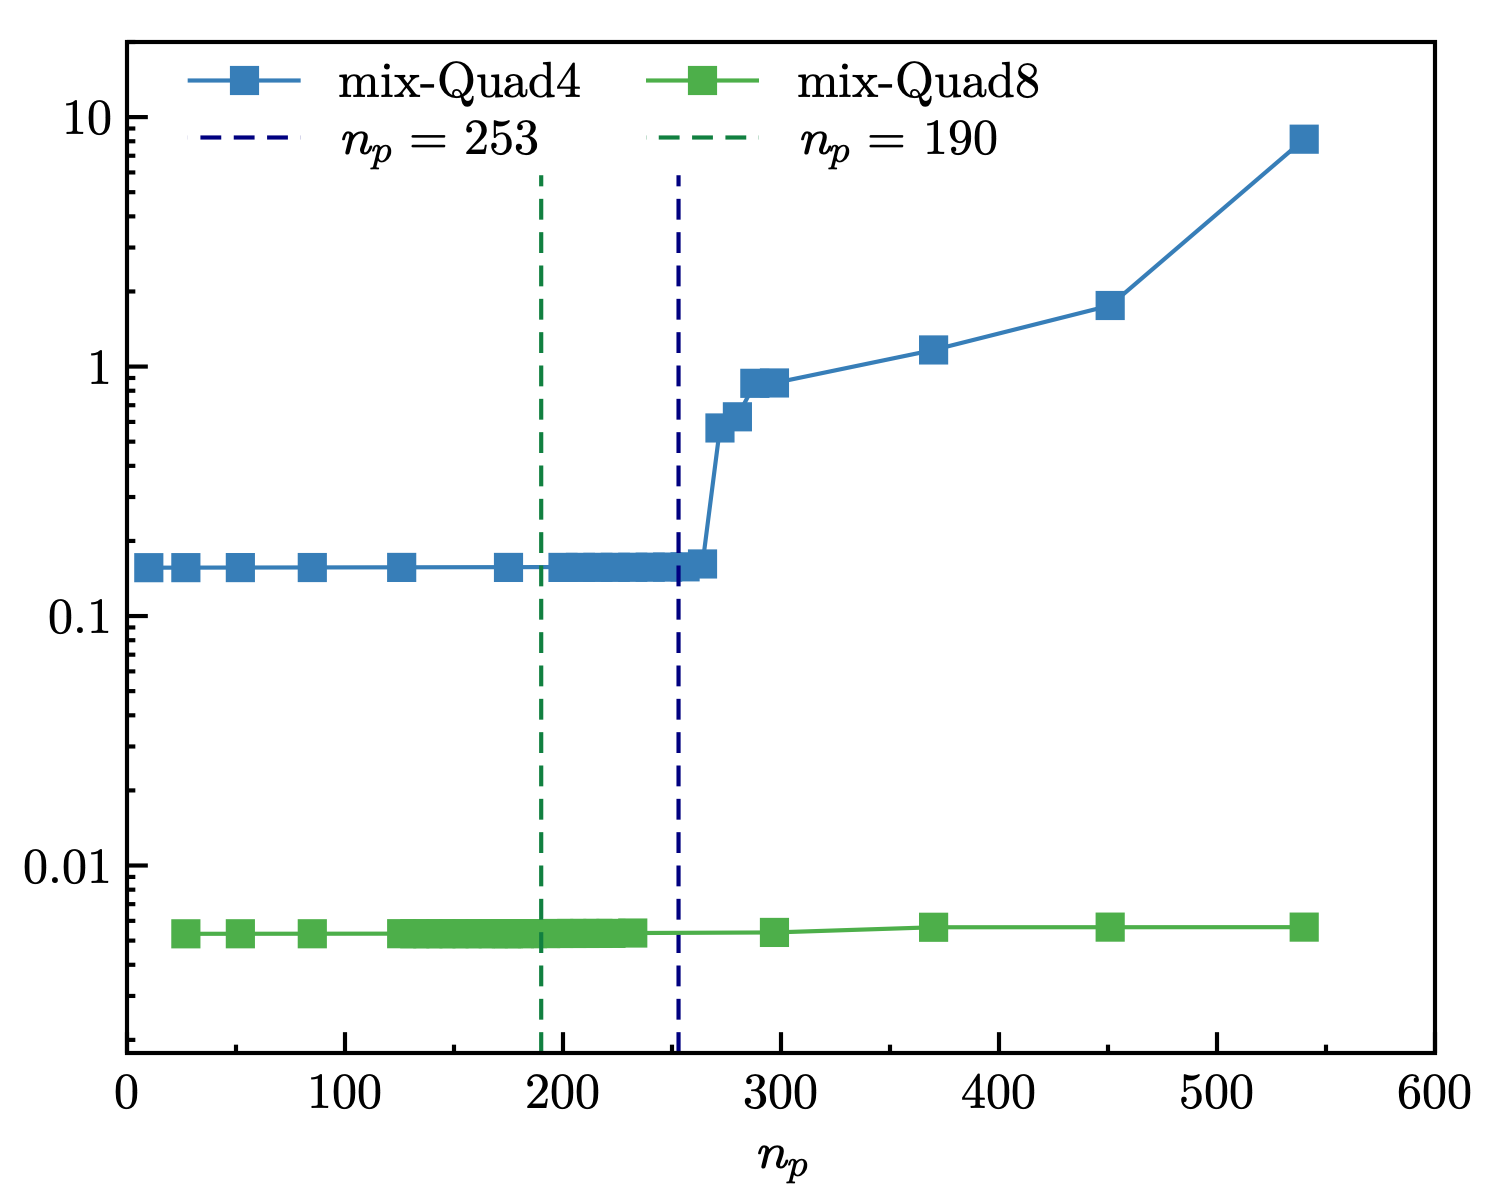
\includegraphics[width=0.45\textwidth]{figures/ch_4/cantilever_Hdev_8.png}}
        & \raisebox{-0.85\height}{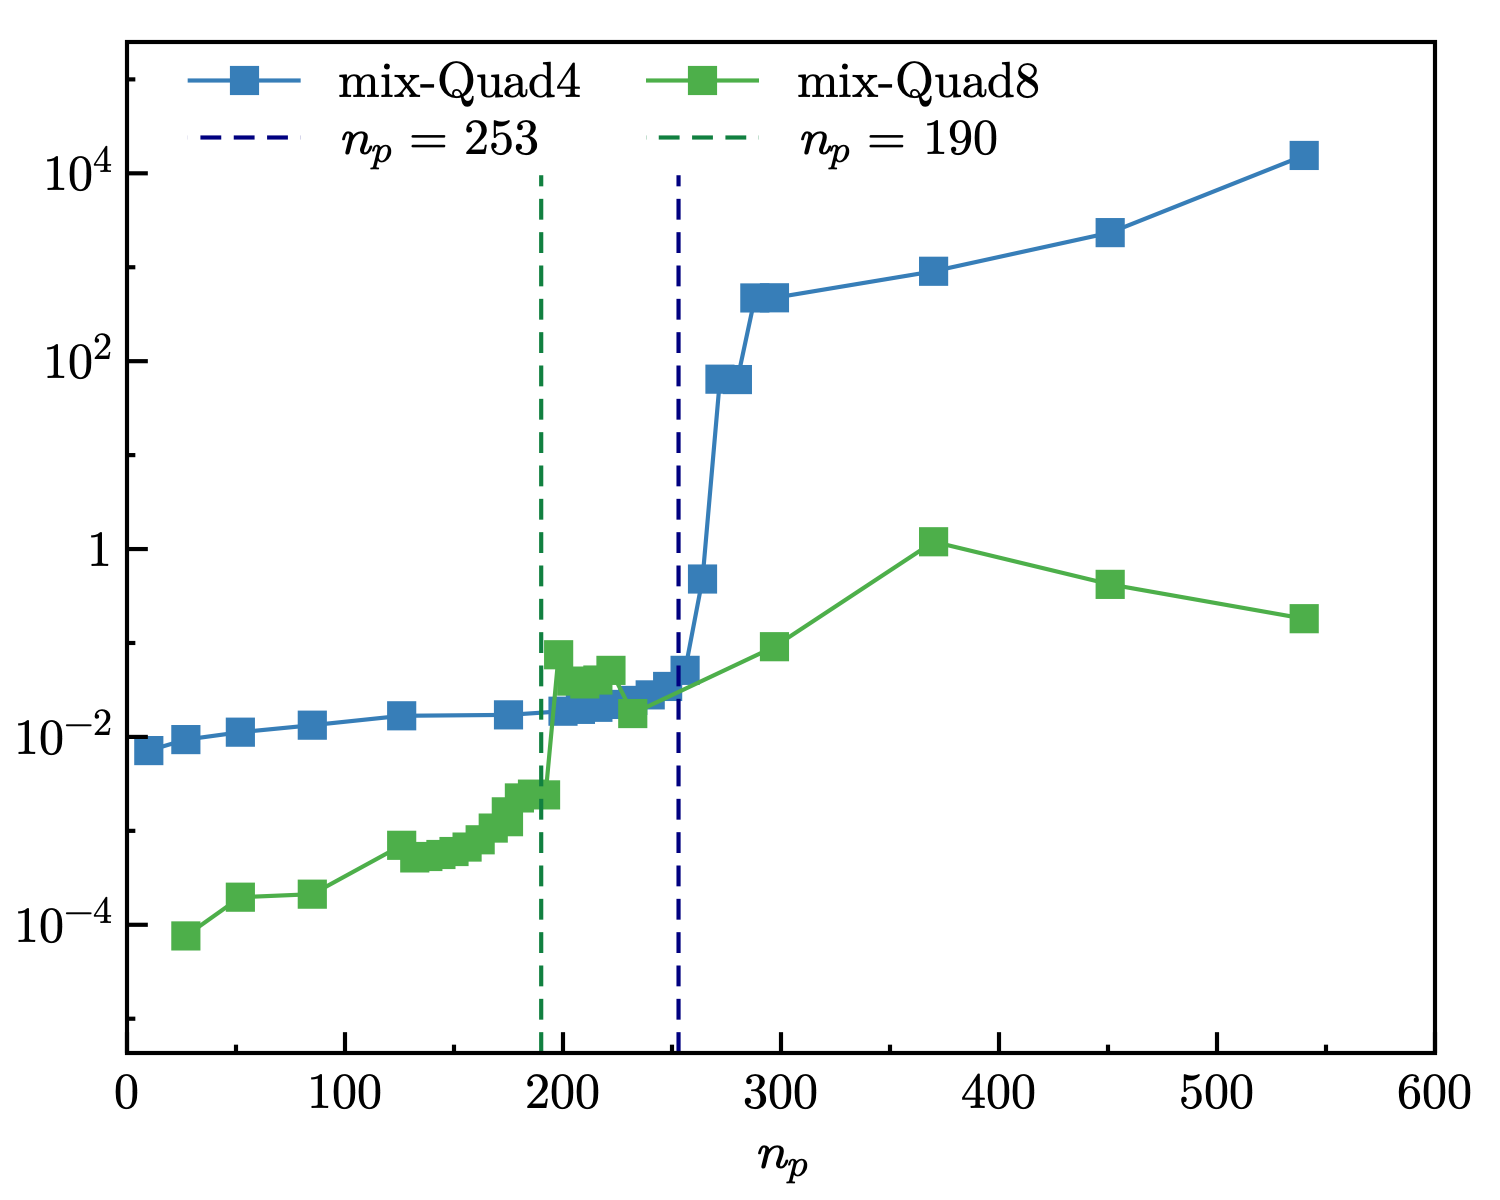
\includegraphics[width=0.45\textwidth]{figures/ch_4/cantilever_L2_p_8.png}}
        & \rotatebox{-90}{\parbox[b]{4cm}{Quad4: 297 nodes \\ Quad8: 288 nodes}} \\
          \raisebox{-0.85\height}{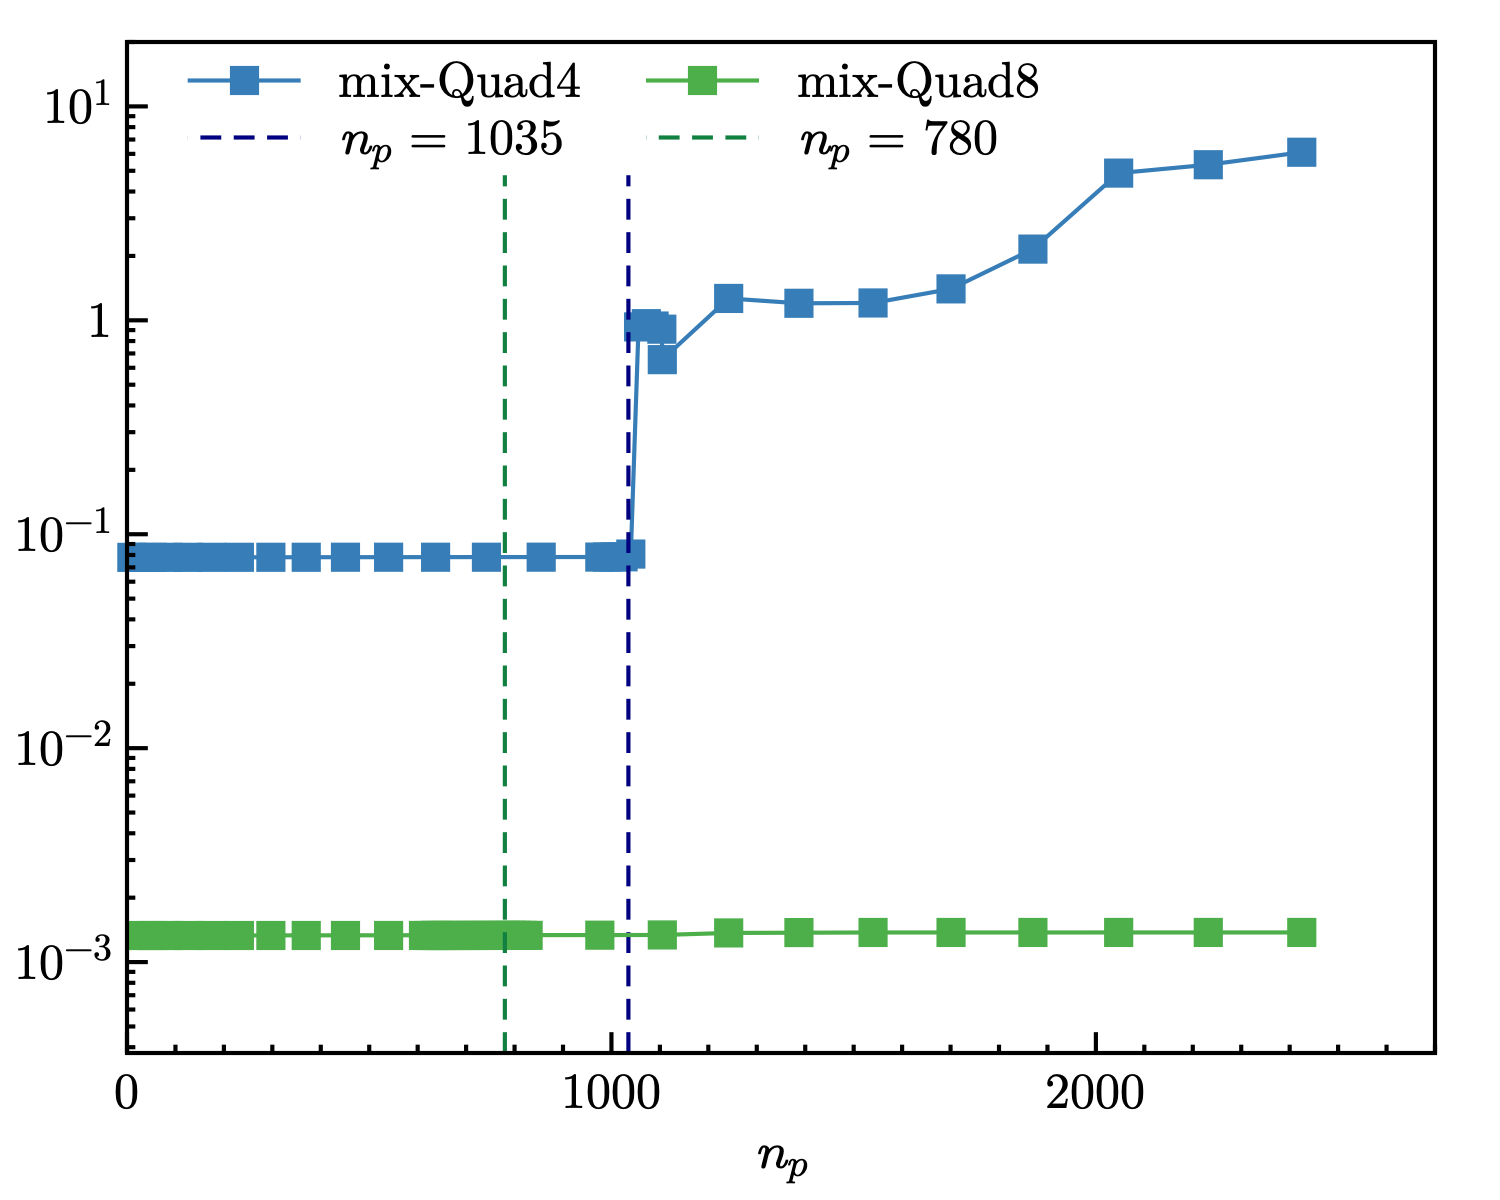
\includegraphics[width=0.45\textwidth]{figures/ch_4/cantilever_Hdev_16.png}}
        & \raisebox{-0.85\height}{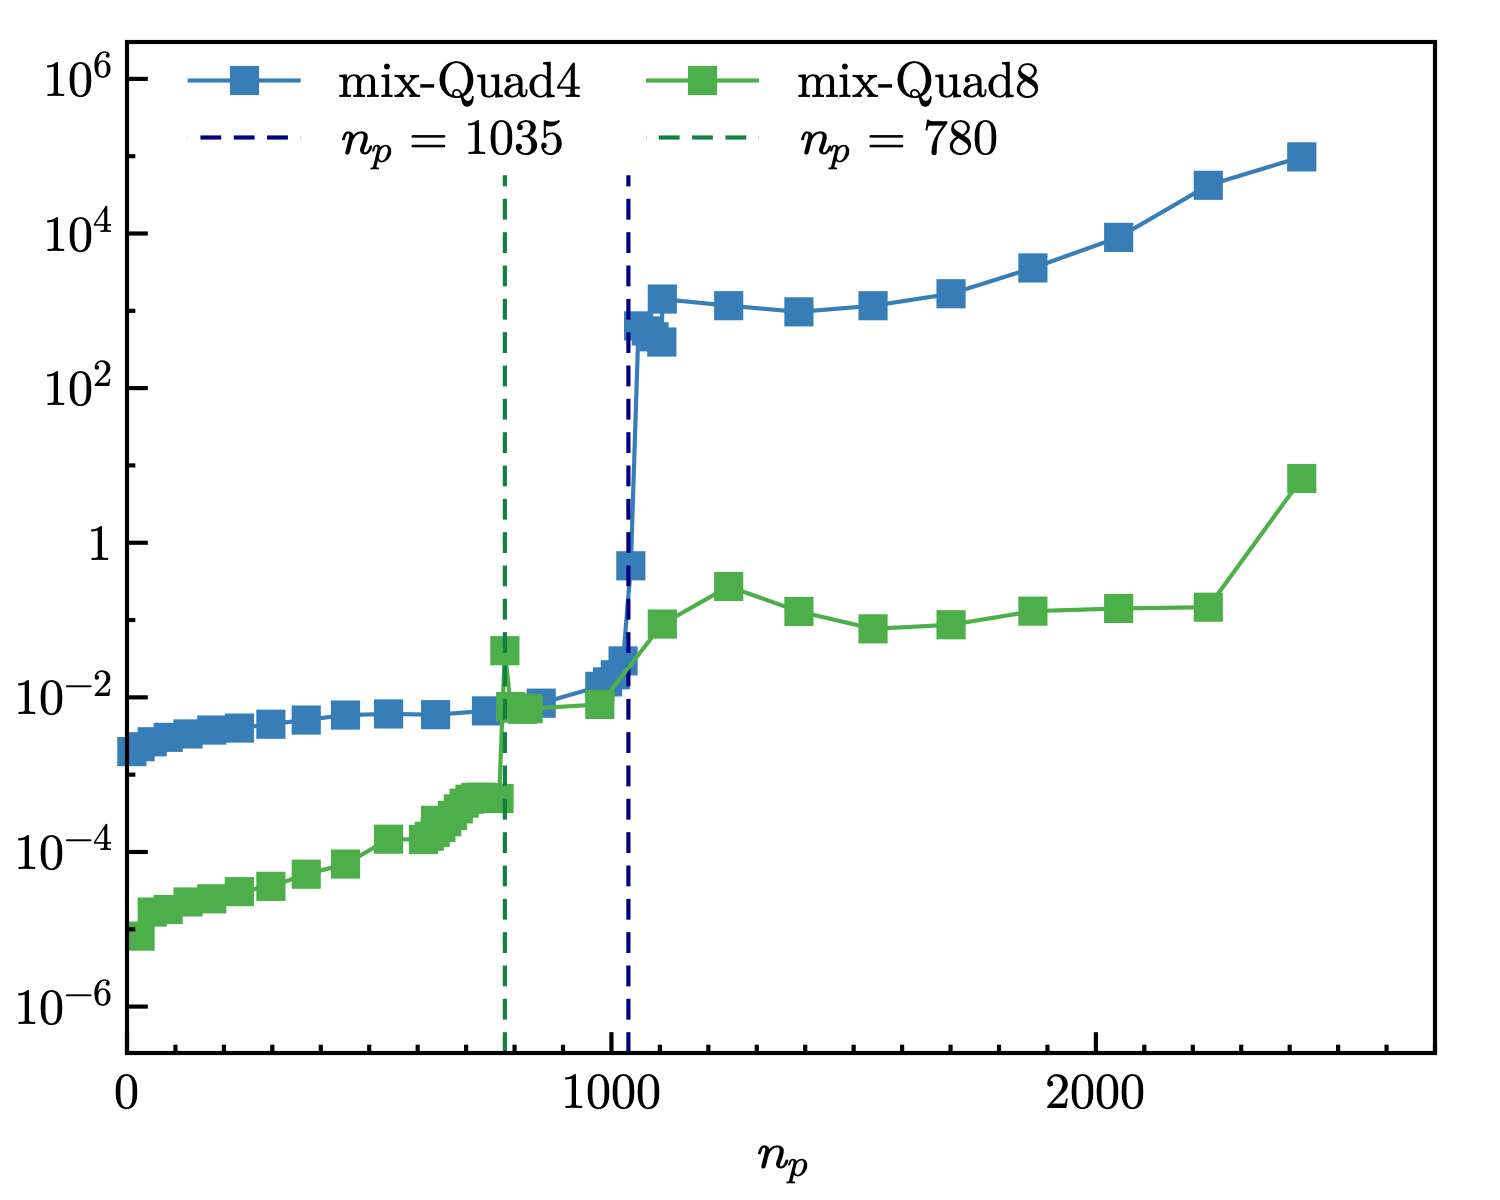
\includegraphics[width=0.45\textwidth]{figures/ch_4/cantilever_L2_p_16.png}}
        & \rotatebox{-90}{\parbox[b]{4cm}{Quad4: 1105 nodes \\ Quad8: 1088 nodes}} \\
          \raisebox{-0.85\height}{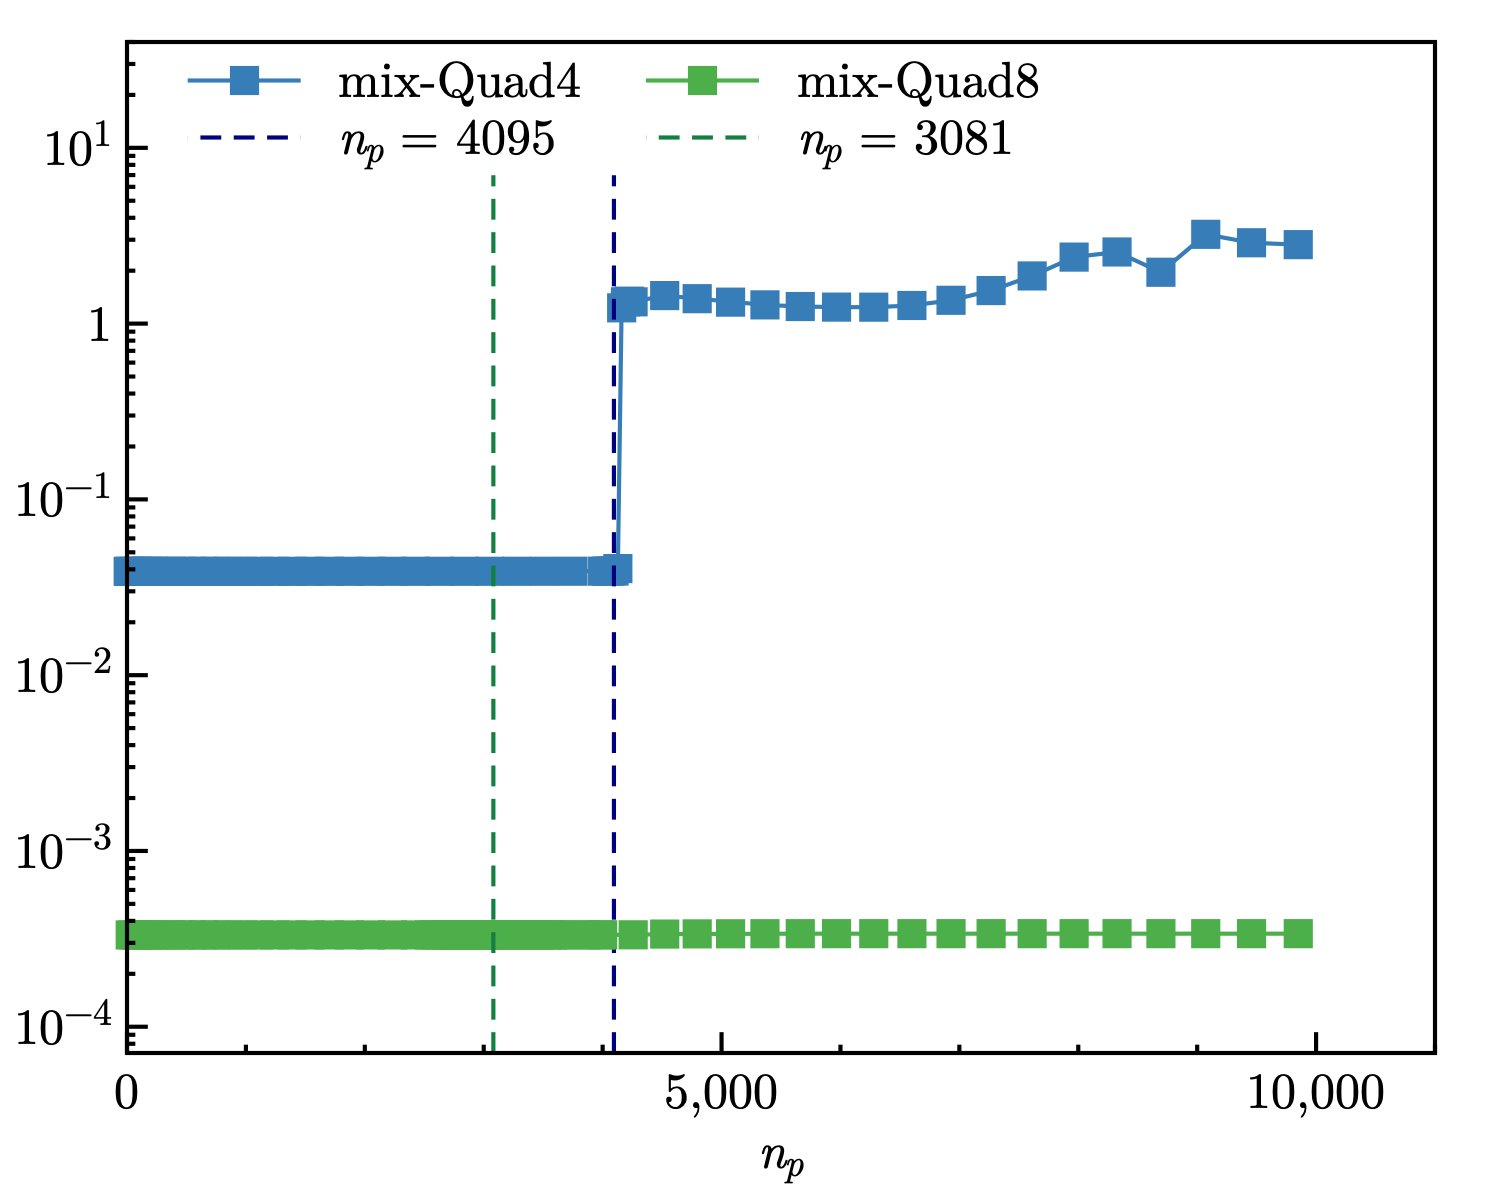
\includegraphics[width=0.45\textwidth]{figures/ch_4/cantilever_Hdev_32.png}}
        & \raisebox{-0.85\height}{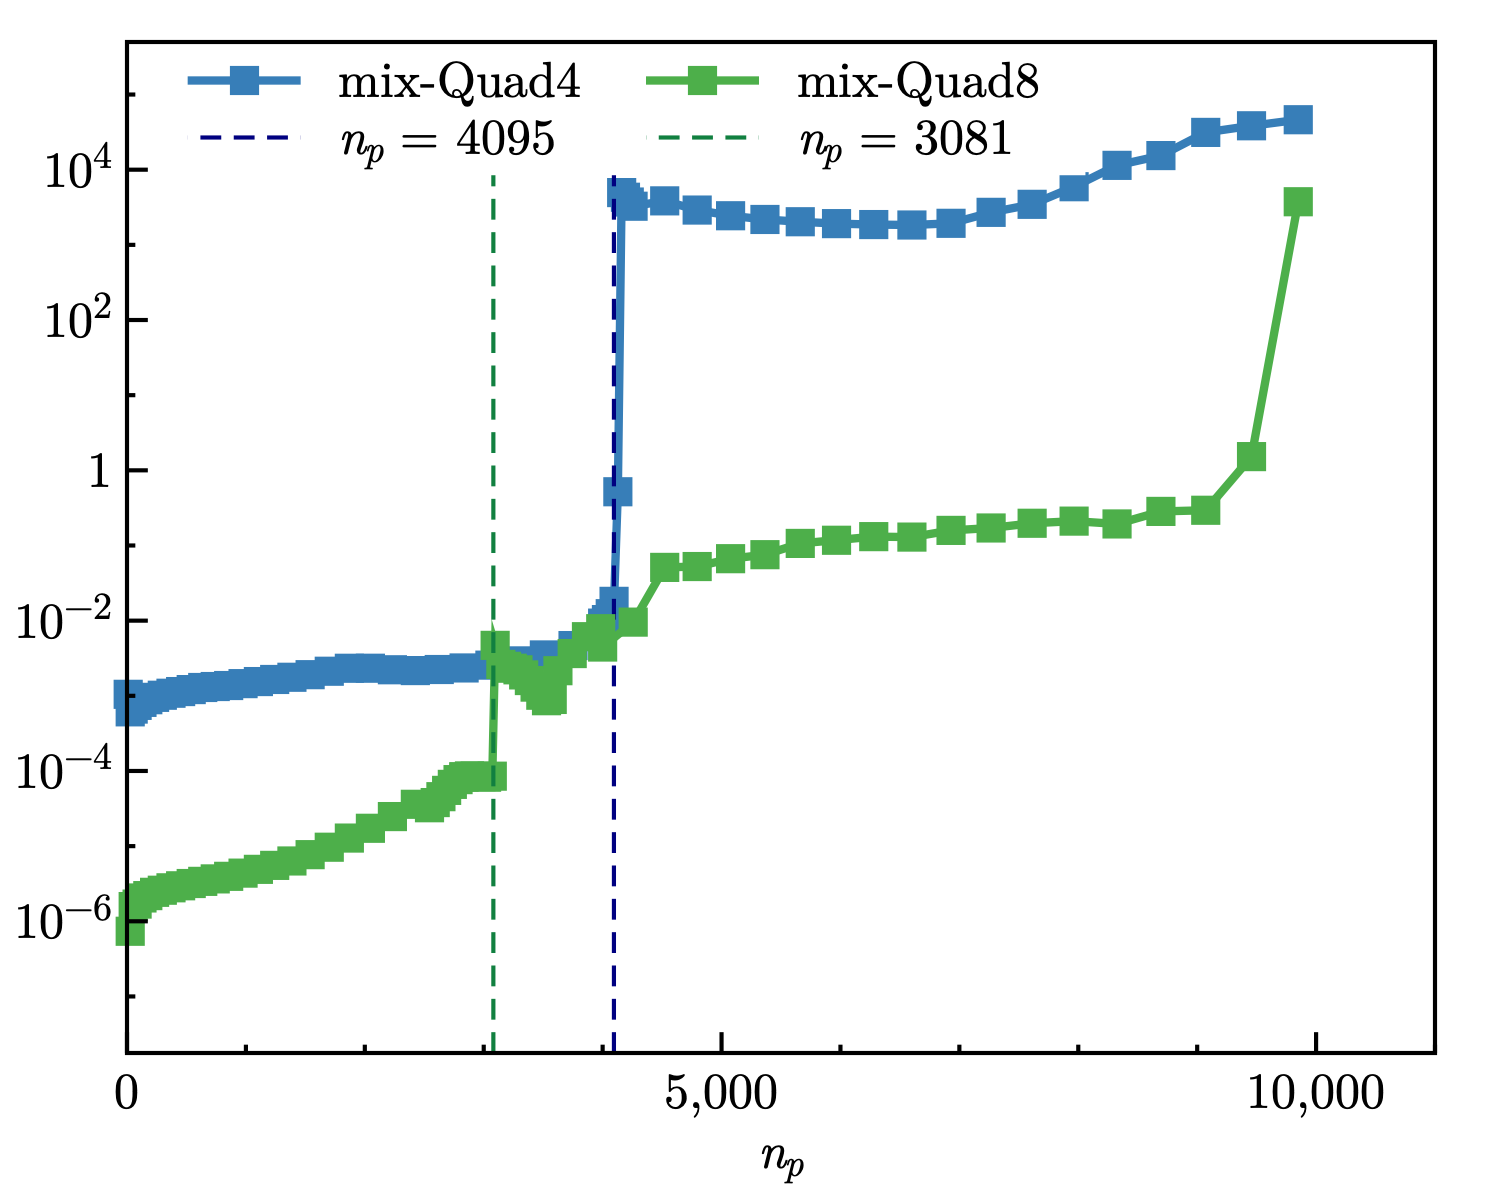
\includegraphics[width=0.45\textwidth]{figures/ch_4/cantilever_L2_p_32.png}}
        & \rotatebox{-90}{\parbox[b]{4cm}{Quad4: 4257 nodes \\ Quad8: 4224 nodes}} \\
        \end{tabular}
    \end{subcaptiongroup}
    \caption{悬臂梁问题误差与压力节点数的关系}\label{ch_4:fig:cantilever_2}
\end{figure}

\begin{figure}[H]
    \centering
    \begin{subcaptiongroup}
        \begin{tabular}{c@{\hspace{0pt}}c}
          \raisebox{-0.8\height}{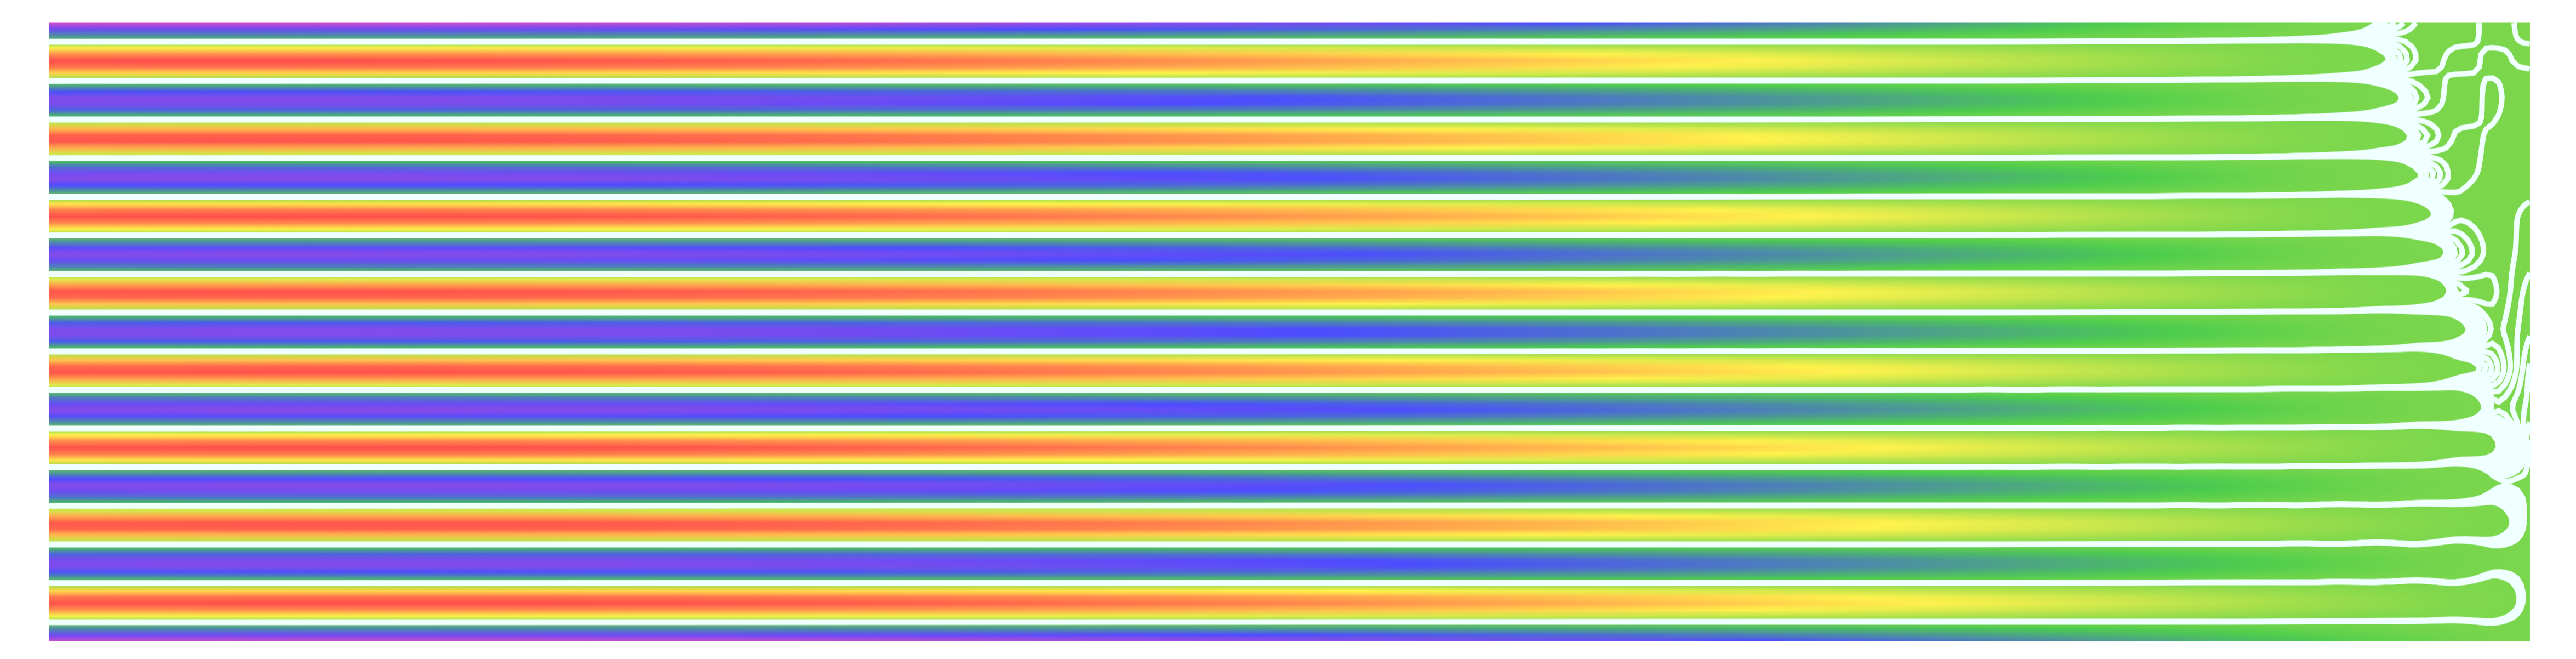
\includegraphics[width=0.8\textwidth]{figures/ch_4/cantilever_mix_quad_16_1105.png}}
        &  \\
        (a)Quad4单元$n_u=n_p=1105$(r=2)& \\
        \raisebox{-0.8\height}{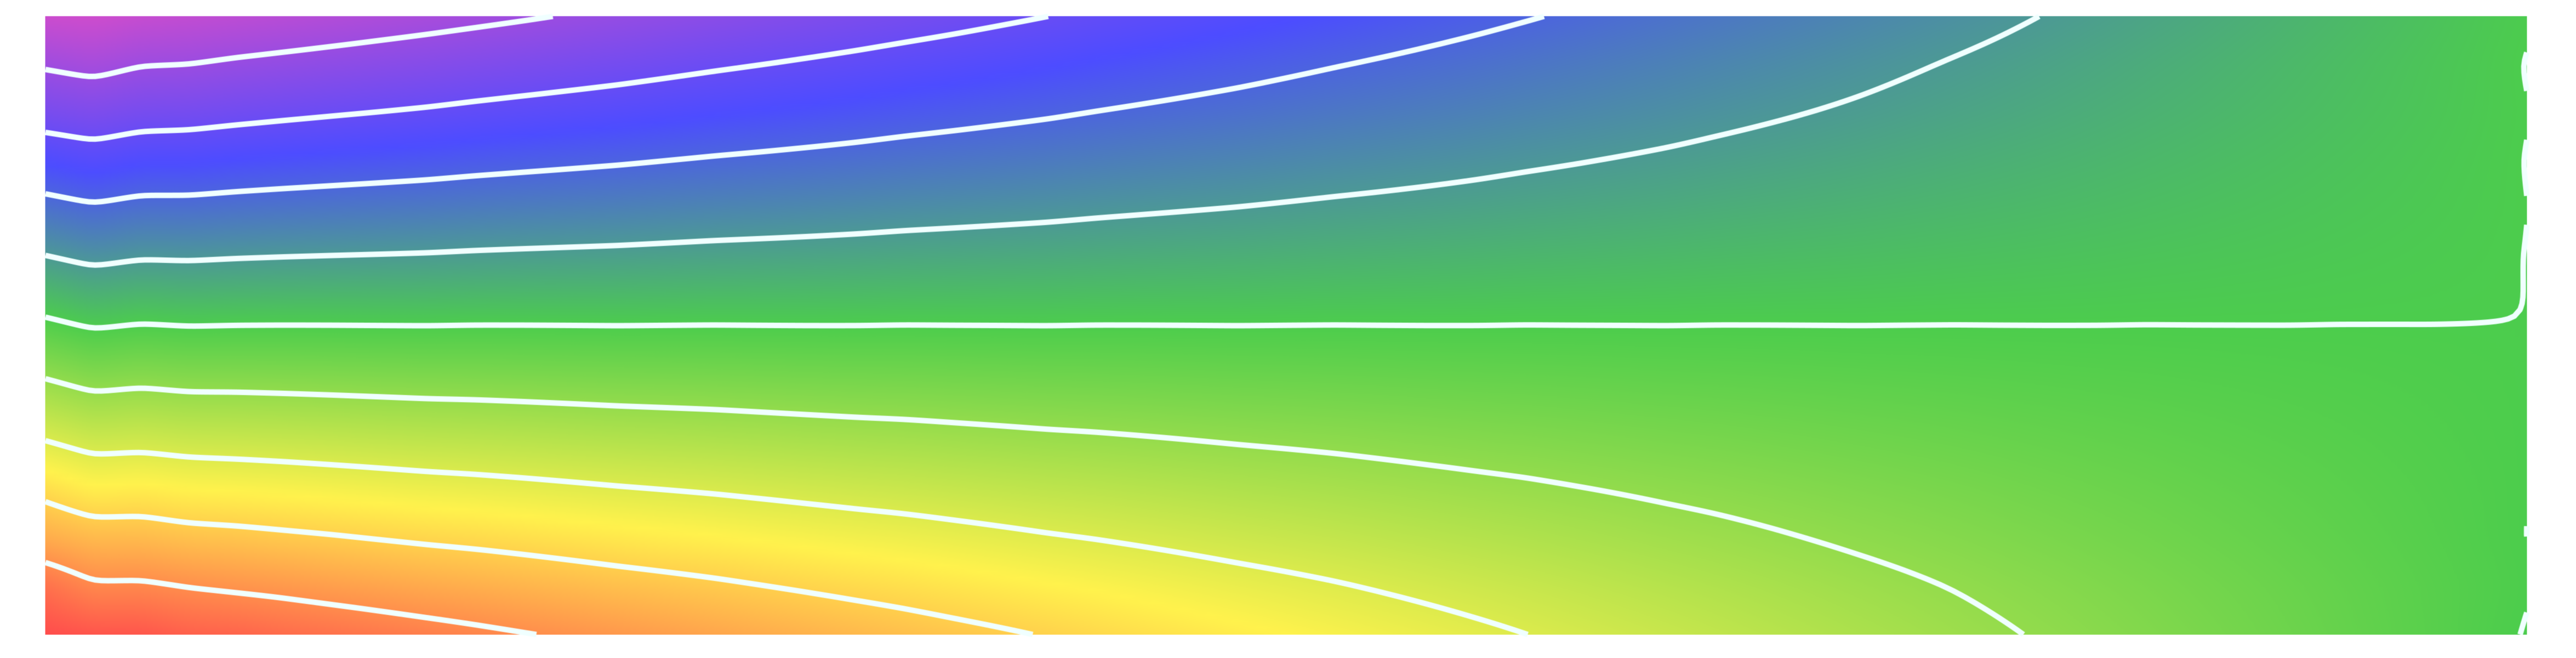
\includegraphics[width=0.8\textwidth]{figures/ch_4/cantilever_mix_quad_16_742.png}}
        &  \\
        (b)Quad4单元$n_u=1105$\,$np=742$& \\
        \raisebox{-0.8\height}{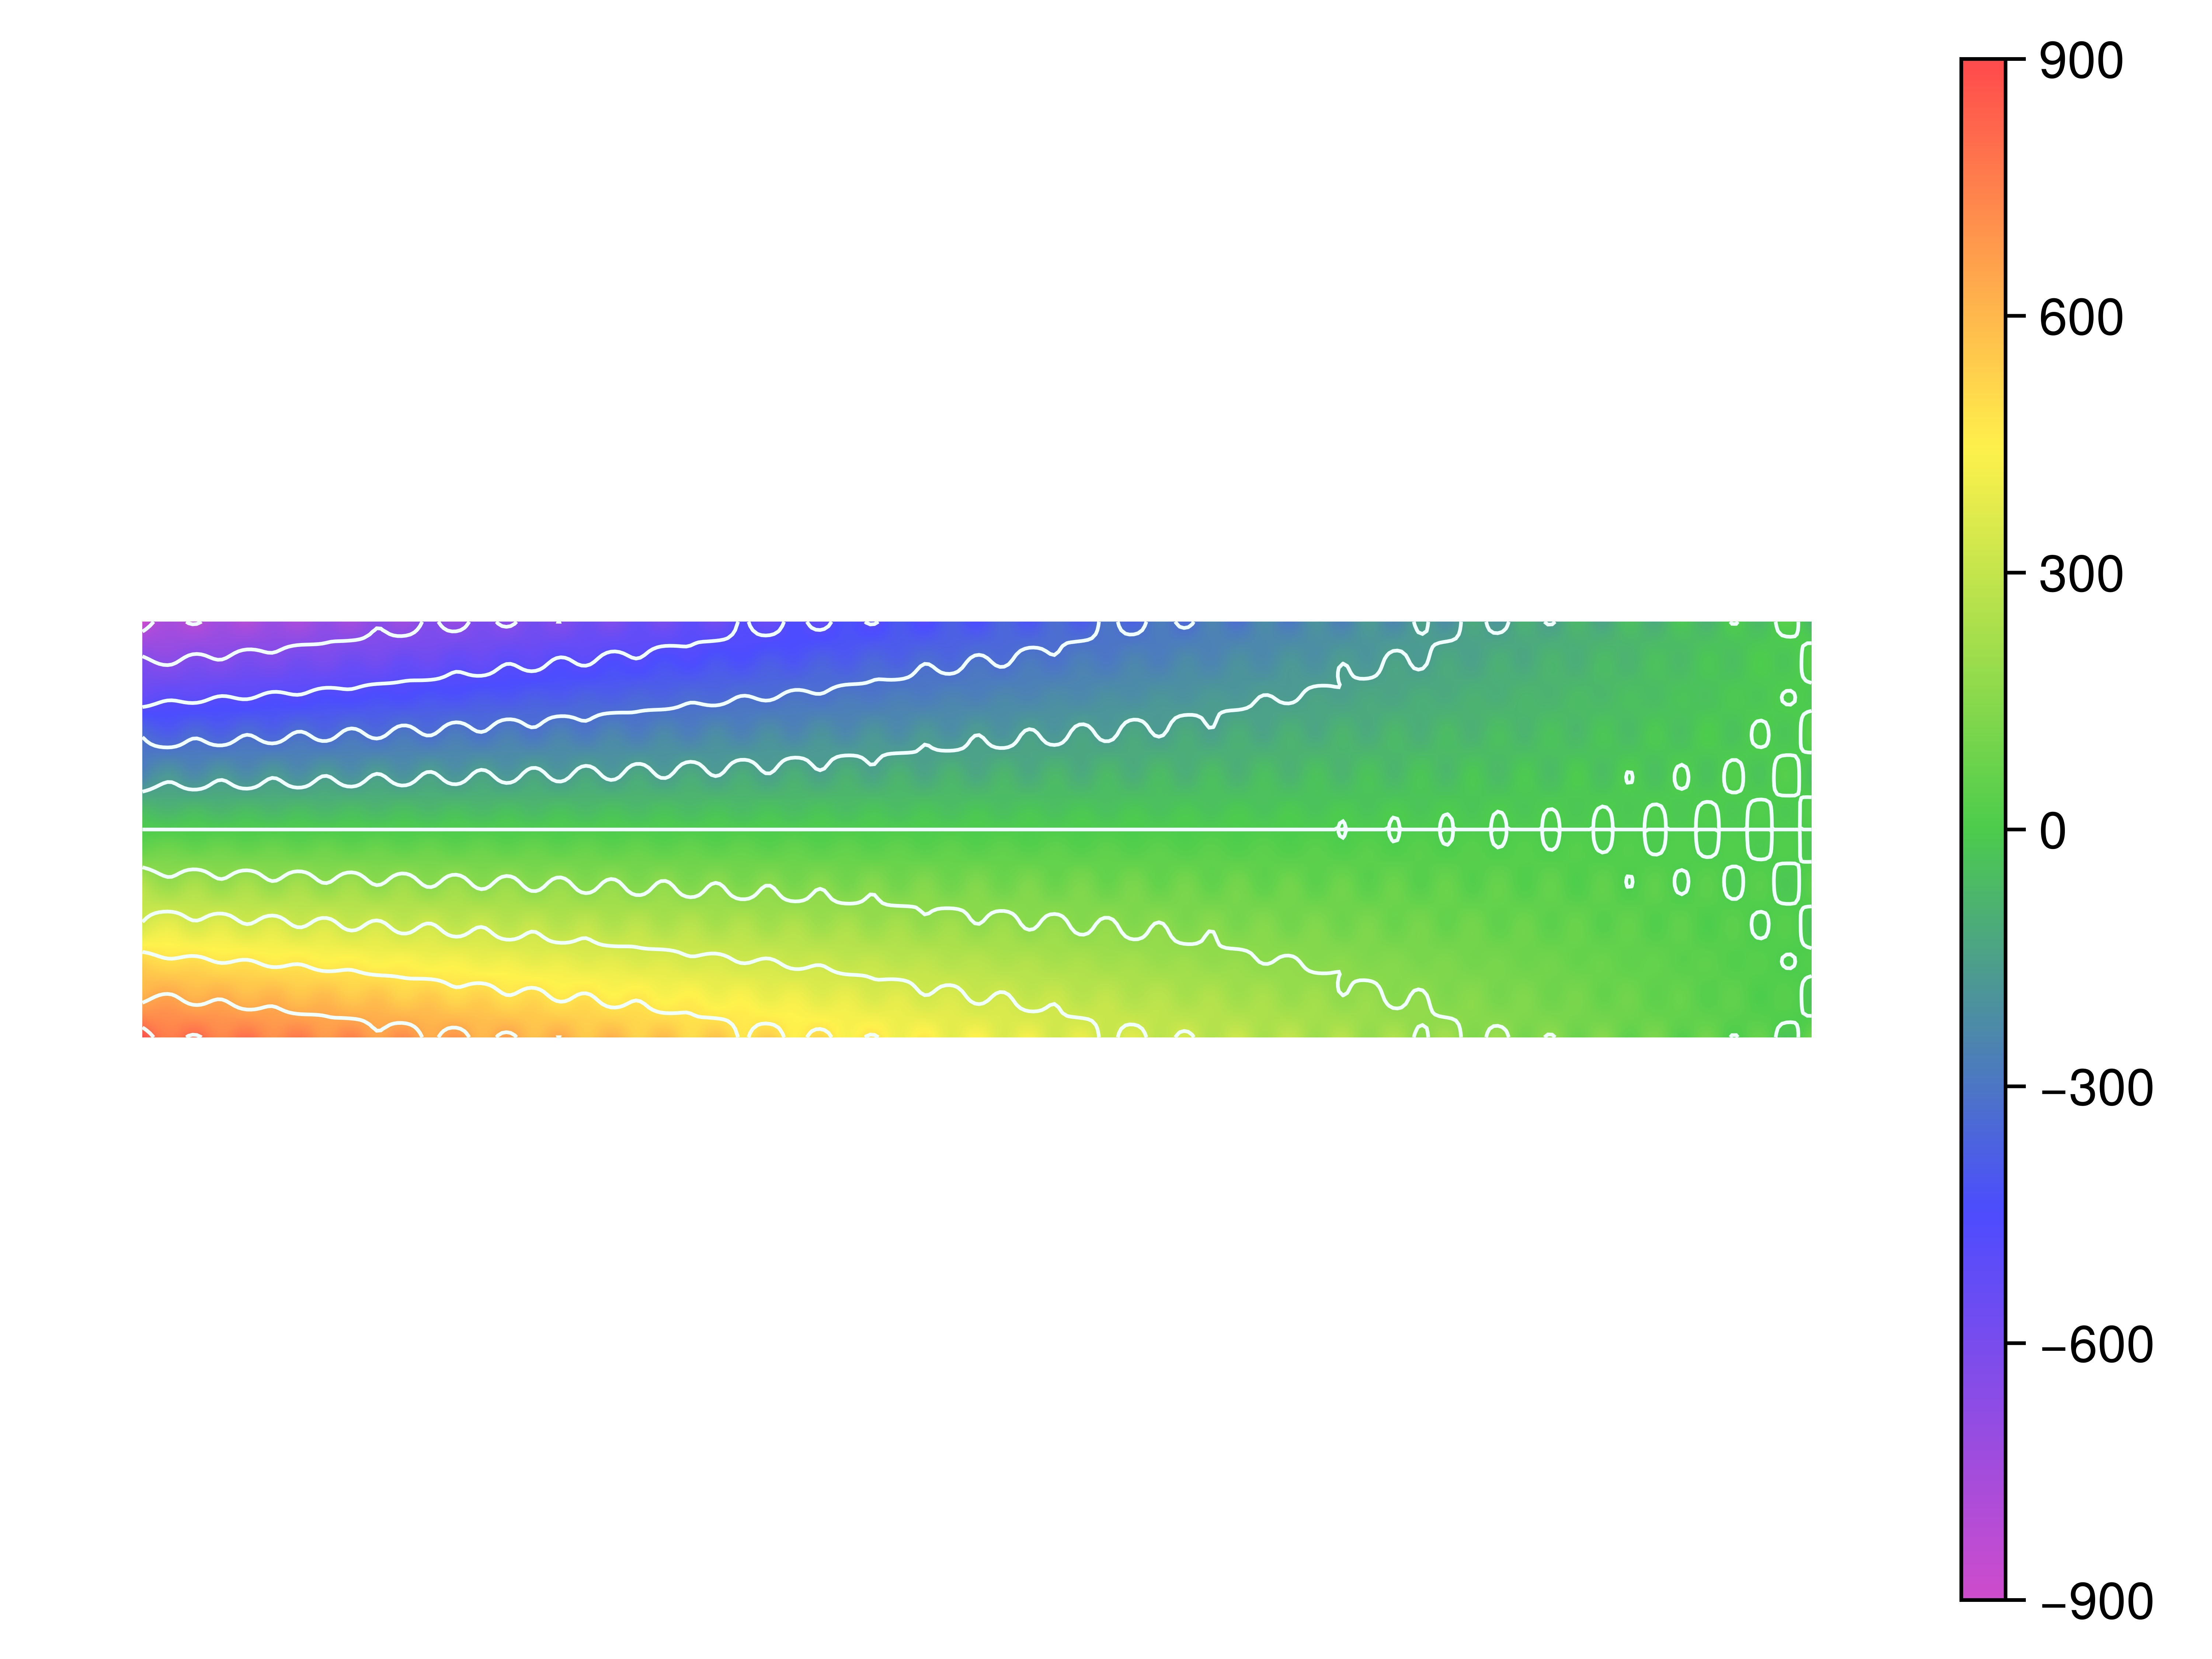
\includegraphics[width=0.8\textwidth]{figures/ch_4/cantilever_mix_quad8_8_780.png}}
        & \multirow{4}{*}{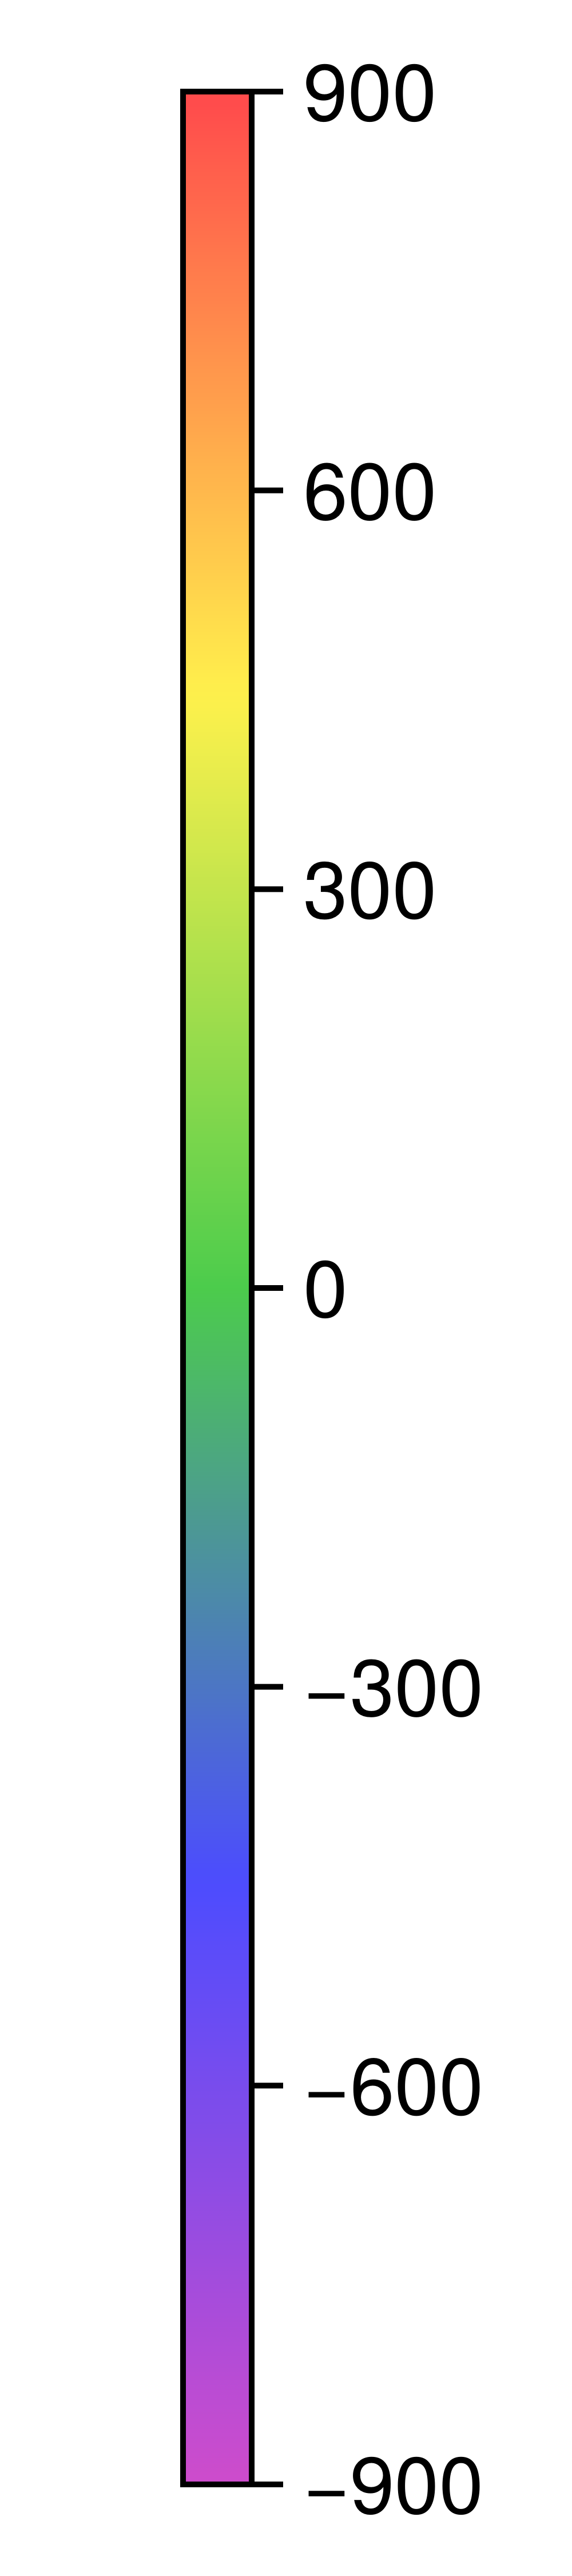
\includegraphics[width=0.1\textwidth]{figures/ch_4/cantilever_mix_colorbar.png}} \\
        (c)Quad8单元$n_u=1088$\,$n_p=780$& \\
        \raisebox{-0.8\height}{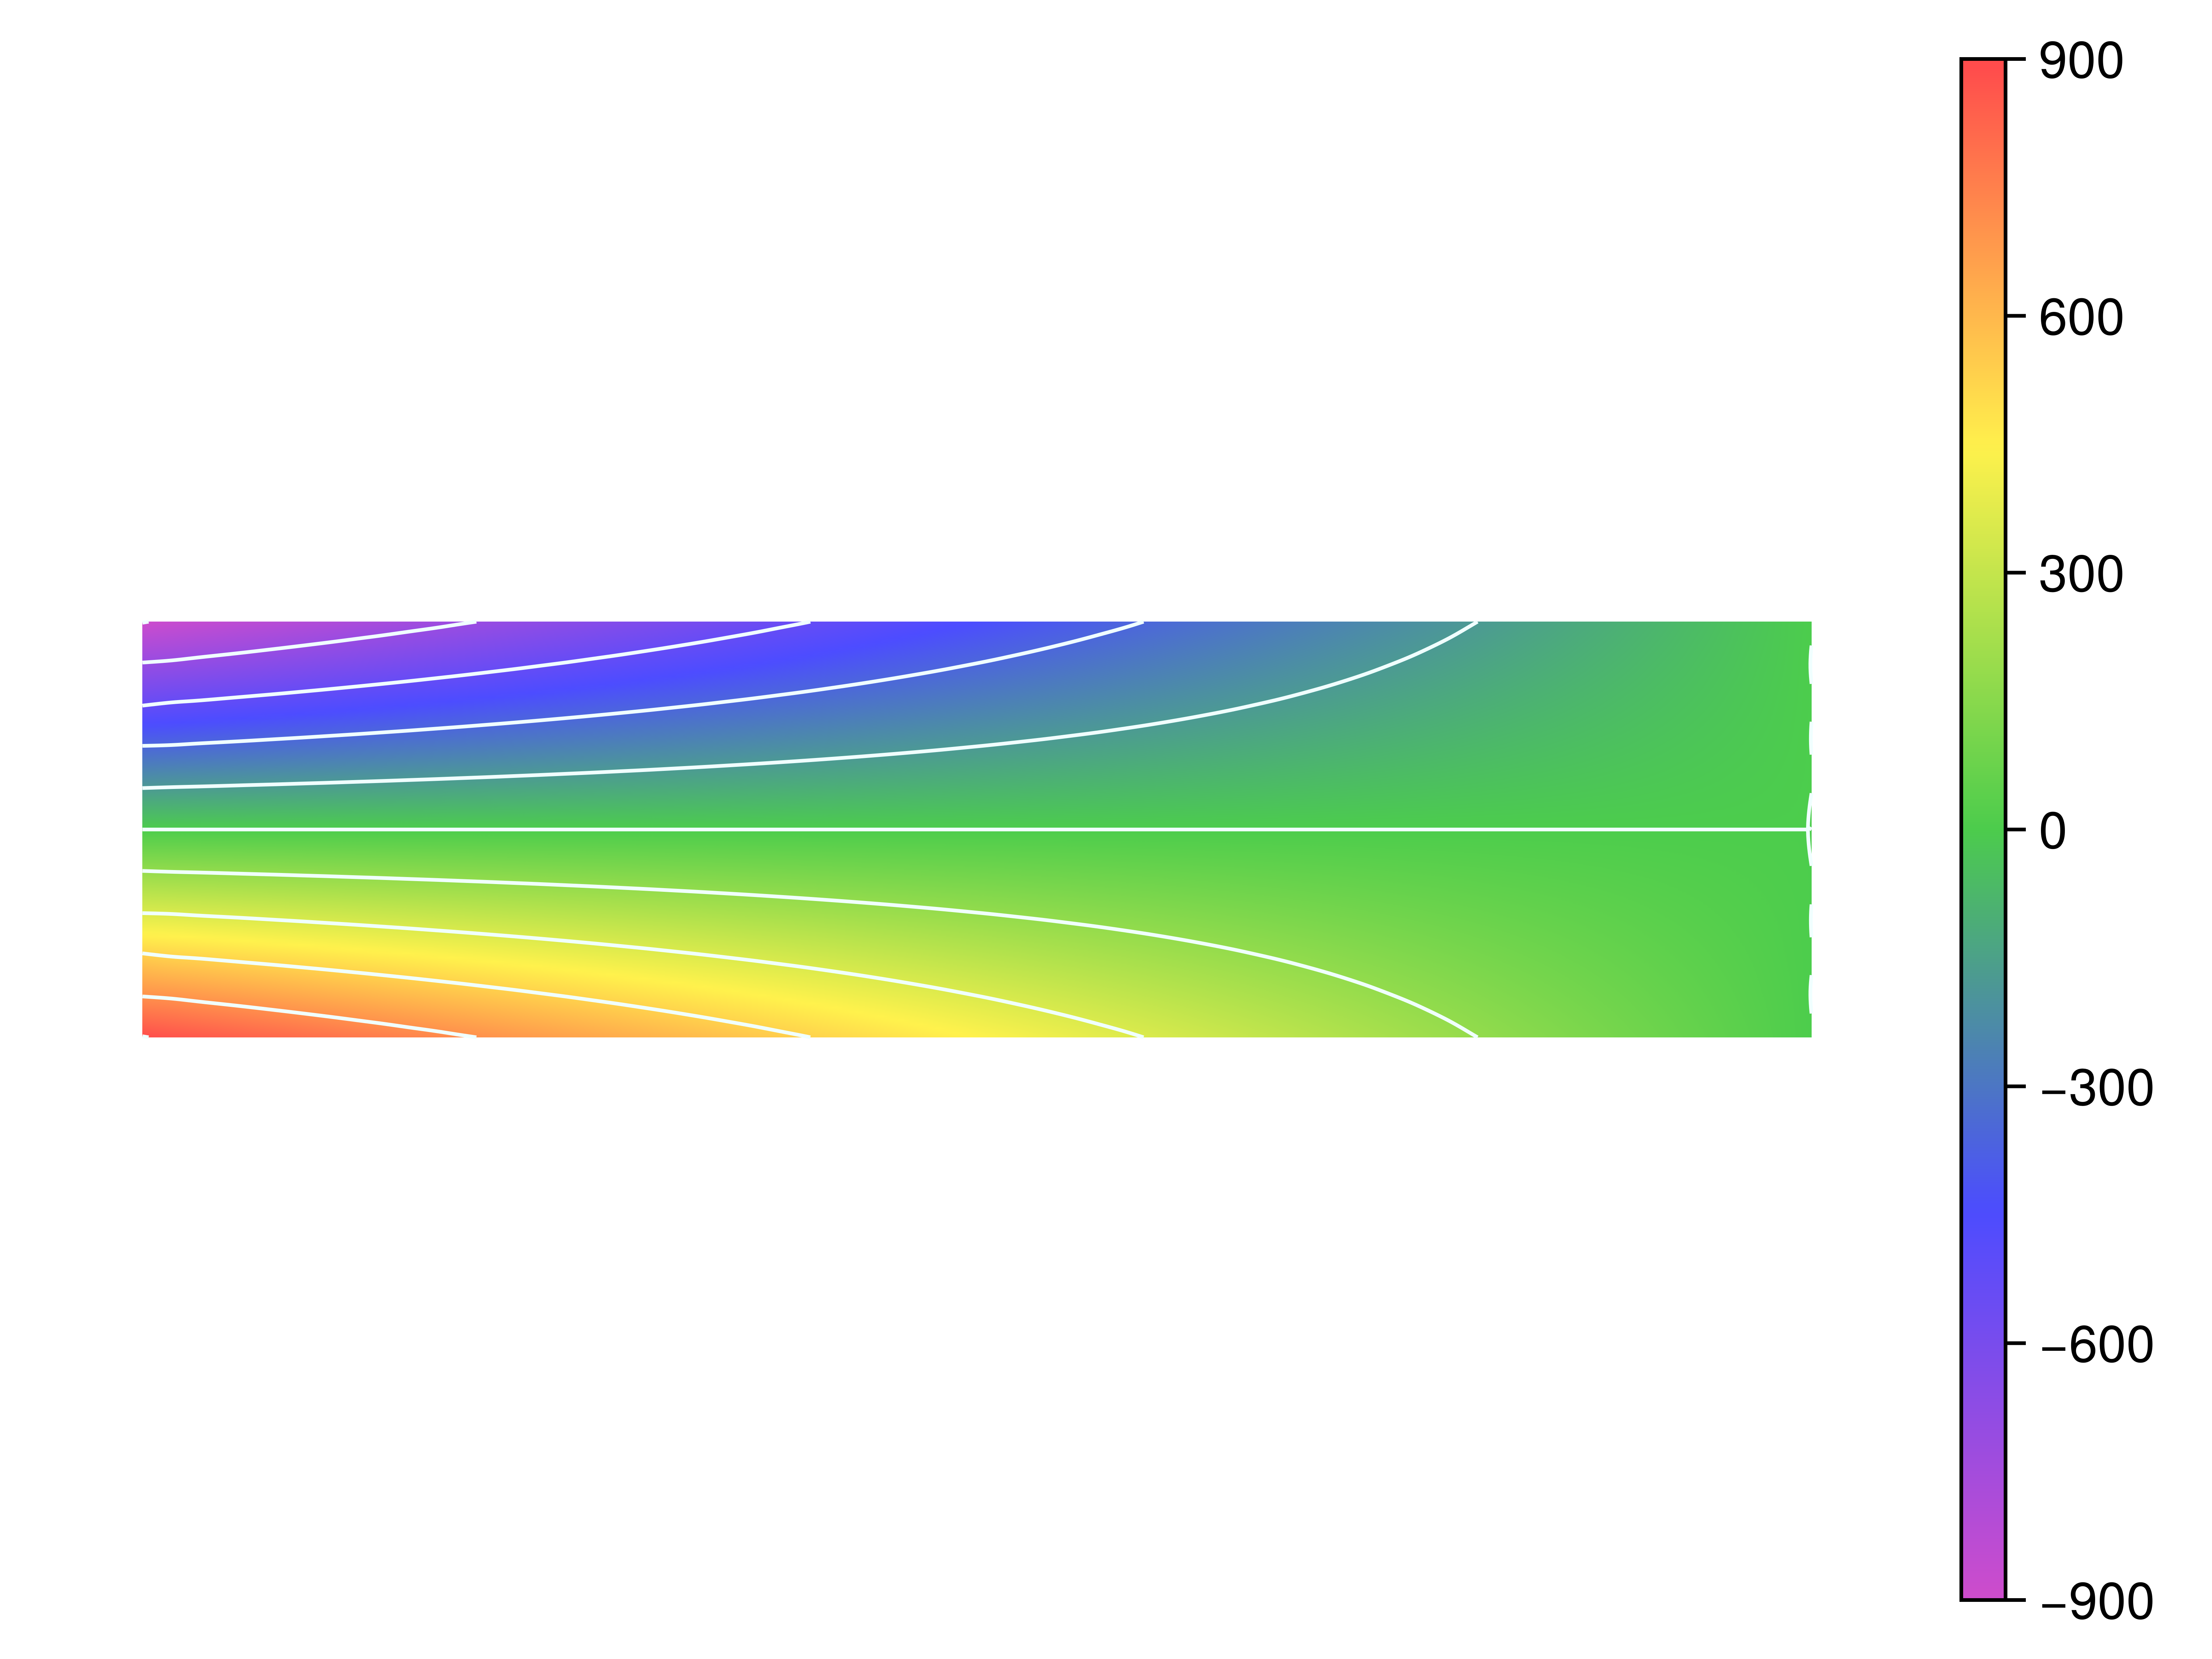
\includegraphics[width=0.8\textwidth]{figures/ch_4/cantilever_mix_quad8_8_768.png}}
        &  \\
        (d)Quad8单元$n_u=1088$\,$np=768$& \\
        \end{tabular}
    \end{subcaptiongroup}
    \caption{悬臂梁问题压力云图}\label{ch_4:fig:cantilever_P}
\end{figure}

\begin{figure}[H]
    \centering
    \begin{subcaptiongroup}
        \begin{tabular}{c@{\hspace{0pt}}c}
          \raisebox{-0.8\height}{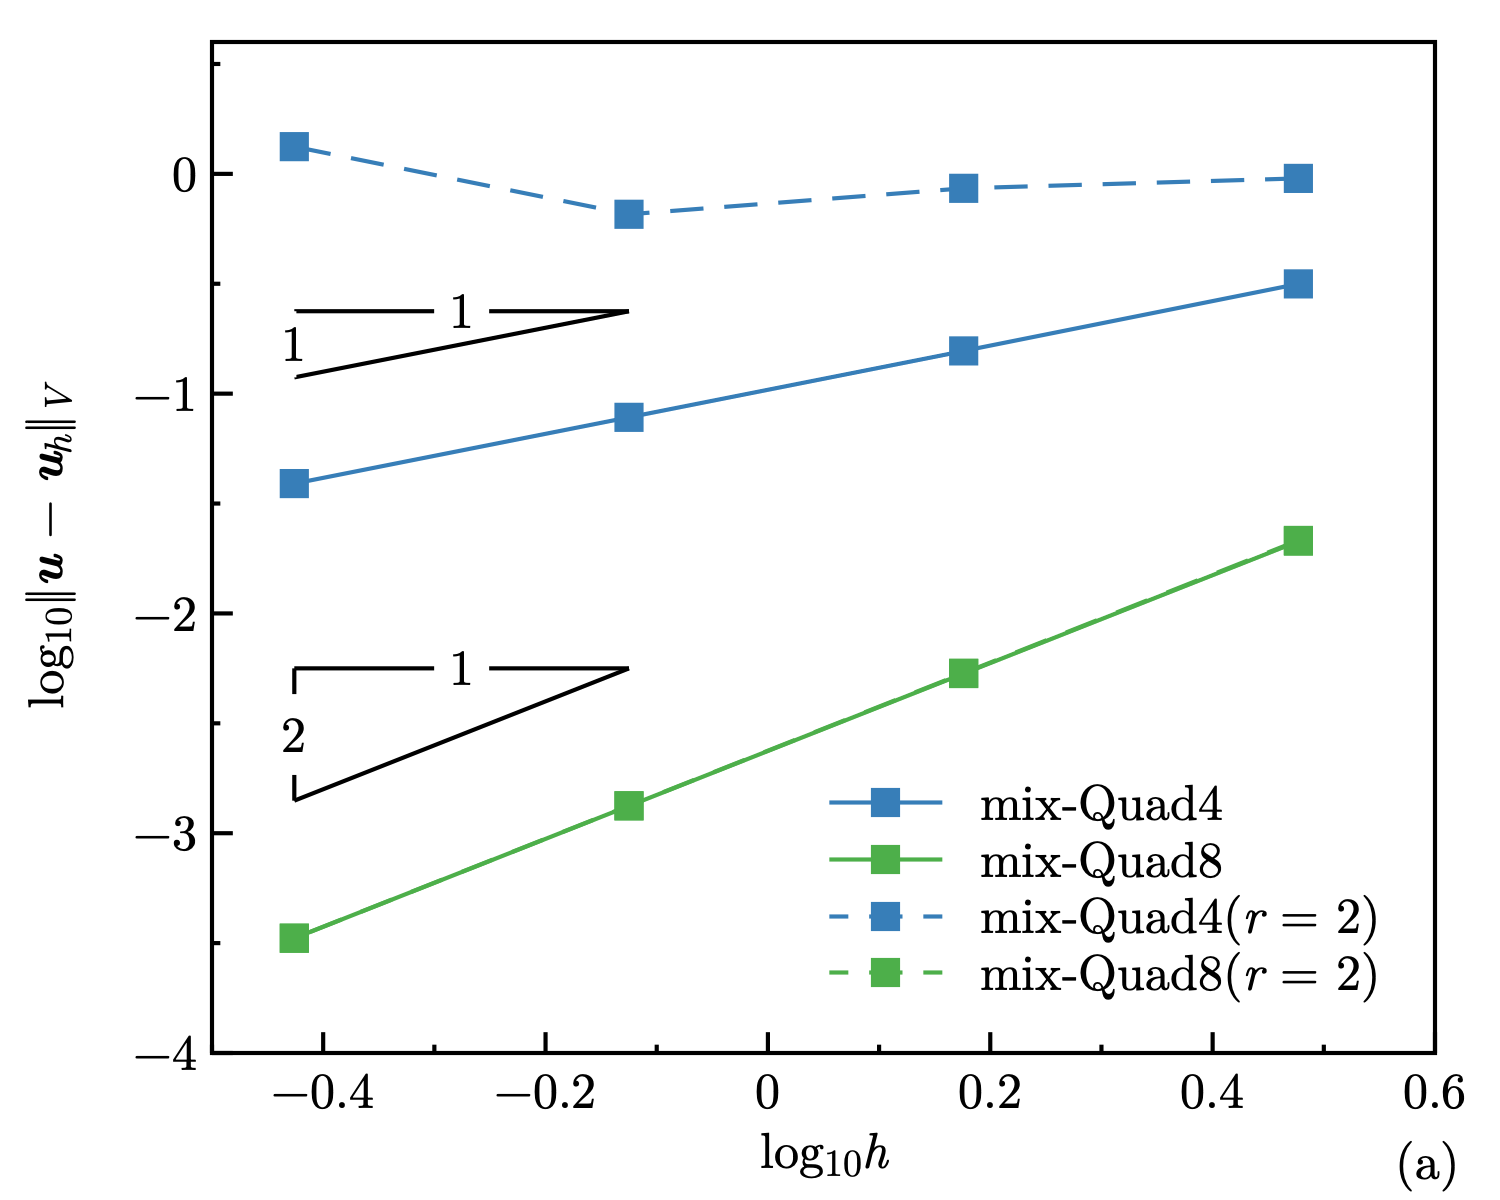
\includegraphics[width=0.5\textwidth]{figures/ch_4/cantilever_Hdev.png}}
        & \raisebox{-0.8\height}{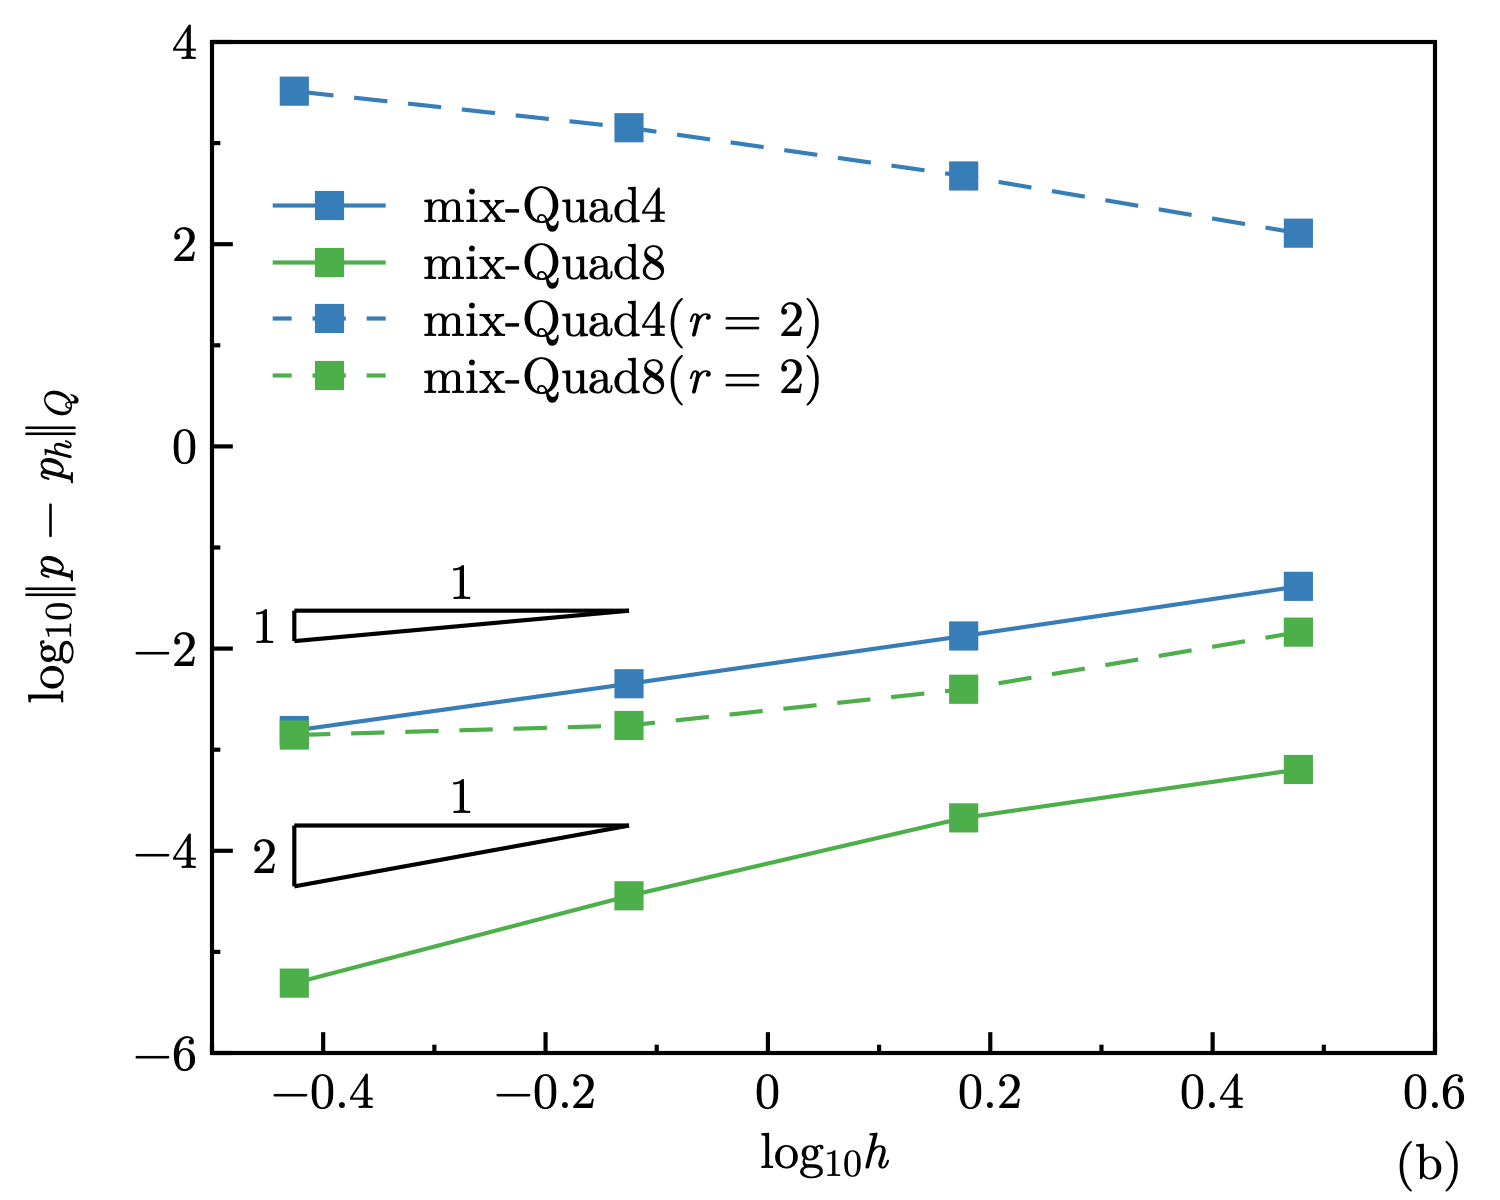
\includegraphics[width=0.5\textwidth]{figures/ch_4/cantilever_L2_p.png}}\\
        \end{tabular}
    \end{subcaptiongroup}
    \caption{悬臂梁问题误差对比}\label{ch_4:fig:cantileve_l2}
\end{figure}
\subsection{带孔无限大平板问题}

考虑经典的带孔无限大平板问题,如图\ref{ch_4:fig:hole}所示,板的的中心存在一半径为$a=1$的圆形小孔,同时平板的无穷远处沿$x$轴方向施加均布荷载$T=1000$。 板的材料系数为杨氏模量$E=3\times10^6$、泊松比$\nu=0.49999$。根据Michell解可以得到该带孔无限大平板问题的解析解为:
\begin{equation}\label{ch_4:eq:plate_with_hole_exact}
    \begin{split}
        u_x(r,\theta)&=\frac{Ta}{8\mu}(\frac{r}{a}(k+1)\cos\theta-\frac{2a^3}{r^3}\cos3\theta    +\frac{2a}{r}((1+k)\cos\theta+\cos3\theta))\\
        u_y(r,\theta)&=\frac{Ta}{8\mu}(\frac{r}{a}(k-3)\sin\theta-\frac{2a^3}{r^3}\sin3\theta    +\frac{2a}{r}((1-k)\sin\theta+\sin3\theta))  
    \end{split}
\end{equation}
其中,$k$和$\mu$分别为:
\begin{equation}
    \begin{split}
        k=\frac{3-\nu}{1+\nu}\quad \text{,}\mu=\frac{E}{2(1+\nu)}
    \end{split}
\end{equation}
与之相对应的应力分量为:
\begin{equation}
\begin{split}
    \sigma_{xx}&=T(1-\frac{a^2}{r^2}(\frac{3}{2}\cos2\theta+\cos4\theta)+\frac{3a^4}{2r^4}\cos4\theta)\\
    \sigma_{yy}&=-T(\frac{a^2}{r^2}(\frac{1}{2}\cos2\theta-\cos4\theta)+\frac{3a^4}{2r^4}\cos4\theta)\\
    \sigma_{xy}&=-T(\frac{a^2}{r^2}(\frac{1}{2}\sin2\theta+\sin4\theta)-\frac{3a^4}{2r^4}\sin4\theta)\\
\end{split}
\end{equation}

\begin{figure}[!h]
    \centering 
        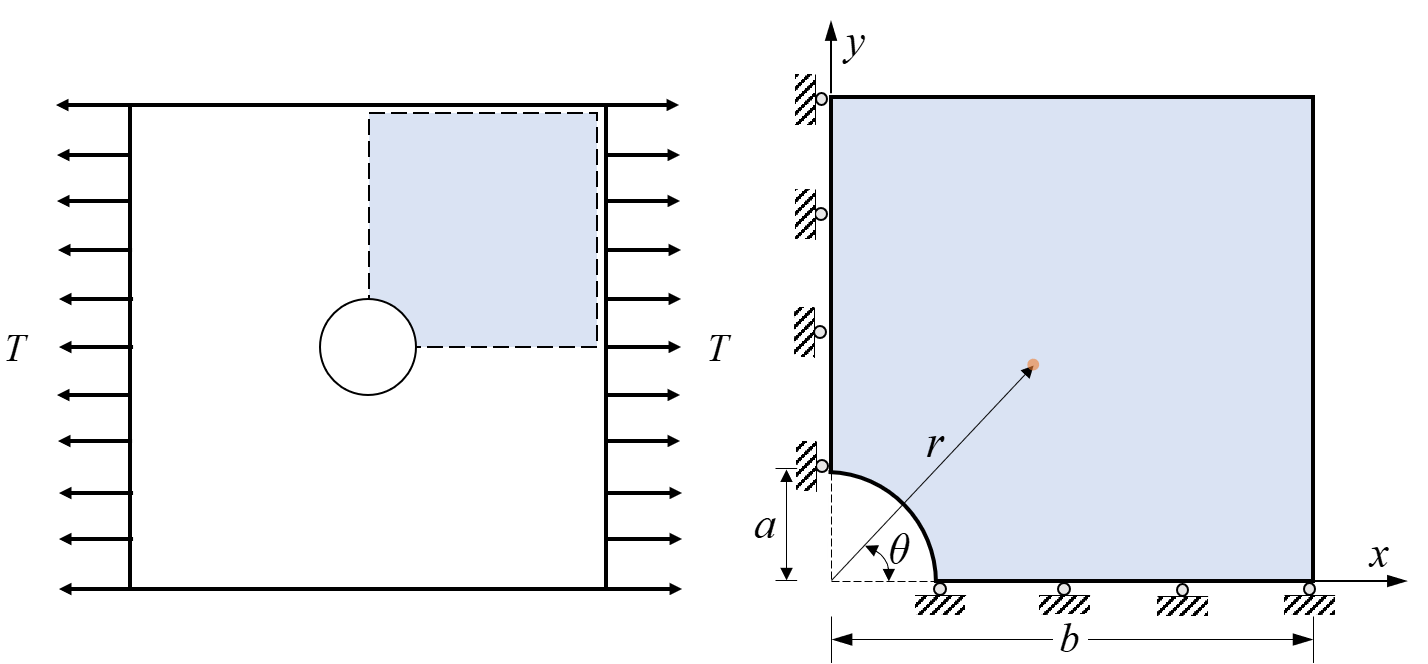
\includegraphics[scale=0.5]{figures/ch_4/hole.png}
        \caption{带孔方板问题模型}\label{ch_4:fig:hole}
\end{figure}

根据带孔无限大平板的对称性,如图\ref{ch_4:fig:hole}所示,取边长$b=5$的四分之一方形域进行研究,求解域的左端与下端约束法向位移,求解域上端和右端根据式\eqref{ch_4:eq:plate_with_hole_exact}施加自然边界条件。


\begin{figure}[H]
    \centering
    \begin{subcaptiongroup}
        \begin{tabular}{c@{\hspace{0pt}}c@{\hspace{0pt}}c}
          $\Vert \boldsymbol u - \boldsymbol u_h \Vert_V$ & $\Vert p - p_h \Vert_Q$ & $n_u$\\
          \raisebox{-0.7\height}{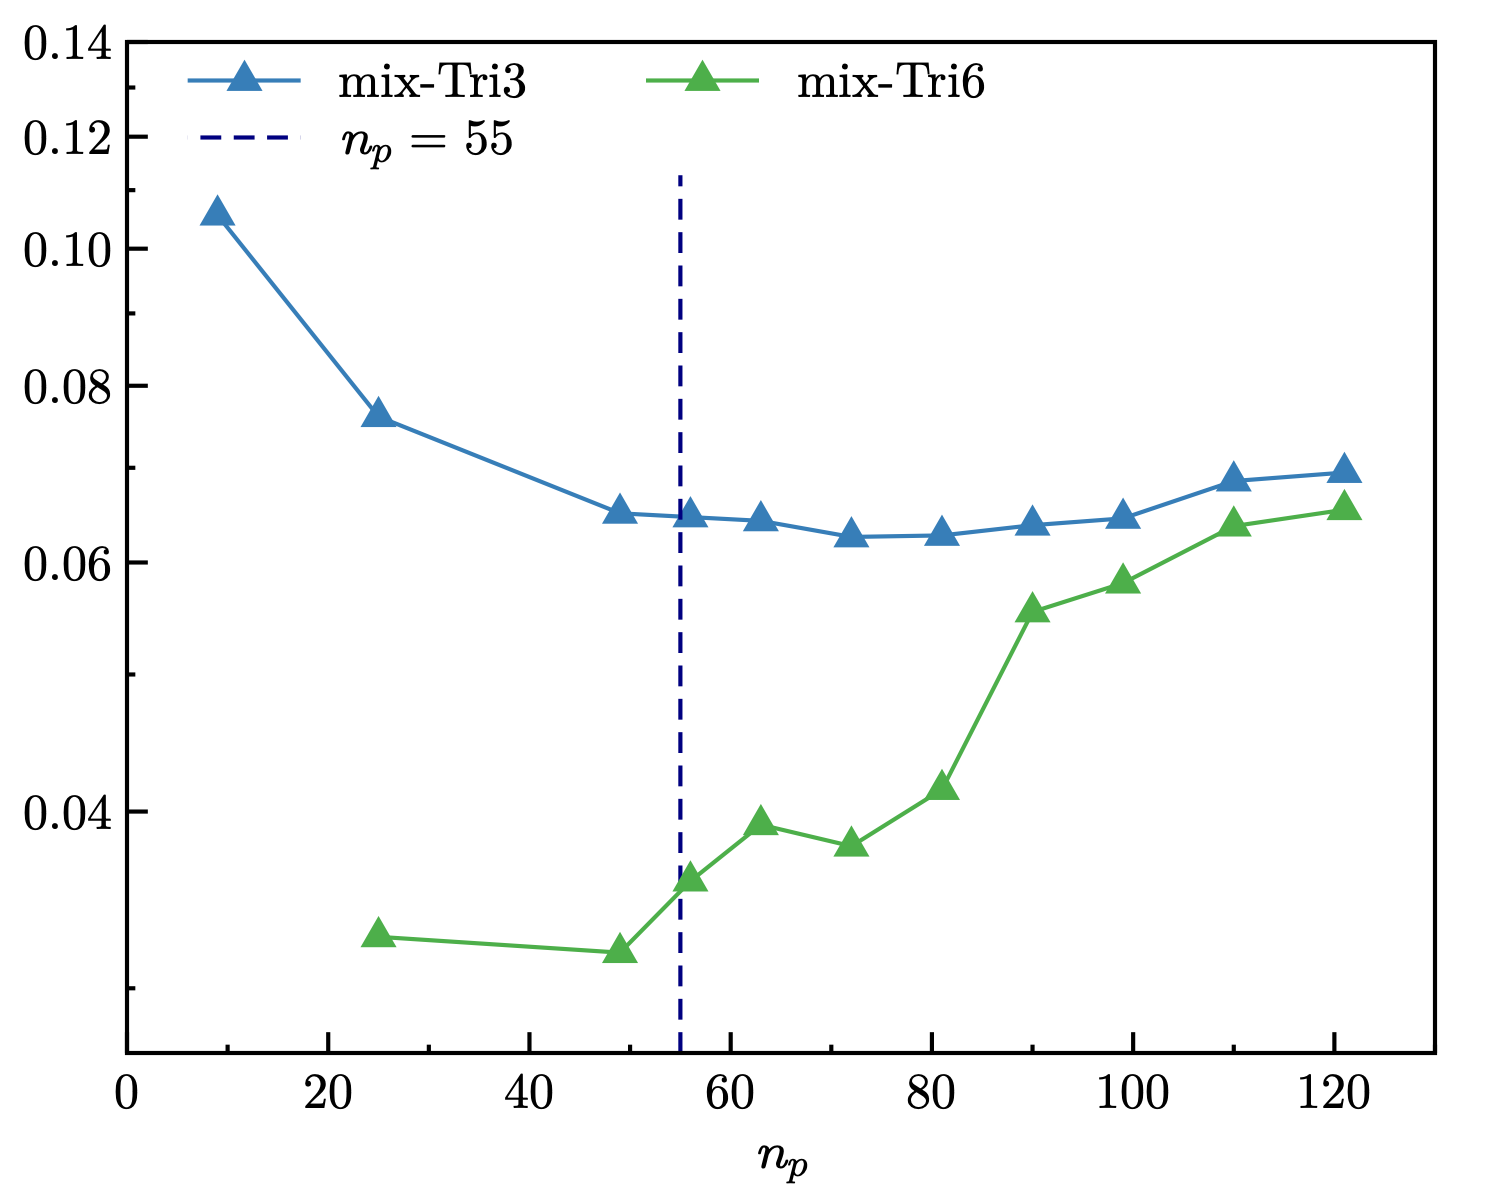
\includegraphics[width=0.45\textwidth]{figures/ch_4/plate_Hdev_4.png}}
        & \raisebox{-0.7\height}{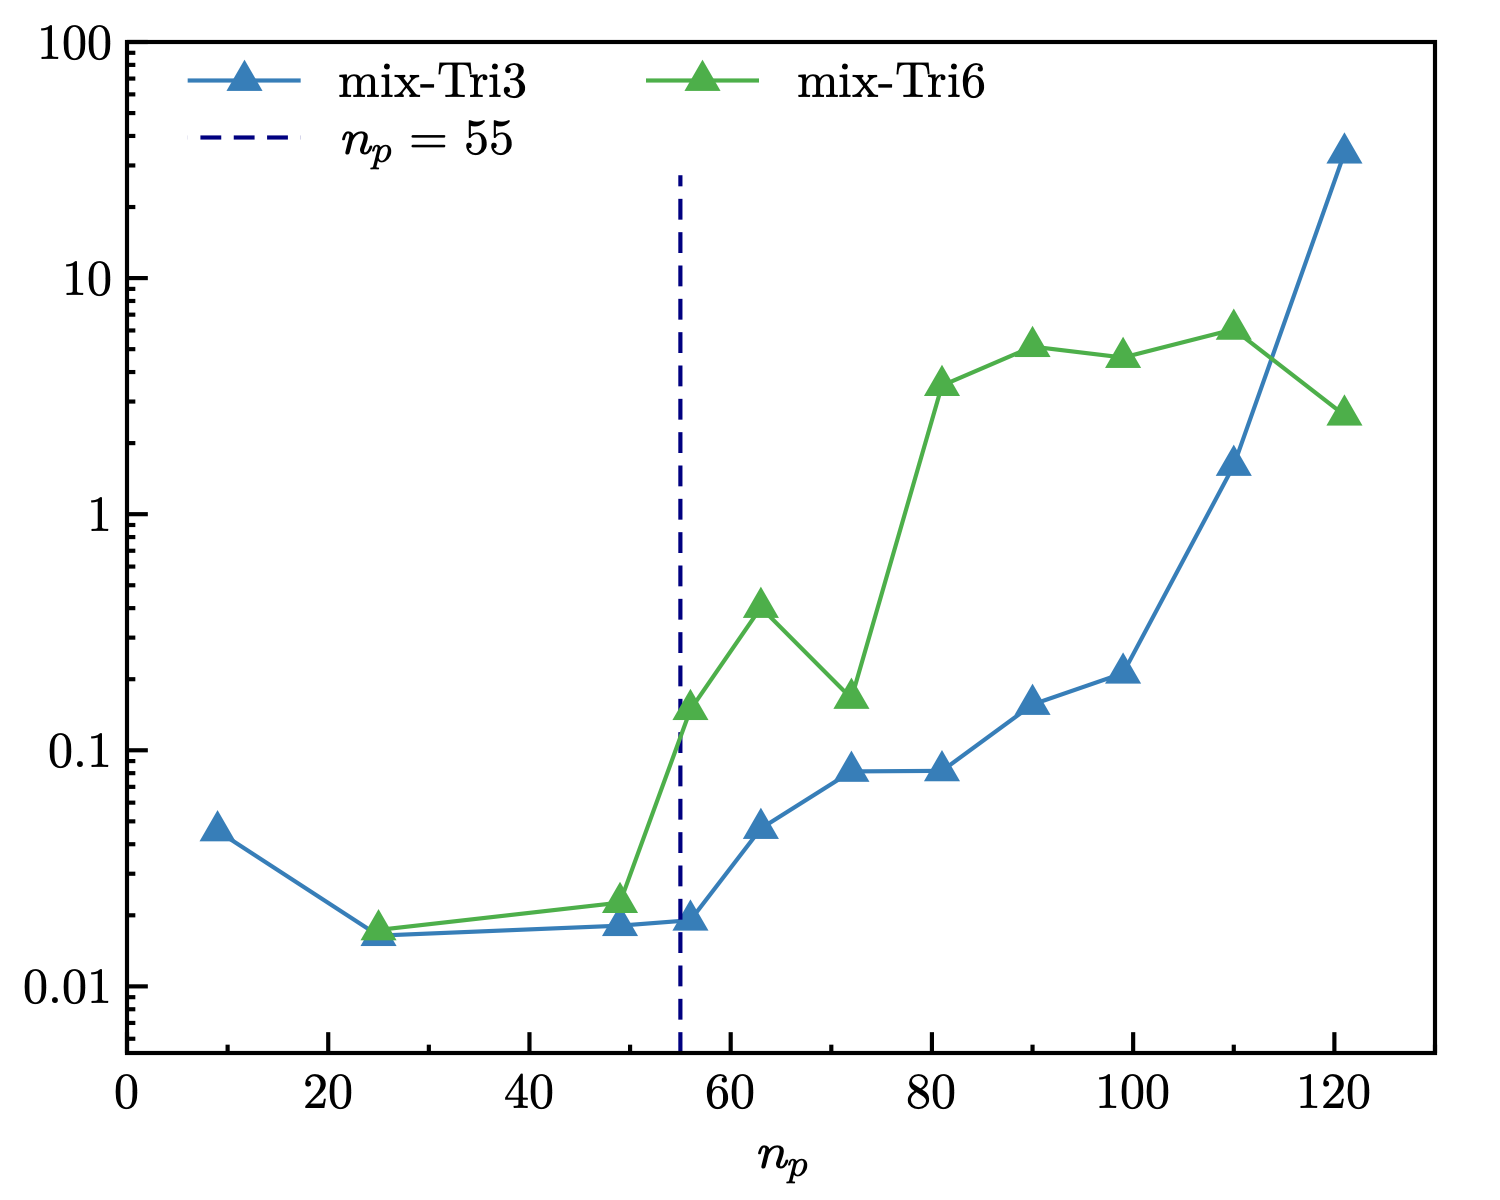
\includegraphics[width=0.45\textwidth]{figures/ch_4/plate_L2_p_4.png}}
        & \rotatebox{-90}{81 nodes} \\
          \raisebox{-0.7\height}{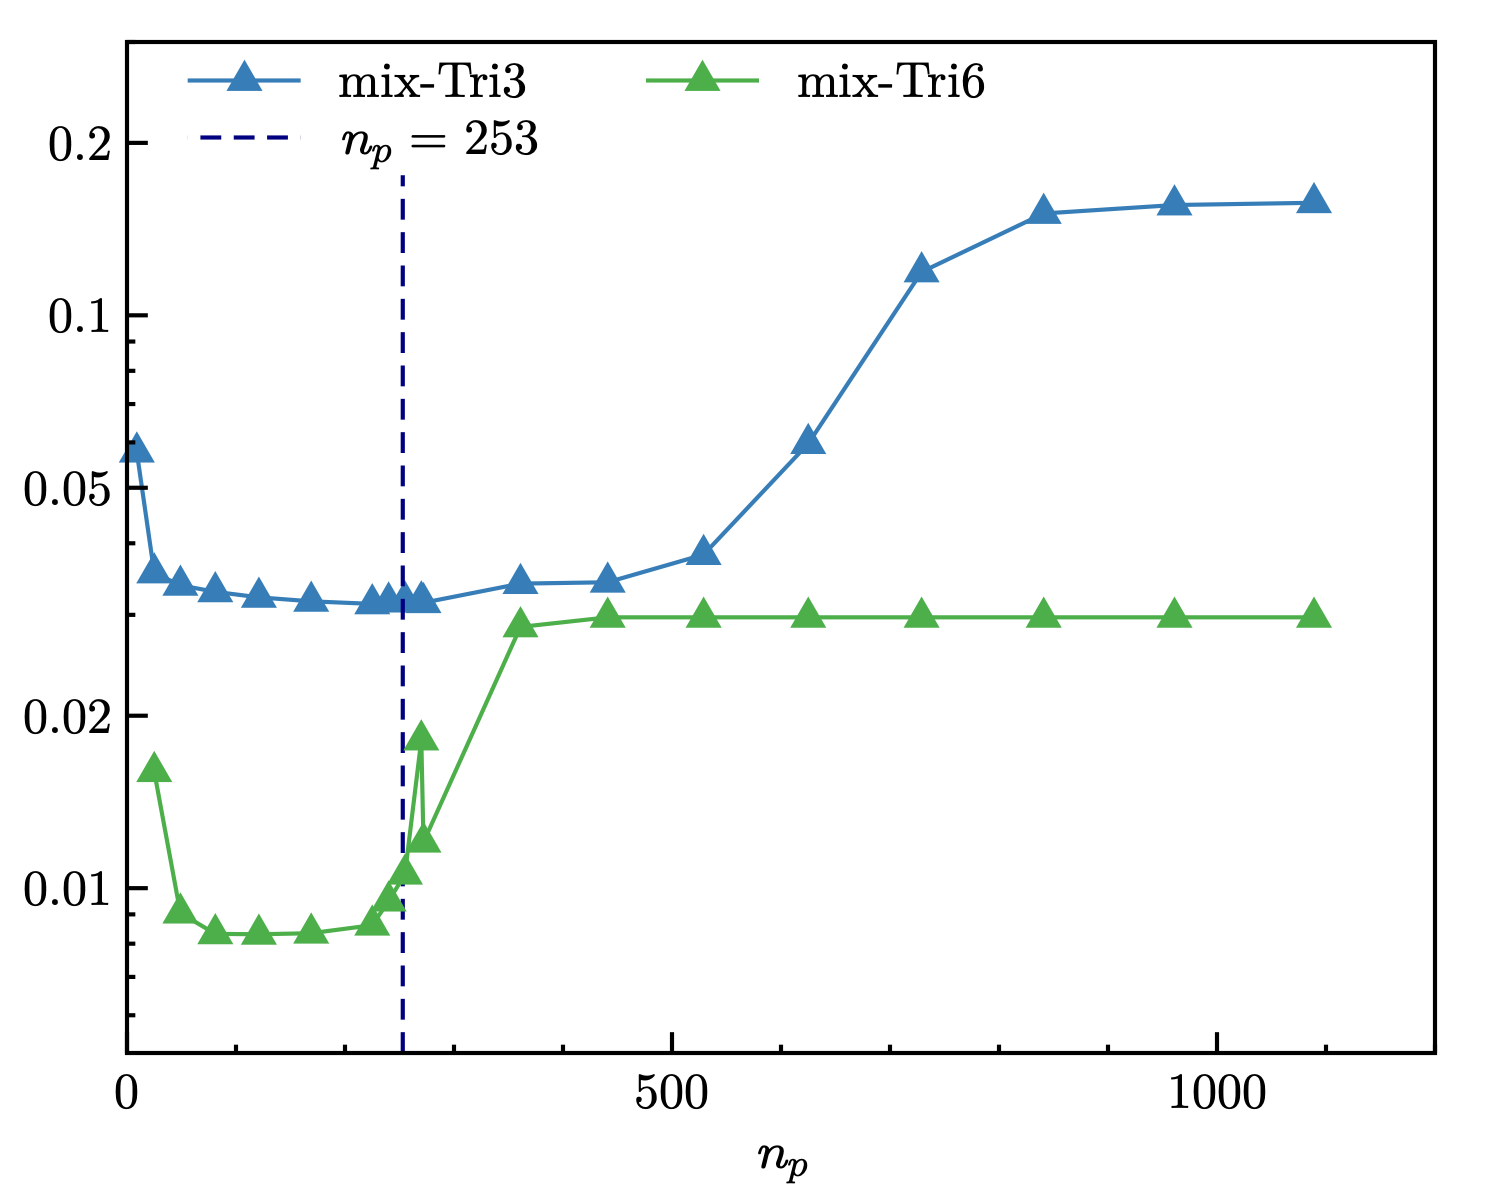
\includegraphics[width=0.45\textwidth]{figures/ch_4/plate_Hdev_8.png}}
        & \raisebox{-0.7\height}{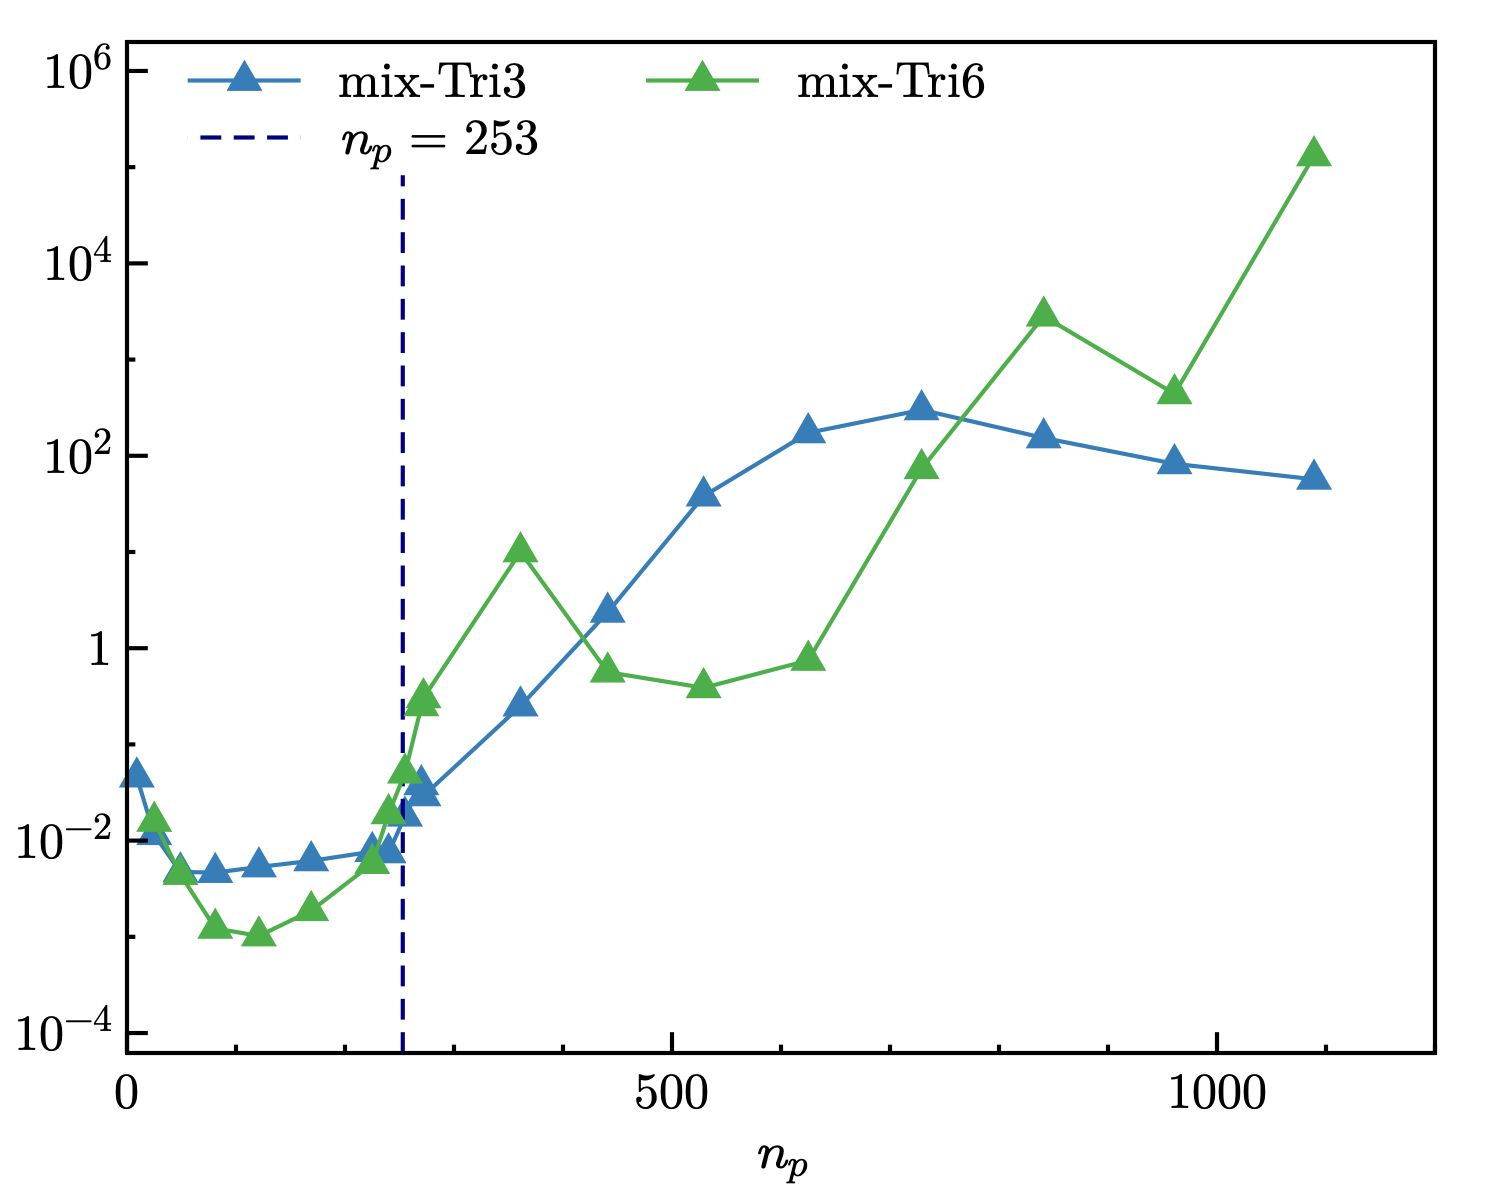
\includegraphics[width=0.45\textwidth]{figures/ch_4/plate_L2_p_8.png}}
        & \rotatebox{-90}{289 nodes} \\
          \raisebox{-0.7\height}{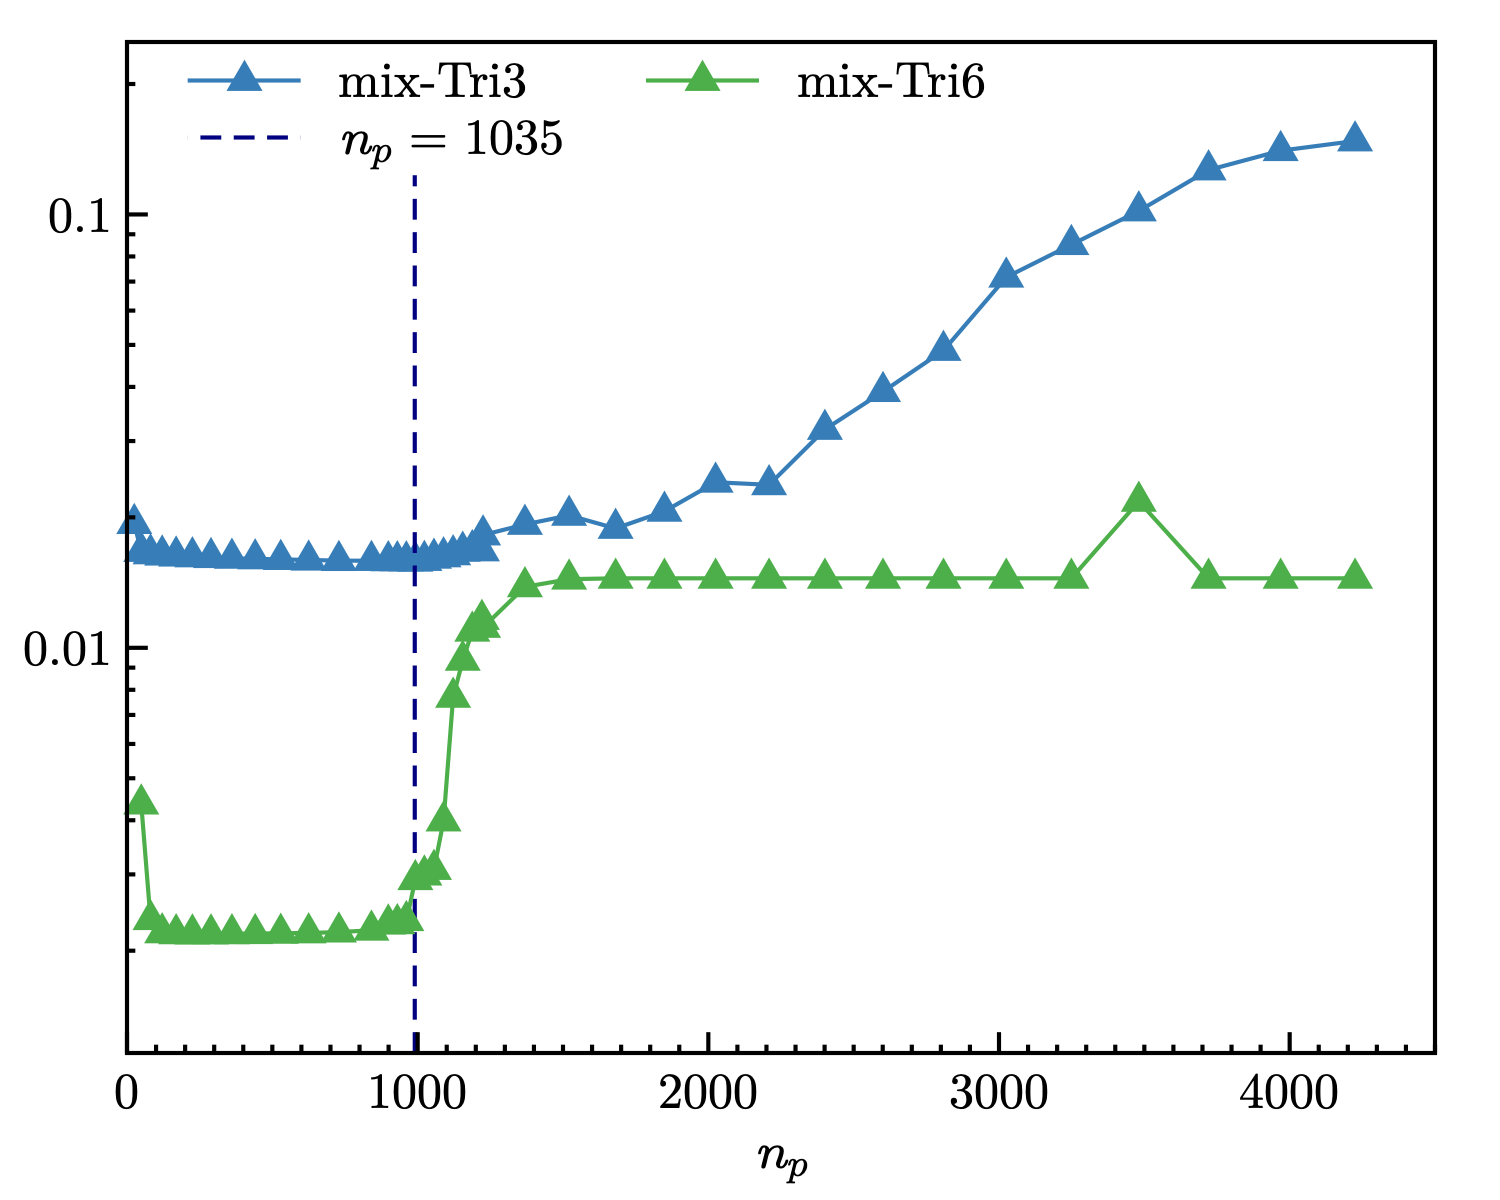
\includegraphics[width=0.45\textwidth]{figures/ch_4/plate_Hdev_16.png}}
        & \raisebox{-0.7\height}{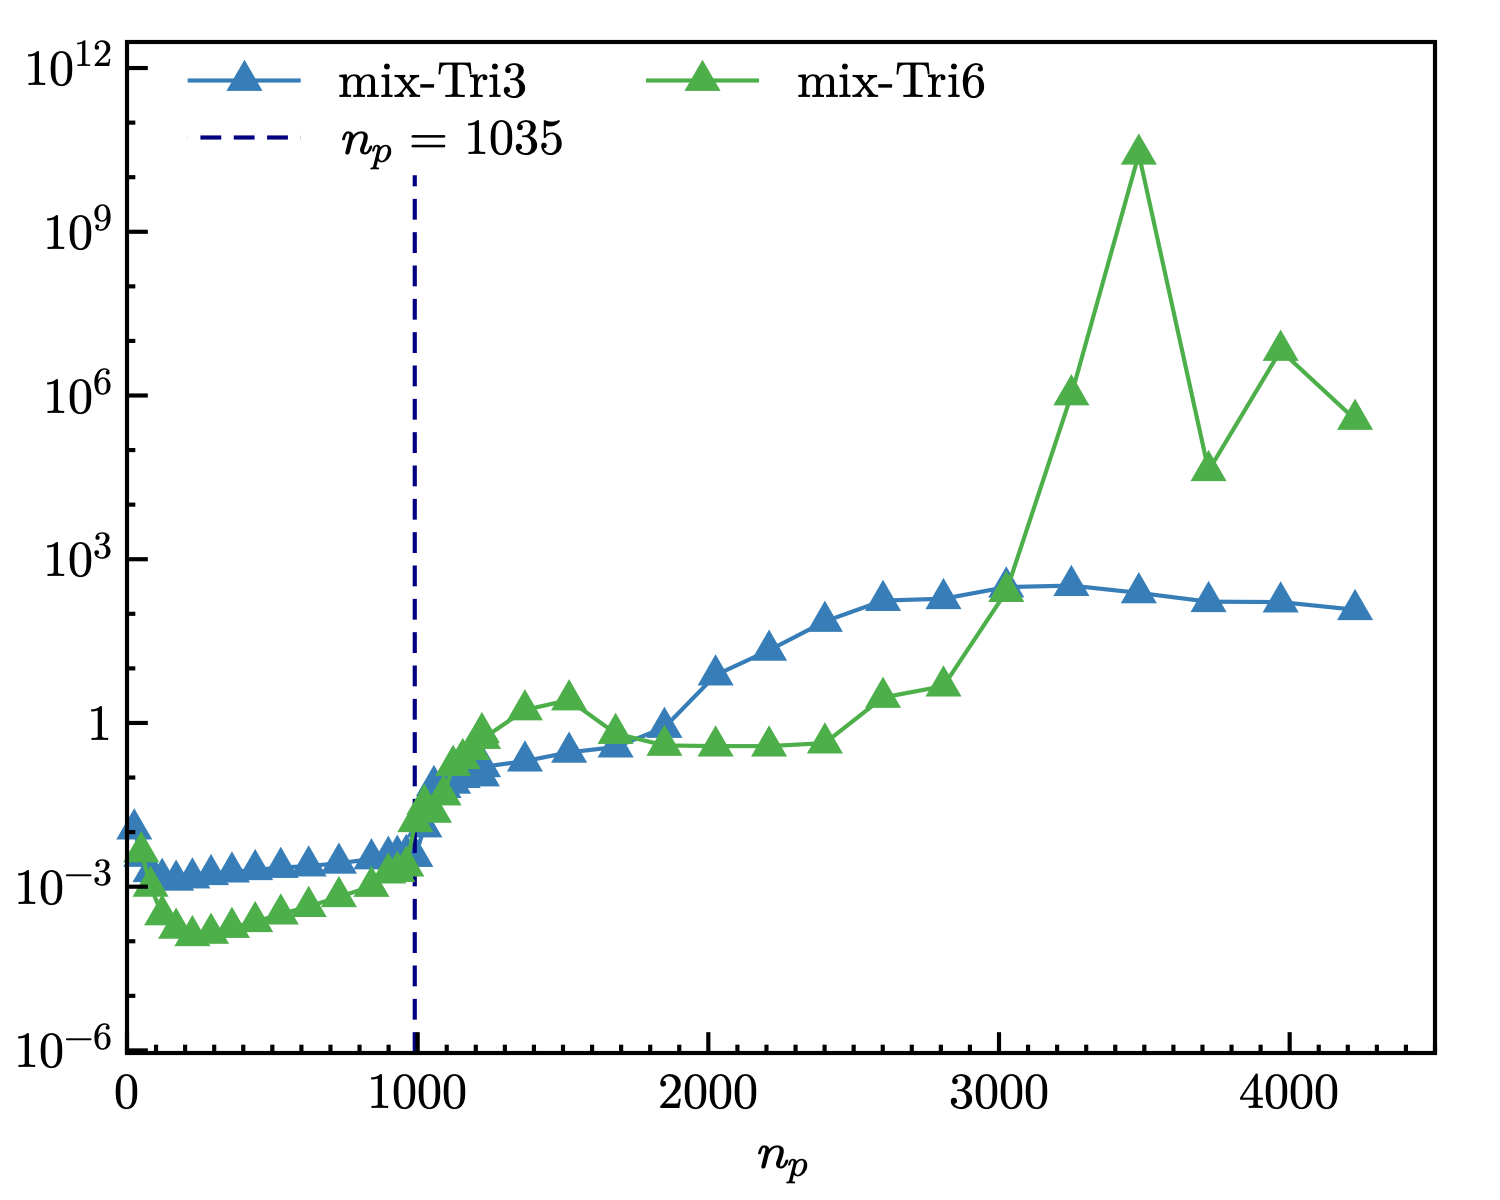
\includegraphics[width=0.45\textwidth]{figures/ch_4/plate_L2_p_16.png}}
        & \rotatebox{-90}{1089 nodes} \\
          \raisebox{-0.7\height}{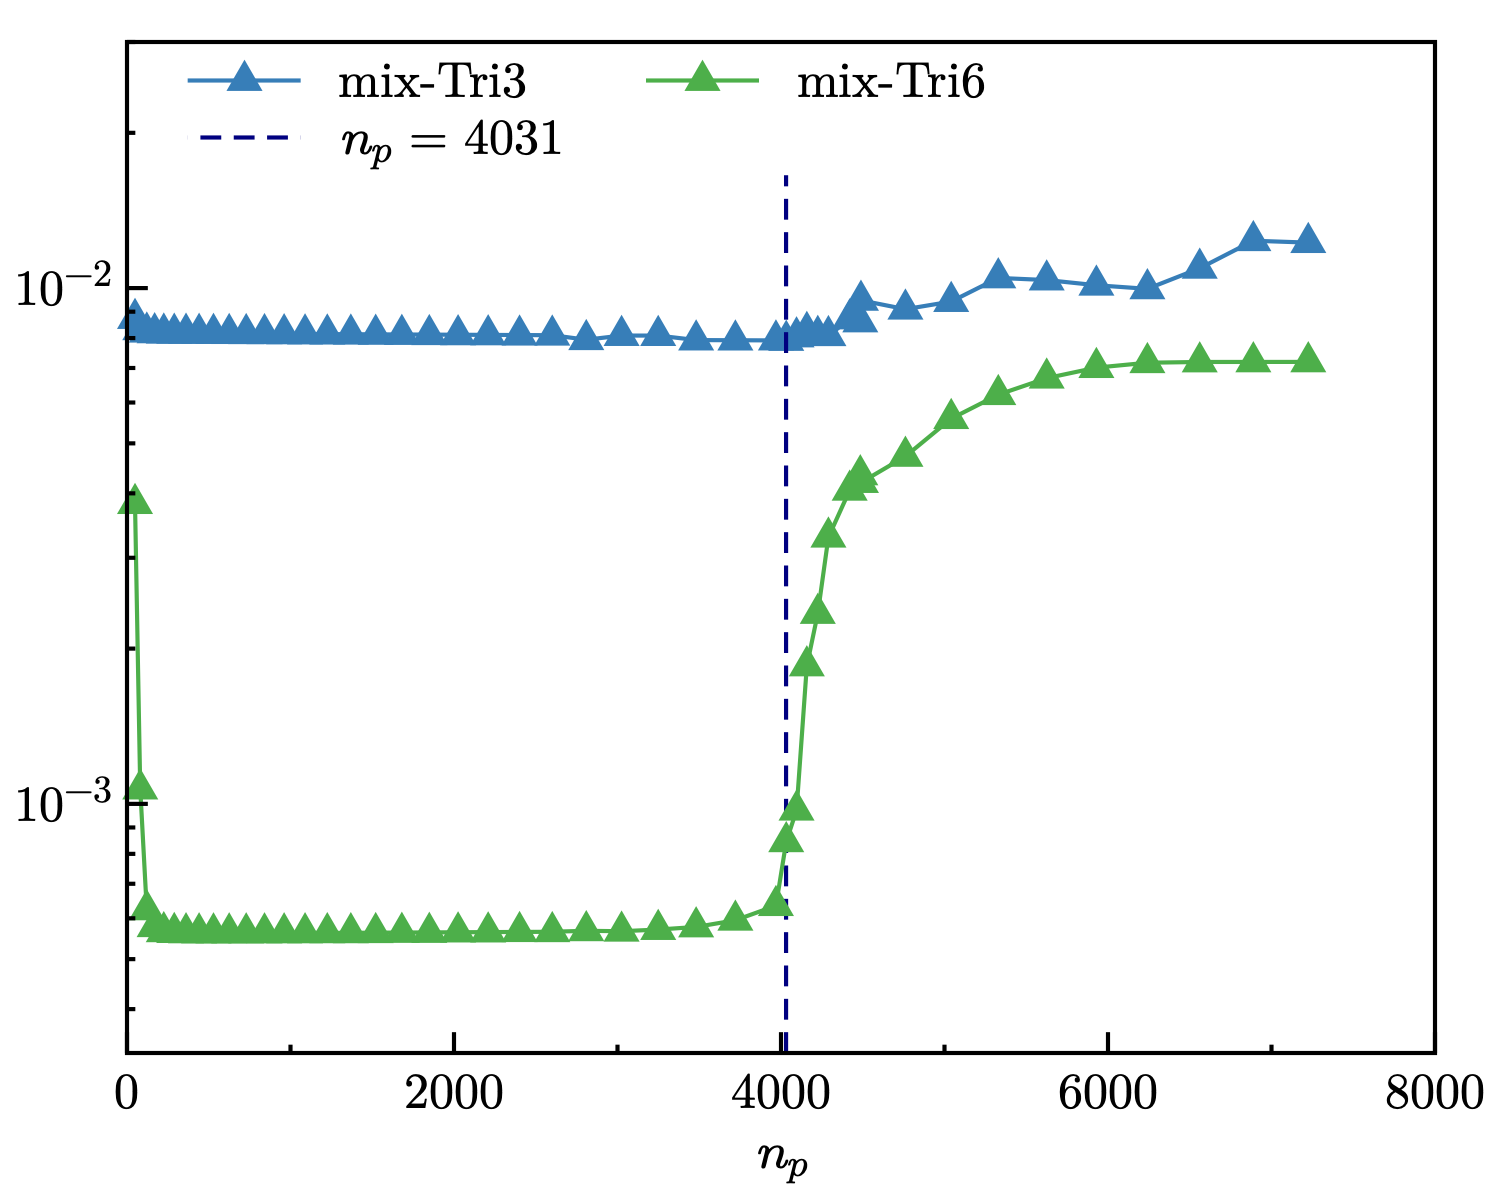
\includegraphics[width=0.45\textwidth]{figures/ch_4/plate_Hdev_32.png}}
        & \raisebox{-0.7\height}{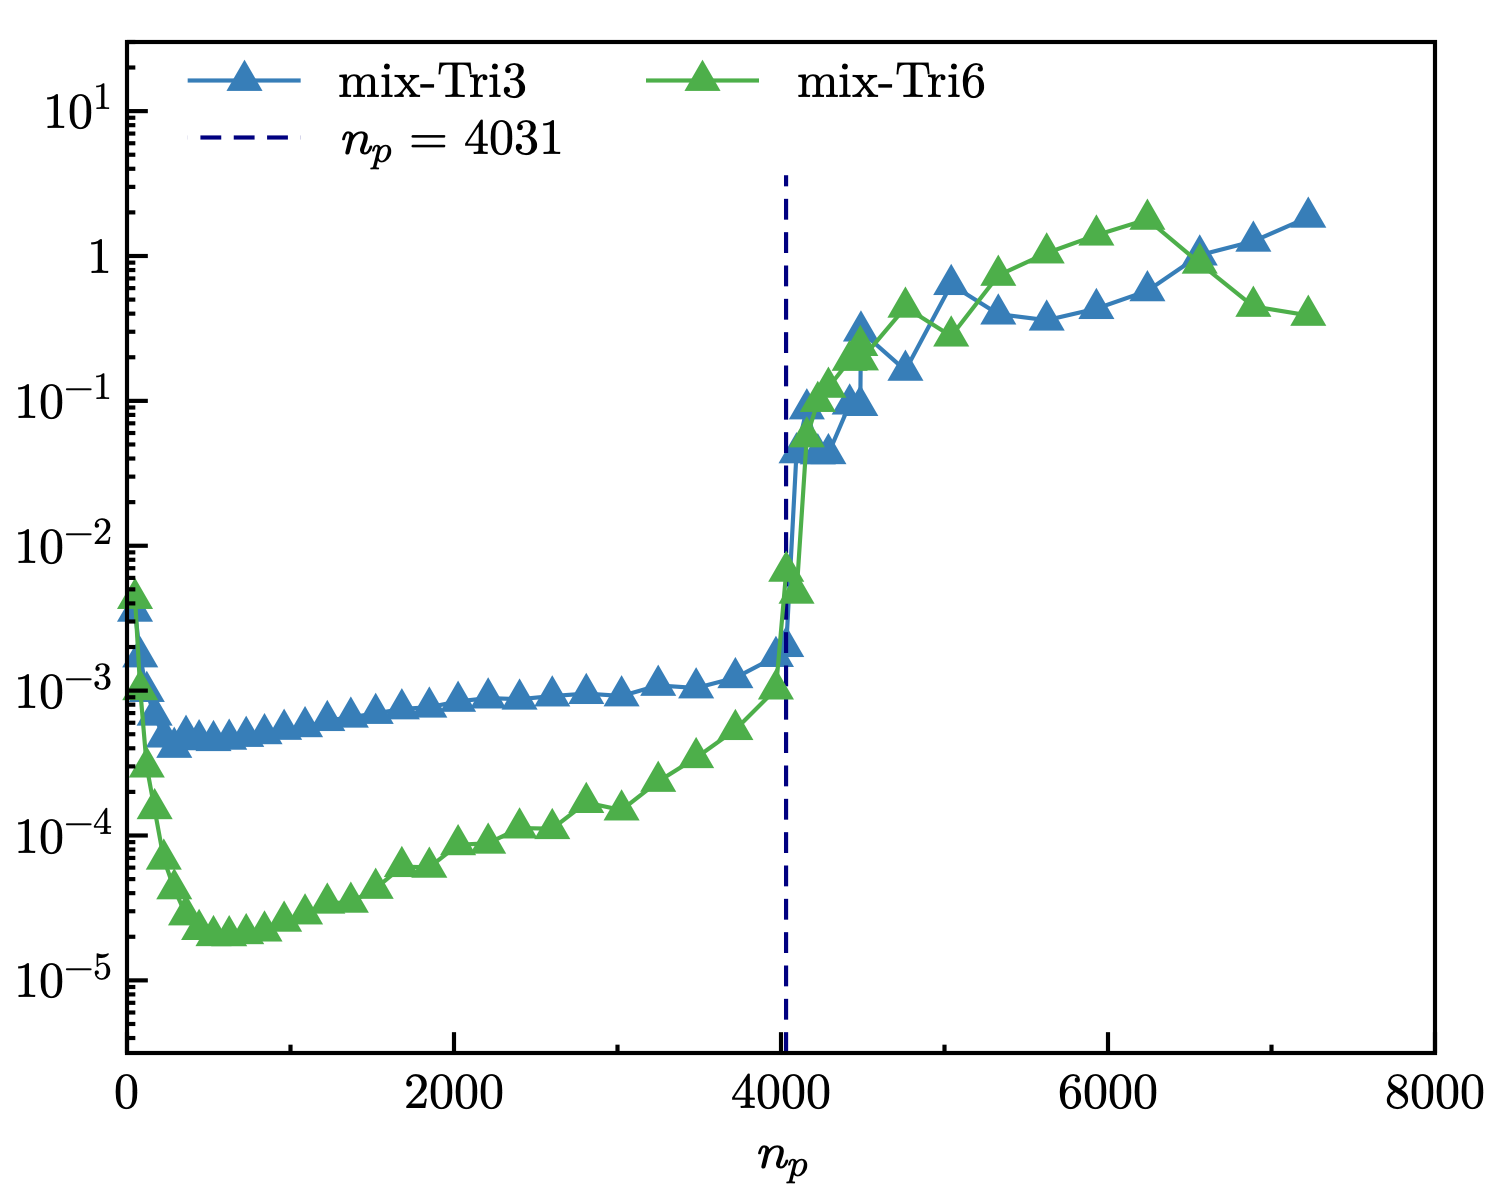
\includegraphics[width=0.45\textwidth]{figures/ch_4/plate_L2_p_32.png}}
        & \rotatebox{-90}{4225 nodes} \\
        \end{tabular}
    \end{subcaptiongroup}
    \caption{带孔方板问题误差与压力节点数的关系}\label{ch_4:fig:plate_with_hole_2}
\end{figure}

同样,选取Tri3和Tri6两种离散单元,分别对位移节点数$n_u=$81、289、1089、4225进行分析。图\ref{ch_4:fig:plate_with_hole_2}为相应的分析结果,其中虚线为本文提出的最优约束比下的压力节点数量。从图中可以看出:对于线性单元Tri3,当压力节点数$n_p$在一定值位移误差就趋于一定的精度,最优处处于稳定趋于之中。而对于二次单元Tri6,当$n_p$小于最优值时,位移误差达保持在较低水平。类似的趋势也体现在压力误差分析中,并且随着网格密度的增加,这一趋势更加明显。这些结果再次验证了当压力节点数$n_p$小于最优值时,离散方案能够获得高精度的数值解。

图\ref{ch_4:fig:plate_l2}为无限大平板问题Tri3和Tri6单元的位移误差和压力误差对比结果。从图中可以看出:在位移误差方面,Tri3单元的两种离散方案均能达到理论误差收敛率,而Tri6单元的传统混合离散方案则无法达到理论误差收敛率,本文所提方案则能达到理论误差收敛率。在压力误差方面,Tri3单元和Tri6单元的传统混合离散方案均无法达到理论误差收敛率,而所提方案则能够达到。这一结果进一步验证了本文所提离散方案在数值精度和稳定性方面的优越性。
\begin{figure}[H]
    \centering
    \begin{subcaptiongroup}
        \begin{tabular}{c@{\hspace{0pt}}c}
          \raisebox{-0.8\height}{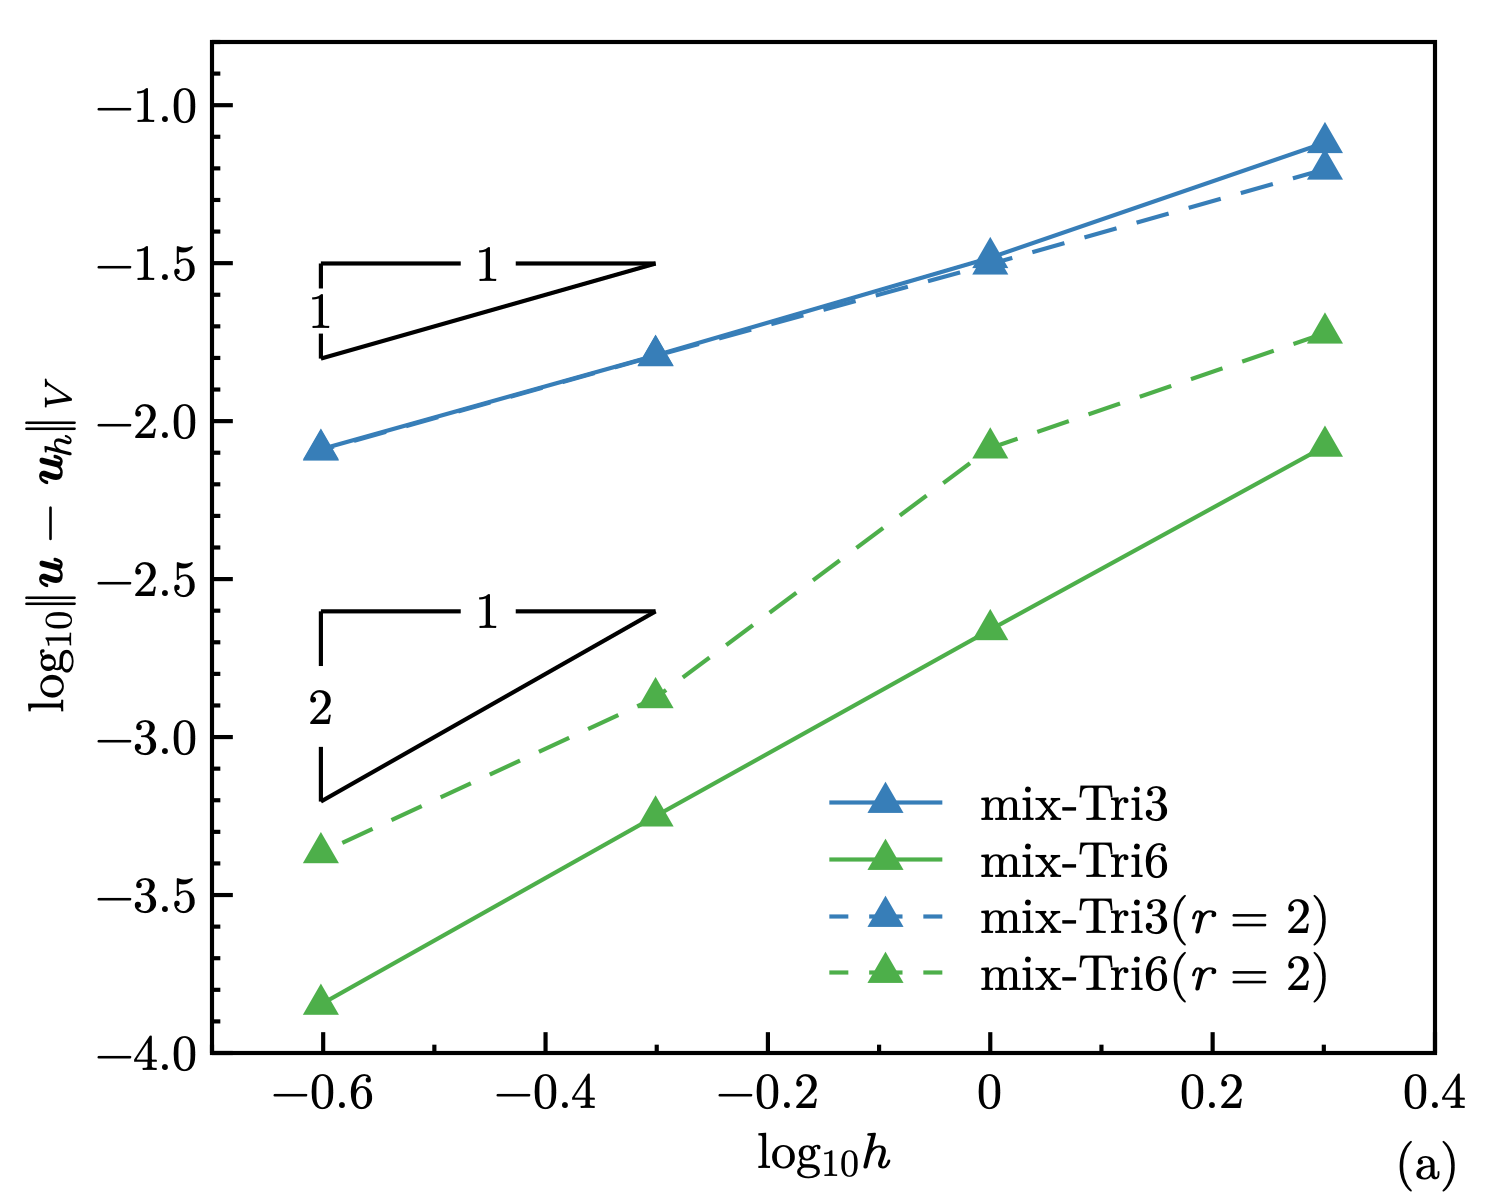
\includegraphics[width=0.5\textwidth]{figures/ch_4/plate_with_hole_Hdev.png}}
        & \raisebox{-0.8\height}{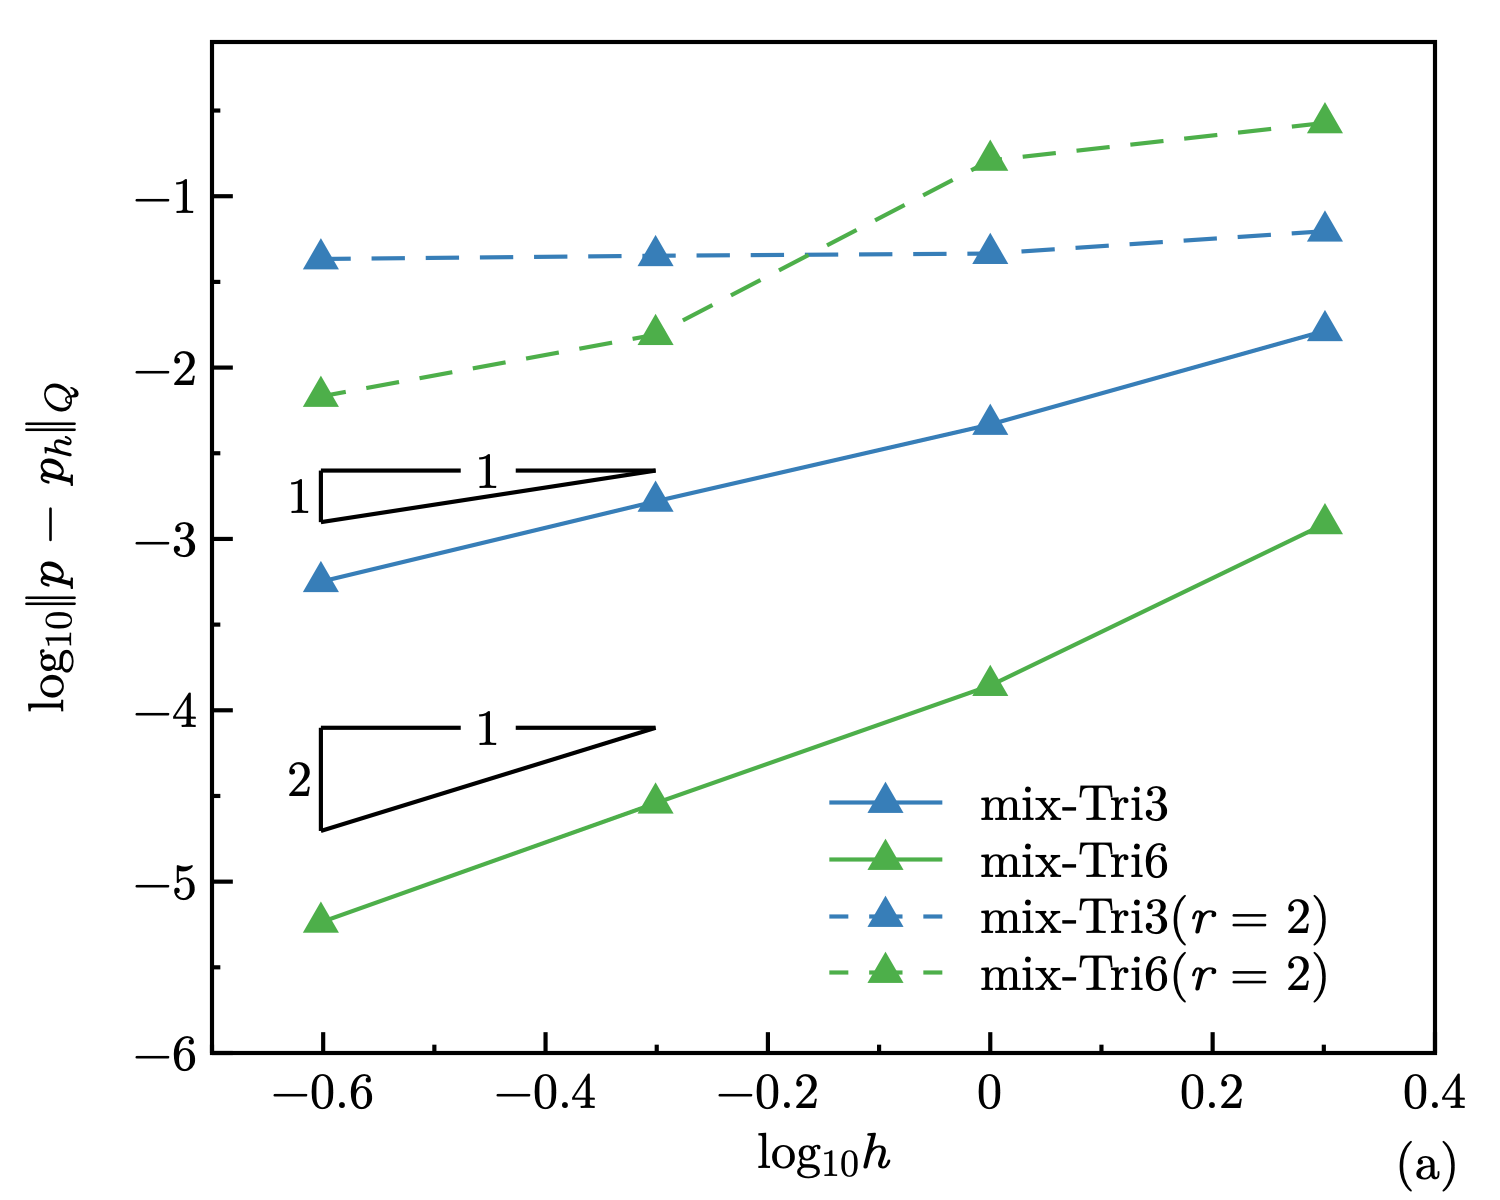
\includegraphics[width=0.5\textwidth]{figures/ch_4/plate_with_hole_L2_p.png}}\\
        \end{tabular}
    \end{subcaptiongroup}
    \caption{无限大平板问题误差对比}\label{ch_4:fig:plate_l2}
\end{figure}

\subsection{Cook membrane 问题}
考虑经典的Cook membrane 问题,膜的尺寸如图\ref{ch_4:fig:cook}所示,右端沿着$y$轴正方向施加外部荷载$P=6.25$,膜的材料系数为杨氏模量$E=70$、泊松比$\nu=0.5-10^{-8}$。在这种情况下,$A$点的位移参考解为:$u_A=28$。
\begin{figure}[!h]
    \centering 
        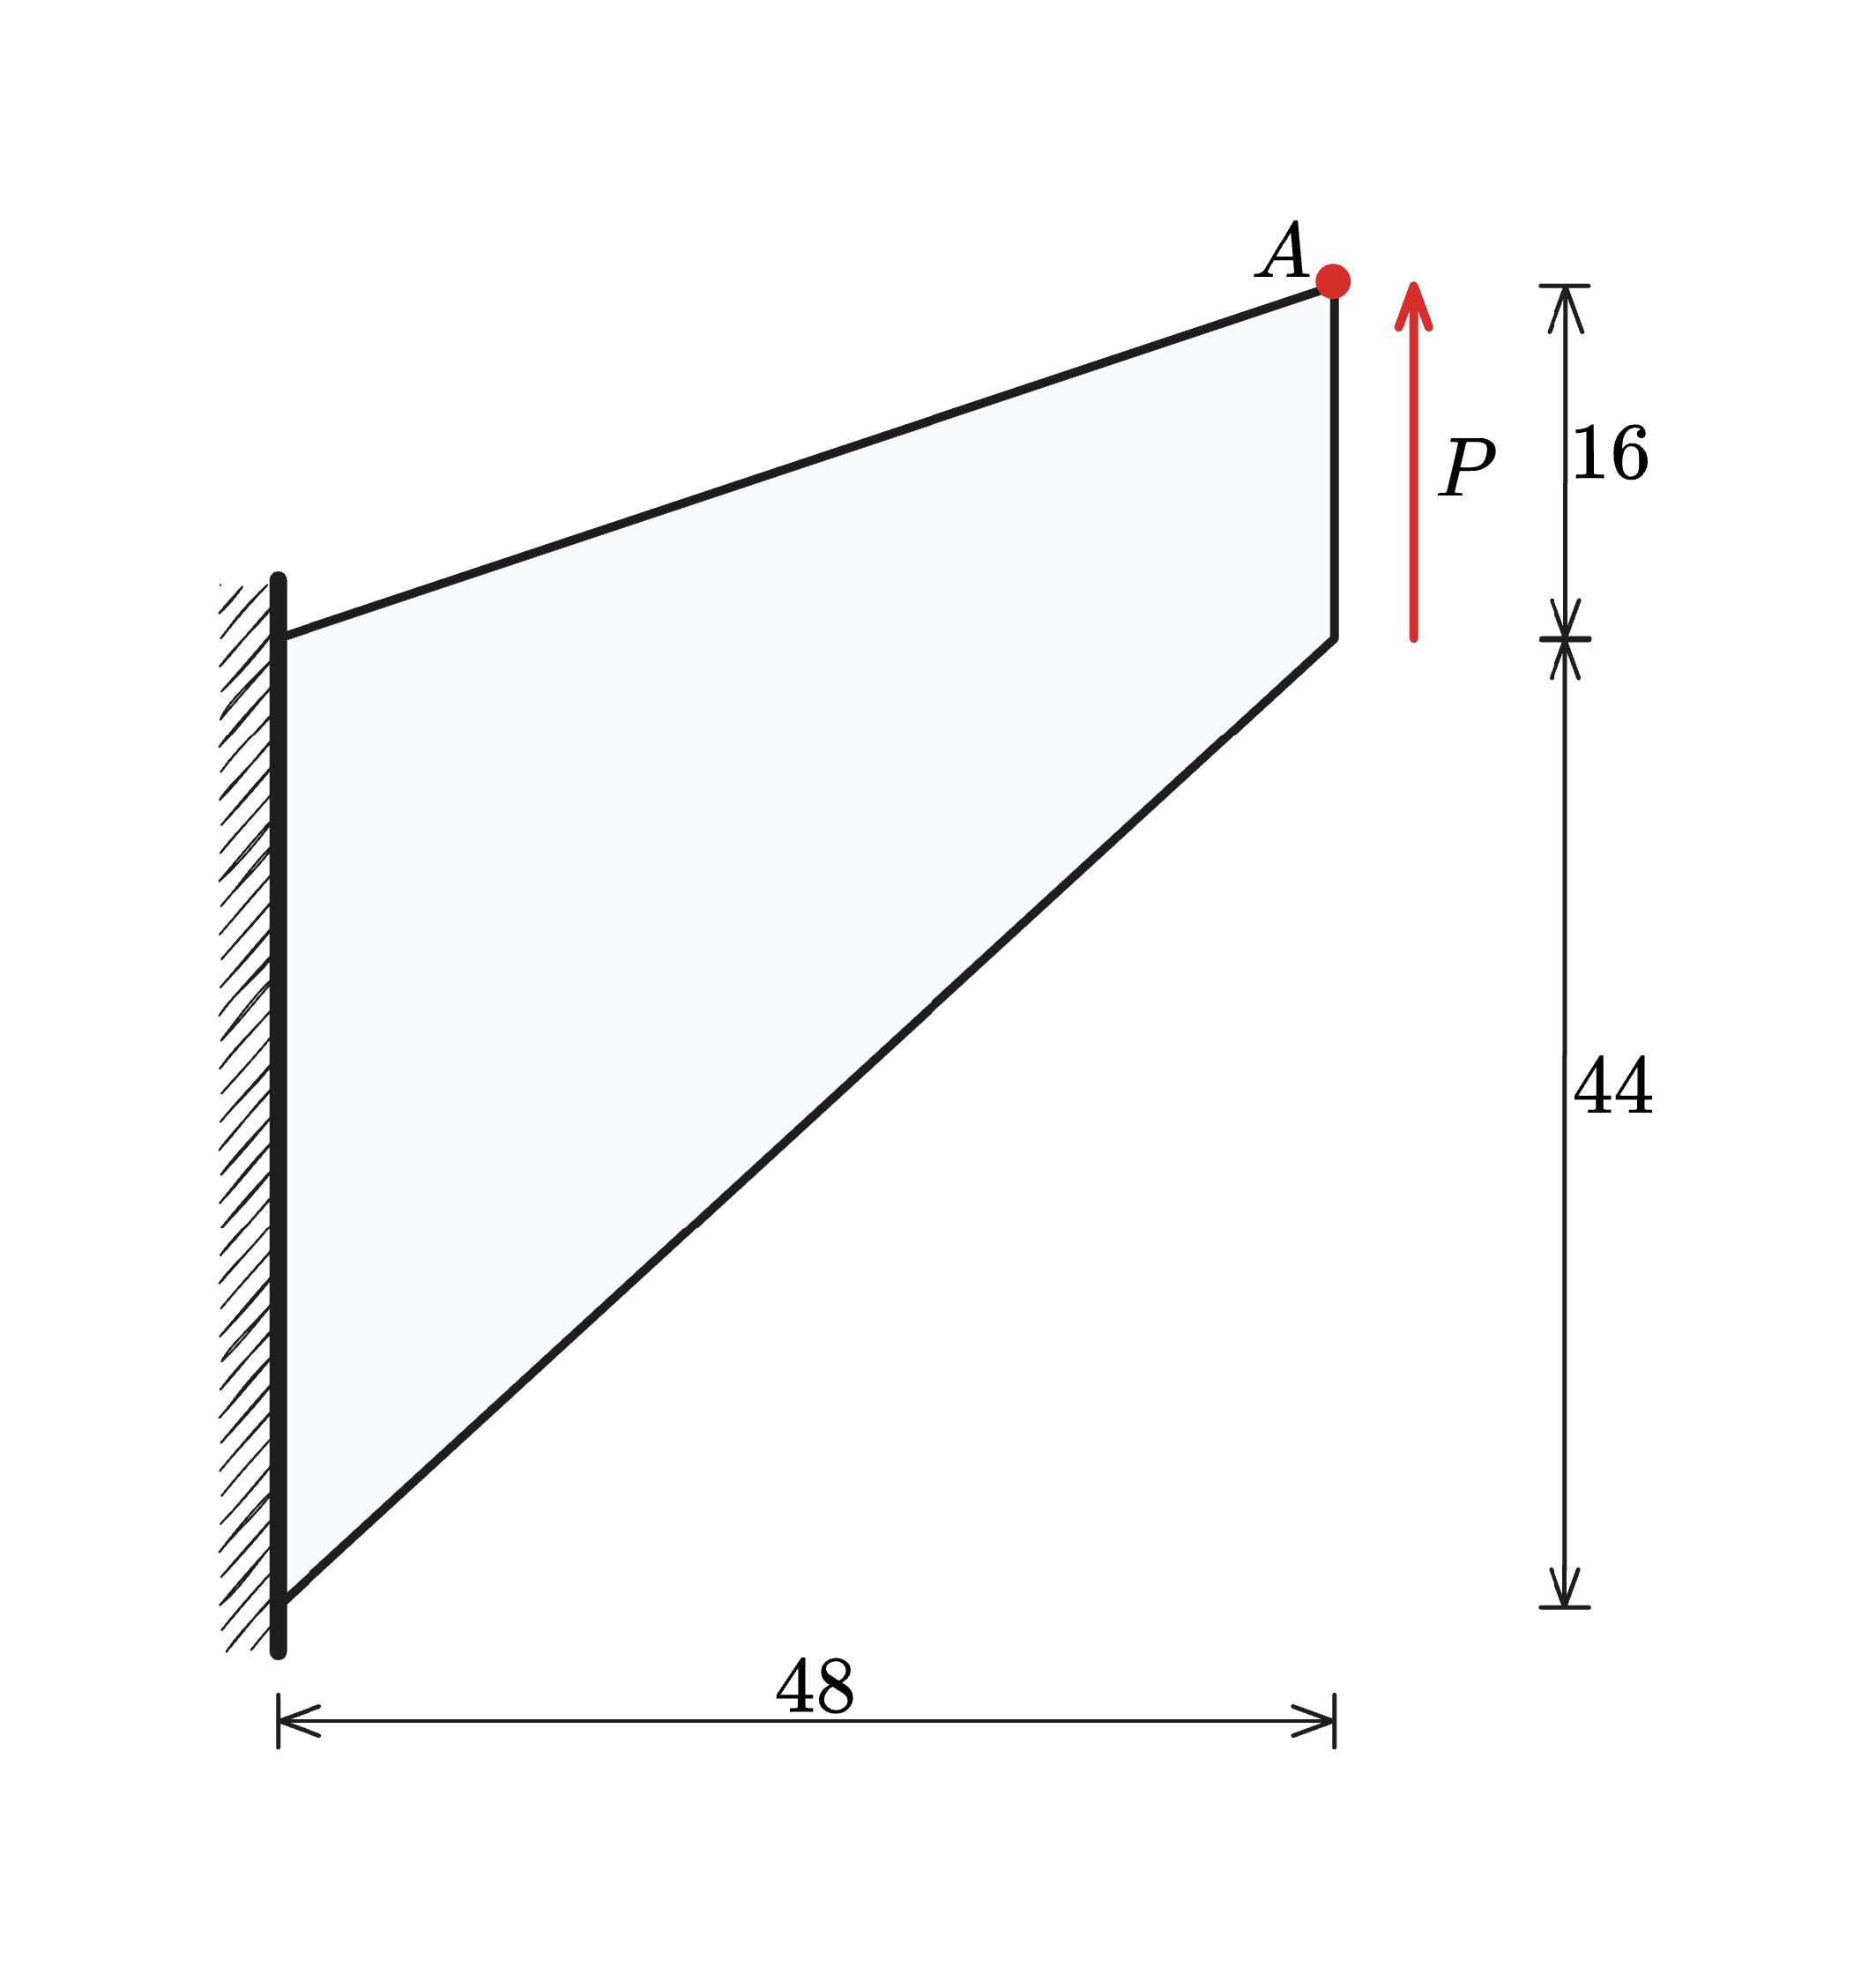
\includegraphics[scale=0.3]{figures/ch_4/cook.png}
        \caption{Cook membrane 问题模型}\label{ch_4:fig:cook}
\end{figure}

图\ref{ch_4:fig:Cook_membrane_p}和图\ref{ch_4:fig:Cook_membrane_p2}展示了Cook membrane 问题应力云图。通过对比四种不同离散单元的传统混合离散方案和本文所提混合离散方案,可以明显观察到:传统混合离散方案的压力云图出现了明显的振荡现象,而本文所提的混合离散方案则完全消除了这一振荡现象。这一对比结果充分证实了本文所提离散方案的数值稳定性,能够有效的避免压力振荡,从而获得更高精度的压力解。
\begin{figure}[!h]
    \centering
    \begin{subcaptiongroup}
        \begin{tabular}{c@{\hspace{0pt}}c@{\hspace{0pt}}c}
         $n_u$&传统混合离散方案&所提混合离散方案 \\
         \rotatebox{-90}{2145 nodes}& \raisebox{-0.7\height}{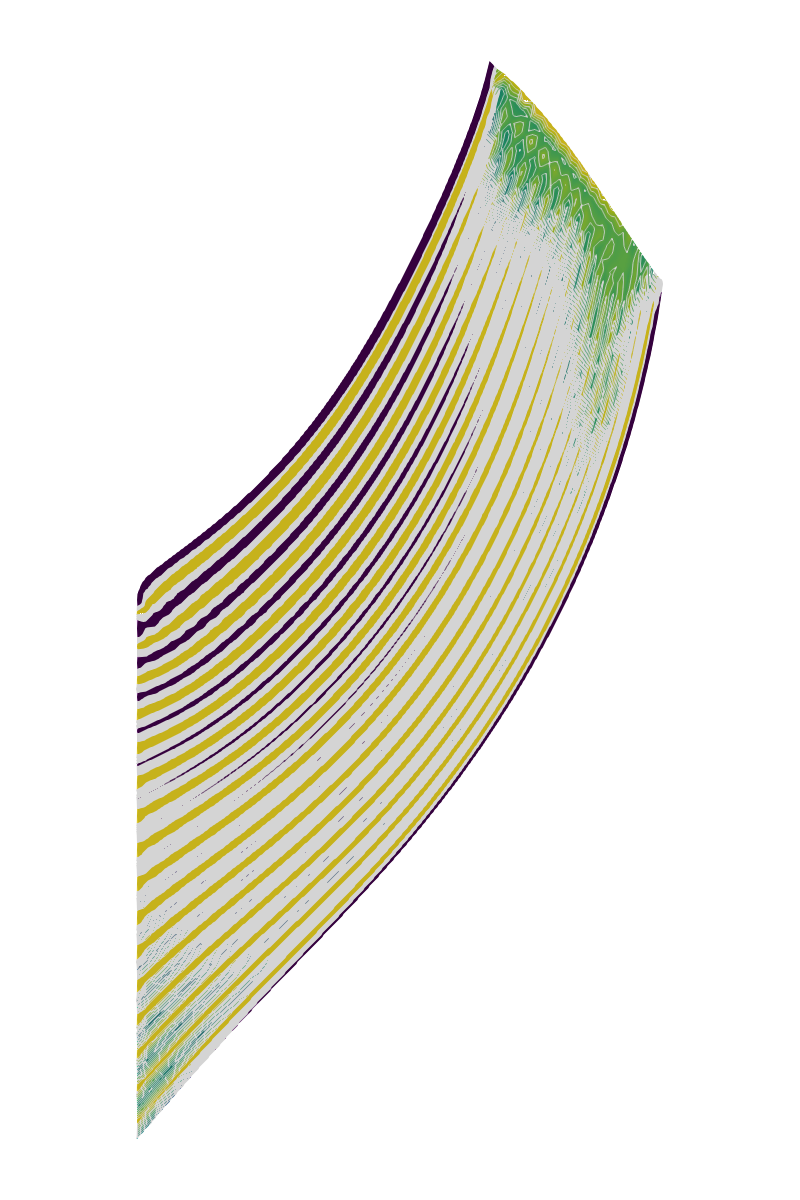
\includegraphics[width=0.45\textwidth]{figures/ch_4/cook_tri3_32_2145.png}}
        & \raisebox{-0.7\height}{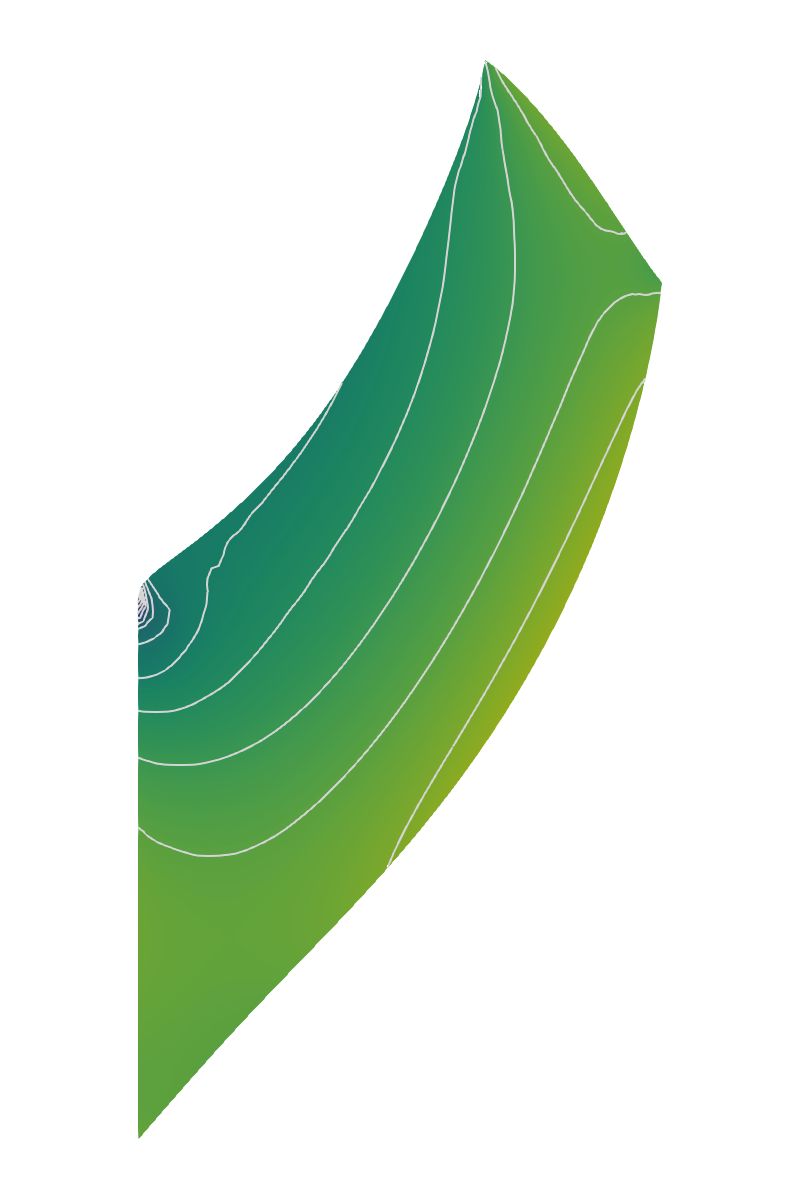
\includegraphics[width=0.45\textwidth]{figures/ch_4/cook_tri3_32_561.png}}\\
        Tri3&$n_p=2145$&$n_p=561$  \\
        \rotatebox{-90}{2145 nodes} &\raisebox{-0.7\height}{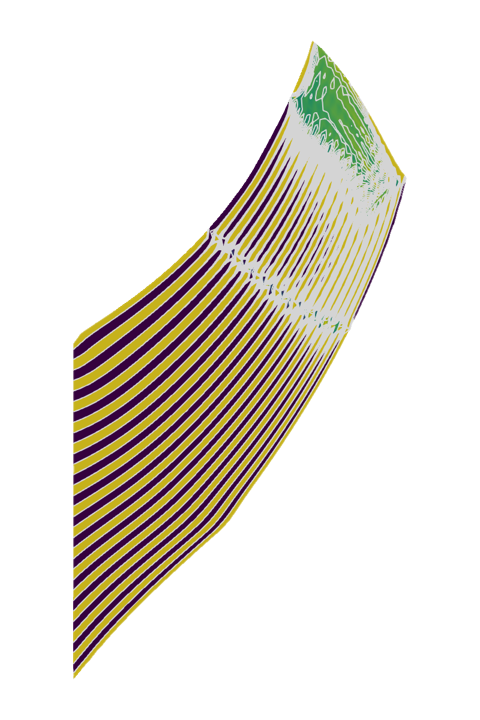
\includegraphics[width=0.45\textwidth]{figures/ch_4/cook_quad_32_2145.png}}
        & \raisebox{-0.7\height}{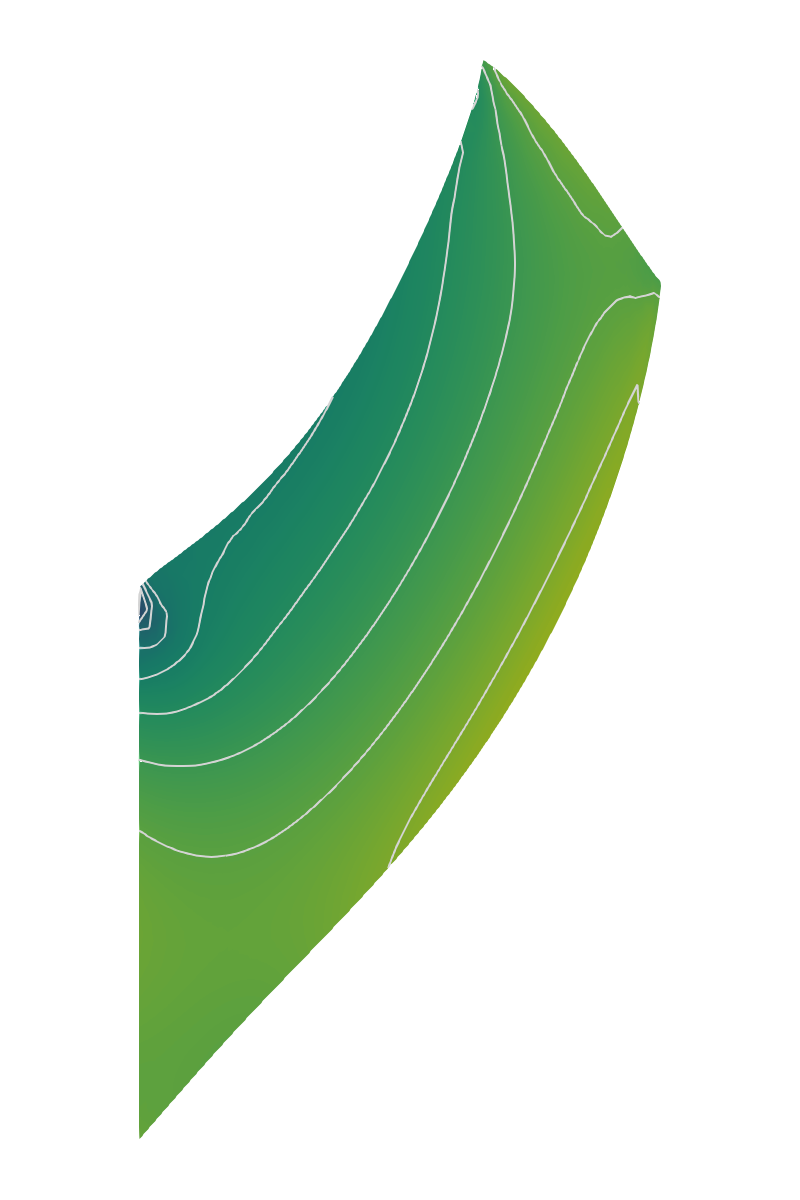
\includegraphics[width=0.45\textwidth]{figures/ch_4/cook_quad_32_561.png}}\\
        Quad4&$n_p=2145$&$n_p=561$ \\
        \end{tabular}
    \end{subcaptiongroup}
    \caption{Cook membrane 问题线性单元压力云图}\label{ch_4:fig:Cook_membrane_p}
\end{figure}

\begin{figure}[!h]
    \centering
    \begin{subcaptiongroup}
        \begin{tabular}{c@{\hspace{0pt}}c@{\hspace{0pt}}c}
        $n_u$&传统混合离散方案&所提混合离散方案 \\
        \rotatebox{-90}{8385 nodes}& \raisebox{-0.7\height}{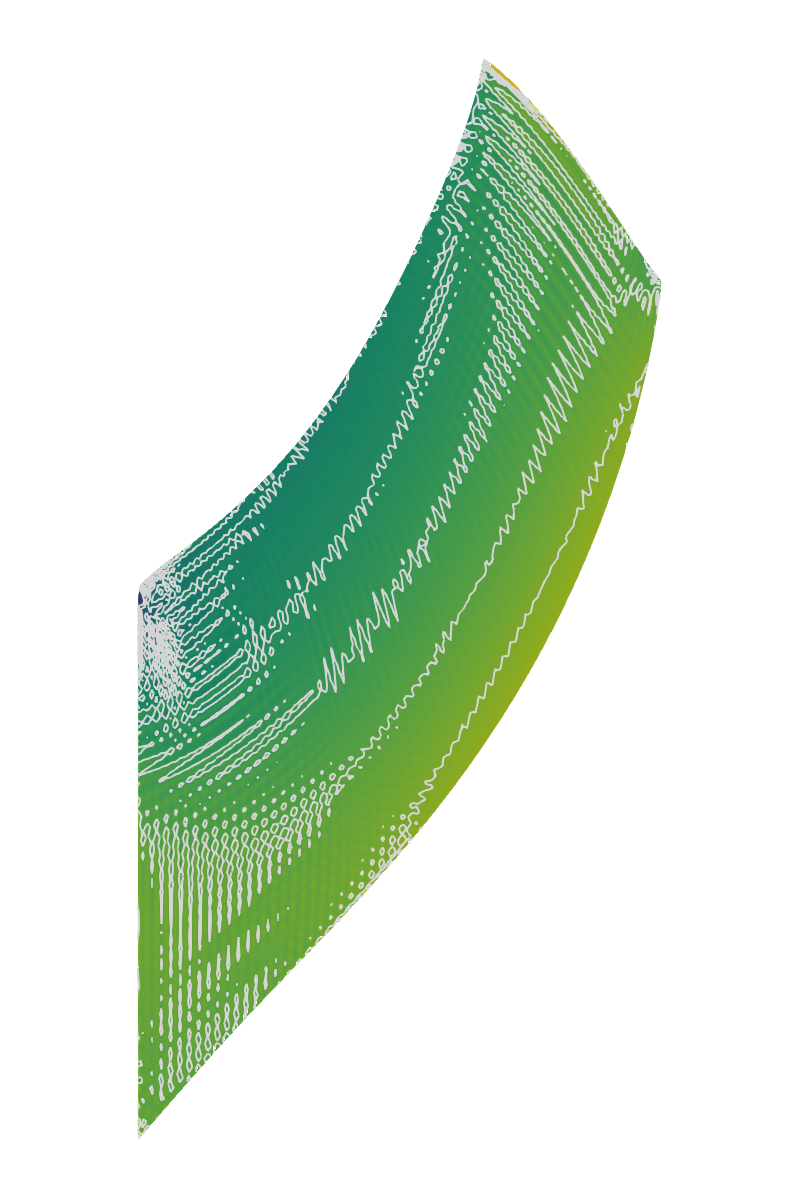
\includegraphics[width=0.45\textwidth]{figures/ch_4/cook_tri6_32_8385.png}}
        & \raisebox{-0.7\height}{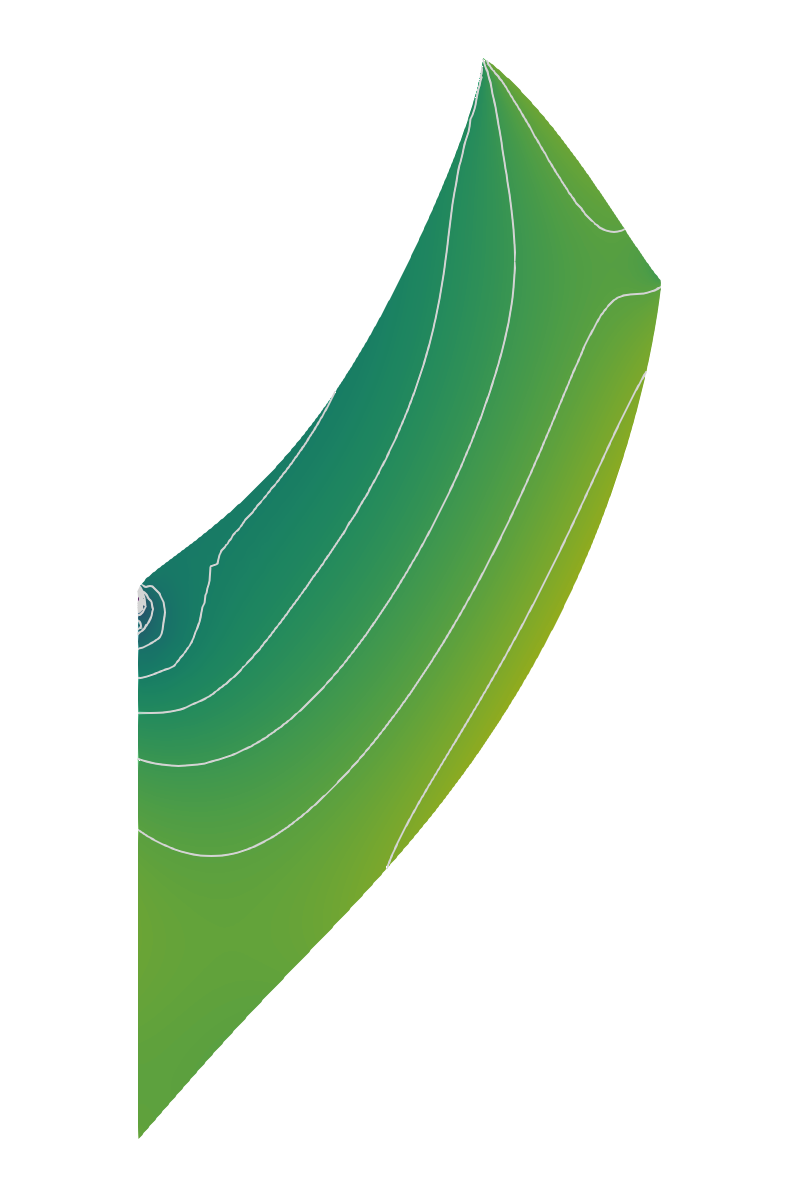
\includegraphics[width=0.45\textwidth]{figures/ch_4/cook_tri6_32_2145.png}} \\
        Tri6&$n_p=8385$&$n_p=2145$  \\
        \rotatebox{-90}{6337 nodes} & \raisebox{-0.7\height}{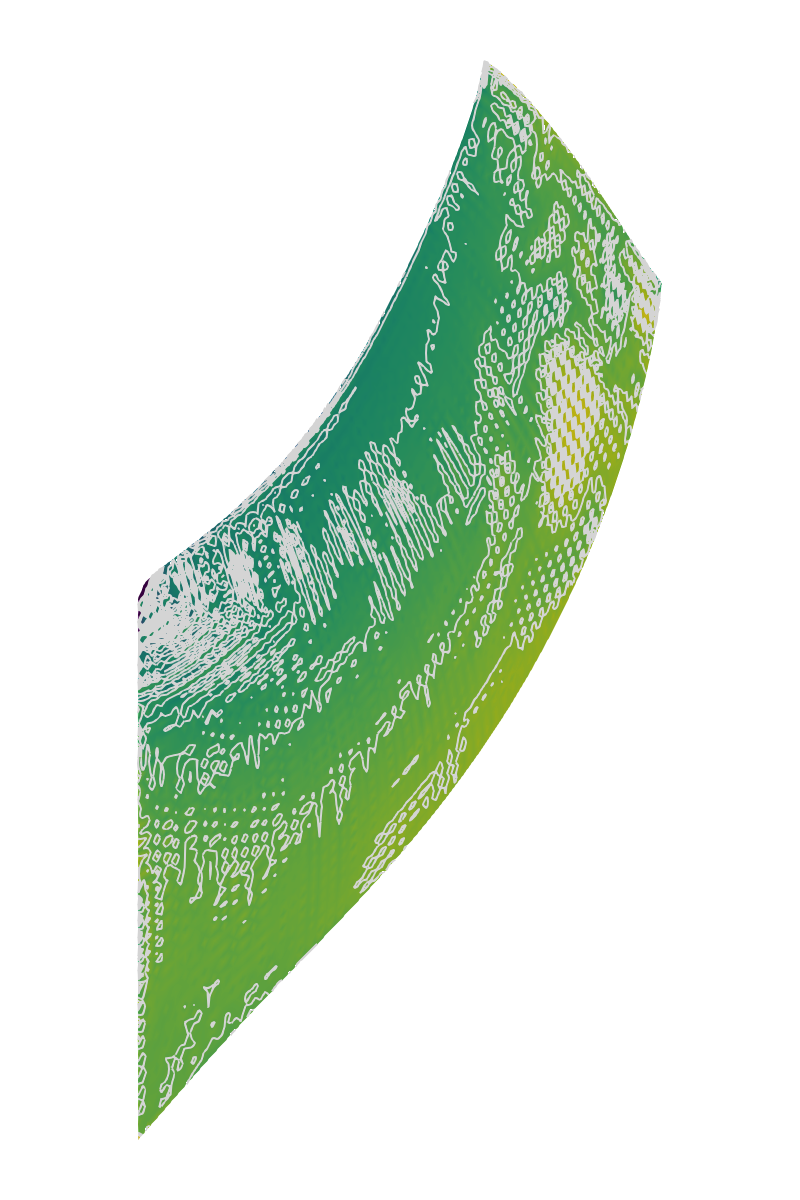
\includegraphics[width=0.45\textwidth]{figures/ch_4/cook_quad8_32_6337.png}}
        & \raisebox{-0.7\height}{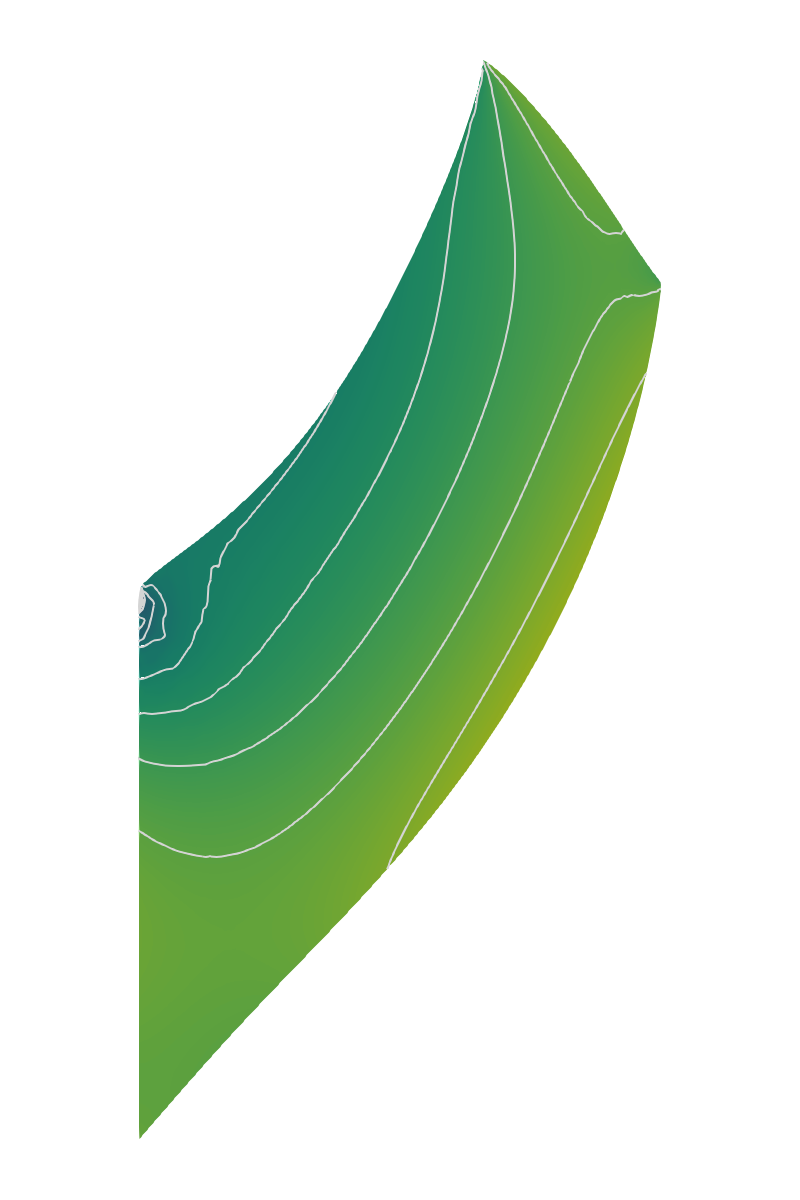
\includegraphics[width=0.45\textwidth]{figures/ch_4/cook_quad8_32_2145.png}} \\
        Tri8&$n_p=6337$&$n_p=2145$  \\
        \end{tabular}
    \end{subcaptiongroup}
    \caption{Cook membrane 问题二次单元压力云图}\label{ch_4:fig:Cook_membrane_p2}
\end{figure}
\section{小结}

本章提出了一种基于LBB稳定性条件的有限元无网格混合离散方案,用于求解体积不可压材料体积自锁问题。
首先,对再生核无网格近似理论进行了系统讨论,详细说明了无网格形函数的构造过程,将混合公式中的压力采用无网格形函数进行离散,可实现对压力节点数量的灵活调控,从而有效控制了体积约束比。
随后,基于考虑约束比的LBB稳定系数估计和最优约束比取值范围,对四种的离散单元的四个位移节点数的LBB稳定性系数进行了系统性测试,最终提出了一种同时满足LBB稳定性条件、兼具简易性与稳定性的有限元无网格混合离散方案。
最后,通过对典型体积不可压算例的系统验证,证实了所提最优体积约束比取值范围以及无网格有限元混合离散方案的正确性。数值结果表明,该混合离散方案不仅具有节点布置简便的优势,而且能够确保数值计算的稳定性,同时消除了压力振荡现象。
